\chapter{Безконтекстни езици и стекови автомати}


Ще започнем като разгледаме понятието извод в граматика в най-общия му вид.
Граматиките се разделят на няколко вида в зависимост от това какви {\em ограничения} налагаме върху правилата на граматиката. В следващите няколко глави ще разгледаме различни ограничения. 
След това ще разгледаме някои класове от граматики като ще се концентрираме основно върху безконтекстните граматики.

\thispagestyle{empty}
\begin{tikzpicture}
\pgftransformscale{.7}

\draw[very thick] (10,0) -- (-10,0);

% \draw (-3,0) parabola bend (0,3.5) (3,0);
% \node at (0,2.2) {
% 	\begin{tabular}{c}
%           Крайни \\ езици
% 	\end{tabular}
% };

\draw (-5.5,0) parabola bend (0,6) (5.5,0);
\node at (0,4.8) {
  \begin{tabular}{c}
    Регулярни \\ граматики
  \end{tabular}
};

\draw (-7.5,0) parabola bend (0,8) (7.5,0);
\node at (0,6.8) {  
  \begin{tabular}{c}
    Безконтекстни \\ граматики
  \end{tabular}
};

\draw (-9.5,0) parabola bend (0,10) (9.5,0);
\node at (0,8.8) {  
  \begin{tabular}{c}
    Контекстни граматики
  \end{tabular}
};

\draw[very thick] (-9.5,0) parabola bend (0,12.5) (9.5,0);
\node at (0,11) {
  \begin{tabular}{c}
    Неограничени\\ граматики
  \end{tabular}
};
\end{tikzpicture}


\section{Неограничени граматики}
\index{граматика!неограничена}
\label{sect:regular-grammar}
\mynote{На англ. {\em unrestricted grammar}. Това е тип 0 граматики в йерархията на Чомски \cite[стр. 220]{hopcroft1}.}
{\bf Неограничена граматика} e наредена четворка от вида
\[G = (V, \Sigma, R, S),\]
където:
\begin{itemize}
\item
  $V$ е крайно множество от {\em променливи} (нетерминали);
\item
  $\Sigma$ е крайно множество от {\em букви} (терминали), $\Sigma \cap V = \emptyset$;
\item
  \mynote{В \cite{hopcroft1} правилата се наричат {\em productions} или {\em production rules}.}
  $R \subseteq (V\cup\Sigma)^+ \times (V \cup \Sigma)^\star$ е крайно множество от {\em правила}.
  За по-добра яснота, обикновено правилата $(\alpha, \beta) \in R$ ще означаваме като 
  $\alpha \to_G \beta$.
\item
  $S \in V$ е началната променлива (нетерминал). 
\end{itemize}

\index{граматика!извод}
Удобно е да дефинираме извод на думата $\beta$ от думата $\alpha$ в граматиката $G$ за $\ell$ стъпки, което ще означаваме като $\alpha \derive{\ell}_G \beta$,
с индукция по броя на стъпките $\ell$ по следния начин:
\mynote{Обърнете внимание, че имаме недетерминизъм в тази дефиниция на извод. Също така, понякога ,за удобство, ще пишем просто $\derive{\ell}$ вместо $\derive{\ell}_G$,
  когато се знае за коя граматика говорим.}
\begin{prooftree}
  \AxiomC{}
  \UnaryInfC{$\alpha \derive{0}_G \alpha$}
\end{prooftree}

\begin{prooftree}
  \AxiomC{$\alpha \to_G \gamma$}
  \AxiomC{$\gamma \derive{\ell}_G \beta$}
  \BinaryInfC{$\alpha \derive{\ell+1}_G \beta$}
\end{prooftree}

\begin{prooftree}
  \AxiomC{$\alpha_1 \derive{\ell_1}_G \beta_1$}
  \AxiomC{$\alpha_2 \derive{\ell_2}_G \beta_2$}
  \BinaryInfC{$\alpha_1\cdot\alpha_2 \derive{\ell_1+\ell_2}_G \beta_1\cdot \beta_2$}
\end{prooftree}

\mynote{В частност имаме следното:
\begin{prooftree}
  \AxiomC{$\alpha \to_G \beta$}
  \UnaryInfC{$\alpha \derive{1}_G \beta$}
\end{prooftree}
}

Нека $\derive{\star}_G$ е рефлексивното и транзитивно затваряне на релацията $\derive{1}_G$. С други думи,
\[ \alpha \derive{\star}_G \beta\ \iff\ (\exists \ell\in\Nat)[\ \alpha \derive{\ell}_G \beta\ ].\]
Езикът, който се поражда от граматиката $G$ е следния:
\[\L(G) \df \{\omega \in \Sigma^\star \mid S \derive{\star}_G \omega\}.\]

\begin{proposition}\label{pr:grammar:add}
  За произволно естествено число $\ell$ е изпълнено, че:
  \begin{prooftree}
    \AxiomC{$\alpha \derive{\ell}_G \beta$}
    \AxiomC{$\gamma,\rho \in (V \cup \Sigma)^\star$}
    \BinaryInfC{$\gamma\alpha\rho \derive{\ell} \gamma \beta \rho$}
  \end{prooftree}
\end{proposition}

\begin{proposition}\label{pr:grammar:concat}
  За всяко $k$ е изпълнено, че:
  \begin{prooftree}
    \AxiomC{$\alpha_1 \derive{\ell_1} \beta_1$}
    \AxiomC{$\dots$}
    \AxiomC{$\alpha_k \derive{\ell_k} \beta_k$}
    \RightLabel{\scriptsize{$(\ell = \sum^k_{i=1} \ell_i)$}}
    \TrinaryInfC{$\alpha_1\cdots\alpha_k \derive{\ell} \beta_1\cdots\beta_k$}
  \end{prooftree}
\end{proposition}
\begin{hint}
  Индукция по $k$.
\end{hint}

\begin{proposition}
  За произволни естествени числа $\ell_1$ и $\ell_2$ е изпълнено, че:
  \begin{prooftree}
    \AxiomC{$\alpha \derive{\ell_1} \beta$}
    \AxiomC{$\beta \derive{\ell_2} \gamma$}
    \BinaryInfC{$\alpha \derive{\ell_1+\ell_2} \gamma$}
  \end{prooftree}  
\end{proposition}
\begin{hint}
  Индукция по $\ell_1$.
\end{hint}



%%% Local Variables:
%%% mode: latex
%%% TeX-master: "../eai"
%%% End:

\section{Контекстни граматики}
\index{граматика!контекстна}
\mynote{На англ. context-sensitive \cite[стр. 223]{hopcroft1}. На български може да се преведат и като контекстнозависими граматики. В йерархията на Чомски това са граматиките от тип 1.
  В дефиницията, позволяваме и правилото $S \to \varepsilon$, ако искаме да включим $\varepsilon$ в езика, като тогава изискваме $S$ да не се среща в дясна страна на правило.}

Разглеждането на контекстни граматики излиза извън целите на този курс. Добавяме този раздел единствено за пълнота на изложението.
Казваме, че $G = (V,\Sigma,R,S)$ е {\bf контекстна граматика}, ако правилата на $G$ са от вида
$\lambda A \rho \to \lambda \alpha \rho$, където $\lambda,\rho \in (V\cup\Sigma)^\star$ и $\alpha \in (V\cup\Sigma)^+$.

\begin{example}
  Езикът $L = \{a^nb^nc^n \mid n > 0\}$ е контекстен.
\end{example}
\begin{extra2}
  \begin{hint}
    Разгледайте контекстната граматика $G$ зададена със следните правила:
    \begin{align*}
      & S \to aSBC\ |\ aBC\\
      & CB \to CZ\\
      & CZ \to WZ\\
      & WZ \to WC\\
      & WC \to BC\\
      & aB \to ab\\
      & bB \to bb\\
      & bC \to bc\\
      & cC \to cc.
    \end{align*}
    Докажете, че за всяко $n > 0$ е изпълено следното:
    \begin{itemize}
    \item
      $S \derive{n} a^n(BC)^n$;
    \item
      $CB \derive{4}_G BC$.
    \item
      $(BC)^n \derive{4(n-1)} B^nC^n$;
    \item
      $aB^n \derive{n} ab^n$;
    \item
      $bC^n \derive{n} bc^n$.
    \end{itemize}
    Оттук лесно можем да докажем, че $L \subseteq \L(G)$.    
  \end{hint}
\end{extra2}

%%% Local Variables:
%%% mode: latex
%%% TeX-master: "../eai"
%%% End:

\section{Регулярни граматики}
\index{граматика!регулярна}
\index{граматика!тип 3}

Сега ще разгледаме граматики с такъв вид правила,
които пораждат точно регулярните (или еквивалентно автоматни) езици.
\mynote{Също така се наричат граматики от тип 3 в йерархията на Чомски \cite[стр. 217]{hopcroft1}. Този вид граматики понякога се нарича и дясно-регулярна граматика.}
Граматиката $G =\CFG$ се нарича {\bf регулярна граматика},
ако всички правила са от вида 
\begin{align*}
  & A \to aB,\\
  % & A \to a,\\
  & A \to \varepsilon,
\end{align*}
за произволни $A, B \in V$ и $a \in \Sigma$.

\begin{lemma}
  За всяка регулярна граматика $G$ съществува недетерминиран краен автомат $\N$, такъв че $\L(G) = \L(\N)$.
\end{lemma}
\begin{hint}
  Нека $G = \CFG$ и $V = \{A_0,\dots,A_k\}$, където $S = A_0$. Тогава дефинираме $\N$ по следния начин:
  \begin{itemize}
  \item
    $Q \df \{q_0,\dots,q_k\}$;
  \item
    $Q_{\texttt{start}} \df \{q_0\}$;
  \item
    $F \df \{q_i \mid A_i \to \varepsilon\}$;
  \item
    % Релацията на преходите $\Delta$ е дефинирана по следния начин:
    $\Delta(q_i,a) \df \{ q_j\ \mid\ A_i \to aA_j \text{ е правило в граматиката}\}$.
  \end{itemize}
  Докажете, че $\L(\N) = \L(G)$.
\end{hint}

\begin{lemma}
  За всеки детерминиран краен автомат $\A$ съществува регулярна граматика $G$, такава че $\L(\A)~=~\L(G)$.
\end{lemma}
\mynote{Тази конструкция може да се приложи и за недетерминиран автомат. Единствено трябва да се внимава, ако автоматът има много начални състояния.}
\begin{hint}
  Нека $\A = \FA$ и $Q = \{q_0,\dots,q_k\}$, където $\qstart = q_0$. Тогава дефинираме $G = \CFG$ по следния начин:
  \begin{itemize}
  \item 
    $V \df \{A_0,\dots,A_k\}$;
  \item
    $S \df A_0$;
  \item
    $A_i \to aA_j\ \dff\ \delta(q_i,a) = q_j$;
  \item
    $A_{i} \to \varepsilon\ \dff\ q_{i} \in F$.
  \end{itemize}
  Докажете, че $\L(\A) = \L(G)$.
\end{hint}

\begin{important}
  \begin{theorem}
    Един език е регулярен точно тогава, когато се поражда от регулярна граматика.
  \end{theorem}
\end{important}

\begin{extra2}
\begin{example}
  Да разгледаме отново автомата от \Figure{a2}.
  \begin{figure}[H]
    \begin{center}
      \begin{tikzpicture}[framed,->,>=stealth,thick,node distance=45pt,initial text=начало,scale=0.8, every node/.style={scale=0.8},]
        \tikzstyle{every state}=[circle,minimum size=15pt,auto]
        
        \node[initial,state]      (1) {$q_0$};
        \node[state]              (2) [right of=1]{$q_1$};
        \node[accepting, state]   (3) [right of=2]{$q_2$};
        
        \path 
        (2) edge [loop above]    node [above] {$a$} (2)
        (1) edge [bend left=15]  node [above] {$a$} (2)
        (2) edge [bend left=15]  node [above] {$b$} (3)
        (1) edge [bend right=45] node [below] {$b$} (3)
        (3) edge [loop above]    node [above] {$a,b$} (3);
      \end{tikzpicture}
    \end{center}
    \caption{\scriptsize{$\L(\A) = \L(\mathbf{a^\star b(a+b)^\star})$.}}
  \end{figure}

  Регулярна граматика $G$ за езика $\L(\A)$ можем да дефинираме така:
  \begin{itemize}
  \item
    $\Sigma = \{a,b\}$;
  \item
    На всяко състояние $q_i$ на автомата ще съотвества променливата $A_i$, т.е.
    $V = \{A_0,A_1,A_2\}$;
  \item
    Началната променлива е $A_0$, защото $q_0$ е началното състояние на автомата;
  \item
    Правилата следват дефиницията на $\delta$ функцията:
    \begin{align*}
      & A_0 \to a A_1\ |\ b A_2\\
      & A_1 \to a A_1\ |\ b A_2\\
      & A_2 \to a A_2\ |\ b A_2\ |\ \varepsilon.
    \end{align*}
  \end{itemize}
\end{example}
\end{extra2}

\subsection*{Допълнителни задачи}

\begin{extra}

\begin{problem}
  Граматиката $G = (V, \Sigma, R, S)$ се нарича {\bf обобщено дясно-регулярна},
  ако всички правила са от вида 
  \begin{align*}
    & A \to \omega B,\\
    & A \to \omega
  \end{align*}
  за произволни $A, B \in V$ и $\omega \in \Sigma^\star$.
  Докажете, че един език $L$ е автоматен точно тогава, когато $L$ може да се опише с обобщена дясно-регулярна граматика.
\end{problem}

\begin{problem}
  Граматиката $G = (V, \Sigma, R, S)$ се нарича {\bf обобщено ляво-регулярна},
  ако всички правила са от вида 
  \begin{align*}
    & A \to B\omega,\\
    & A \to \omega
  \end{align*}
  за произволни $A, B \in V$ и $\omega \in \Sigma^\star$.
  Докажете, че един език $L$ е автоматен точно тогава, когато $L$ може да се опише с обобщена ляво-регулярна граматика.
\end{problem}

\end{extra}

%%% Local Variables:
%%% mode: latex
%%% TeX-master: "../eai"
%%% End:

\newpage
\section{Безконтекстни граматики}

\index{граматика!безконтекстна}
\mynote{В \cite{papadimitriou} дефиницията е различна. Там $\Sigma \subseteq V$. На англ. {\em context-free grammar}. Други срещани наименования на български са {\em контекстно-свободна}, {\em контекстно-независима}.}

В Раздел \ref{sect:regular-grammar} въведохме понятието граматика. След това видяхме как можем да опишем регулярните езици
със специален вид граматики, които нарекохме регулярни граматики.
Сега ще разгледаме още един вид граматики, които описват по-широк клас от езици.

\begin{itemize}
\item 
  Една граматика $G = (V, \Sigma, R, S)$ се нарича {\bf безконтекстна}, ако 
  имаме ограничението, че $R \subseteq V\times (V\cup\Sigma)^\star$.
\item
  \index{език!безконтекстен}
  $L$ се нарича {\bf безконтекстен език}, ако съществува безконтекстна граматика $G$, за която 
  $L = \L(G) = \{\omega \in \Sigma^\star \mid S \derive{\star} \omega\}$.
\end{itemize}

\begin{remark}
  Очевидно е, че всяка регулярна граматика е безконтекстна. Следователно, 
  {\em всеки регулярен език е безконтекстен.}
\end{remark}

Като първи пример нека да видим, че това включване е {\em строго}, т.е. съществува безконтекстен език, който не е регулярен.
Да напомним, че вече видяхме, че езикът $L = \{a^nb^n \mid n\in\Nat\}$ не е регулярен.

\begin{example}
  Да разгледаме безконтекстната граматика $G$ зададена със следните правила:
  \begin{align*}
    & S \to aSb \mid \varepsilon.
  \end{align*}
  Лесно се съобразява, че $\L(G) = \{a^nb^n \mid n\in\Nat\}$.
\end{example}

\begin{example}
  Да разгледаме безконтекстната граматика $G$ зададена със следните правила:
  \begin{align*}
    & S \to aSc\ |\  B\\
    & B \to bBc\ |\ \varepsilon.
  \end{align*}
  Лесно се съобразява, че $\L(G) = \{a^nb^kc^{n+k} \mid n,k\in\Nat\}$.
\end{example}

\begin{example}
  Да разгледаме граматика с правила
  \begin{align*}
    & S \to S + S\ |\ S * S\ |\ (S)\ |\ V\\
    & V \to x\ |\ y\ |\ z
  \end{align*}

  Думата $x * y + z$ има две различни дървета на извод.

  \begin{framed}
    \qtreecenterfalse
    \Tree [.$S$ [.$S$ [.$V$ $x$ ] ] $*$ [.$S$ [.$S$ [.$V$ $y$ ] ] $+$ [.$S$ [.$V$ $z$ ] ] ] ]
    \hskip 0.4in
    \Tree [.$S$ [.$S$ [.$S$ [.$V$ $x$ ] ] $*$ [.$S$ [.$V$ $y$ ] ] ]  $+$  [.$S$ [.$V$ $z$ ] ] ]
  \end{framed}
  
  
  Да разгледаме граматика с правила
  \begin{align*}
    & S \to E + S\ |\ E\\
    & E \to V * E\ |\ V\ |\ (S) * E\ |\ (S)\\
    & V \to x\ |\ y\ |\ z
  \end{align*}
  Сега думата $x * y + z$ има само едно дърво на извод.

  \begin{framed}
    \Tree [.$S$ [.$E$ [.$V$ $x$ ] $*$ [.$E$ [.$V$ $y$ ] ] ] $+$ [.$S$ [.$E$ [.$V$ $z$ ] ] ] ]
  \end{framed}
\end{example}

\begin{example}
  \begin{align*}
    & S \to \texttt{if } S \texttt{ then } S \texttt{ else }S\ |\ \texttt{ if }S \texttt{ then }S\ |\ V\\
    & V \to x\ |\ y\ |\ z
  \end{align*}

  Ние искаме следната граматика:
  \begin{align*}
    & S \to M\ |\ U\\
    & M \to \texttt{if } S \texttt{ then } M \texttt{ else }M\ |\ X\\
    & U \to \texttt{if } S \texttt{ then } S\ |\ \texttt{if } S \texttt{ then } M \texttt{ else }U
  \end{align*}
\end{example}

\begin{example}
  Да разгледаме граматика с правила
  \begin{align*}
    & S \to E\\
    & E \to E + P\ |\ P\\
    & P \to P * N\ |\ N\\
    & N \to (E)\ |\ a.
  \end{align*}
\end{example}

\begin{framed}
  \begin{thm}
    Всеки регулярен език е безконтекстен.
  \end{thm}
\end{framed}
\begin{proof}
  Ще направим индукция по построението на регулярните езици.
  \begin{itemize}
  \item
    Всеки от езиците $\emptyset$, $\{\varepsilon\}$ и $\{a\}$, за всяка буква $a \in \Sigma$ е безконтекстен.
  \item
    Нека $L_1$ и $L_2$ са безконтекстни езици. Тогава:
    \begin{itemize}
    \item
      $L_1 \cup L_2$ е безконтекстен език.
    \item
      $L_1 \cdot L_2$ е безконтекстен език.
    \item
      $L^\star_1$ е безконтекстен език.
    \end{itemize}
  \end{itemize}
\end{proof}

\begin{proposition}
  \label{pr:grammar:add}
  Нека $\alpha \derive{n} \beta$. Тогава за произволна дума $\gamma \in (V \cup \Sigma)^\star$ е изпълнено, че:
  \begin{align*}
    & \alpha\gamma \derive{n} \beta \gamma,\\
    & \gamma\alpha \derive{n} \gamma \beta.
  \end{align*}
\end{proposition}

\begin{proposition}
  \label{pr:grammar:concat}
  Ако $\alpha_1 \derive{n_1} \beta_1, \dots, \alpha_k \derive{n_k} \beta_k$, тогава
  \[\alpha_1\cdots\alpha_k \derive{n} \beta_1\cdots\beta_k,\]
  където $n = \sum^k_{i=1} n_i$.
\end{proposition}
\begin{proof}
  Индукция по $k \geq 1$.
  \begin{itemize}
  \item
    За $k = 1$ е очевидно. В този случай $n_1 = n$.
  \item
   Нека $k > 1$. Тогава от И.П. за $k-1$ имаме, че
   $\alpha_1\cdots\alpha_{k-1} \derive{n'} \beta_1\cdots\beta_{k-1}$ и $n' = \sum^{k-1}_{i=1} n_i$.
   От \Proposition{grammar:add} имаме, че
   \[\alpha_1\cdots\alpha_{k-1}\alpha_{k} \derive{n'} \beta_1\cdots\beta_{k-1}\alpha_k.\]
   Понеже $\alpha_k \derive{n_k} \beta_k$, отново от \Proposition{grammar:add} получаваме, че
   \[\beta_1\cdots\beta_{k-1}\alpha_k \derive{n_k} \beta_1 \cdots \beta_{k-1}\beta_k.\]
   Сега обединяваме двата извода и получаваме, че
   \[\alpha_1\cdots\alpha_{k} \derive{n} \beta_1\cdots\beta_k,\]
   където $n = \sum^k_{i=1} n_i$.
  \end{itemize}
\end{proof}

\begin{framed}
  \begin{proposition}
    \label{pr:grammar:divide}
    Нека $\alpha_1\cdots \alpha_k \derive{n}_G \beta$.
    Тогава съществуват думи $\beta_1,\dots,\beta_k$, такива че за $i = 1,\dots, k$ е изпълнено, че
    $\alpha_i \derive{n_i} \beta_i$, където $\beta = \beta_1\cdots \beta_k$ и $n = \sum^k_{i = 1}n_i$.
  \end{proposition}
\end{framed}
\begin{proof}
  Индукция по $n$.
  \begin{itemize}
  \item
    Нека $n = 0$. Тогава $\beta = \alpha_1 \cdots \alpha_k$ и е ясно, че в този случай $\beta_i = \alpha_i$ и $n_i = 0$.
  \item
    Нека $n > 0$ и $\alpha_1\cdots \alpha_k \derive{n} \beta$. Тогава за някое $i$, $\alpha_i \to_G \alpha'_i$ и
    като приложим \Proposition{grammar:add} получаваме, че
    \[\alpha_1\cdots\alpha_i\cdots\alpha_k \to_G \alpha_1\cdots\alpha'_i\cdots\alpha_k.\]
    Според дефиницията на релацията $\derive{n}$ имаме, че
    \[\alpha_1\cdots\alpha'_i\cdots\alpha_k \stackrel{n-1}{\to}_G \beta.\]
    От И.П. получаваме, че съществуват думи $\beta_1,\dots,\beta_k$, такива че $\beta = \beta_1 \cdots \beta_k$
    и $\alpha_j \derive{n_j} \beta_j$ за $j \neq i$ и $\alpha'_i \derive{n'_i} \beta_i$, като
    \[n-1 = n'_i + \sum_{j\neq i} n_j.\]
    Понеже имаме, че $\alpha_i \to_G \alpha'_i \derive{n'_i}\beta_i$,
    то е ясно, че за $n_i = n'_i + 1$ имаме $\alpha_i \derive{n_i} \beta_i$ и
    \[n = \sum^{k}_{i=1} n_i.\]
  \end{itemize}
\end{proof}




%%% Local Variables: 
%%% mode: latex
%%% TeX-master: "../eai"
%%% End: 

\section{Дървета на извод}

\newcommand{\high}{\texttt{height}}
\newcommand{\leaves}{\texttt{leaves}}
\newcommand{\successor}{\texttt{succ}}

\tikzset{
  photon/.style={decorate, decoration={snake}, draw=black}
}

\mynote{Понятието дърво е едно от най-основните в информатиката и може да се дефинира по много различни начини, в зависимост от това за какви цели се използва. Тук на практика следваме \cite{nerode-shore}, защото е важно да имаме наредба между възлите на дървото.}
\begin{itemize}
\item
  За фиксирано $b \in \Nat$, ще разглеждаме думи $\alpha$ и $\beta$ над азбуката $\{0,1,\dots,b-1\}$.
\item
  С $\alpha \preceq \beta$ ще означаваме, че $\alpha$ е префикс на $\beta$, а с $\alpha \prec \beta$,
  че $\alpha$ е \emph{същински} префикс на $\beta$, т.е. $\alpha \preceq \beta\ \&\ \alpha \neq \beta$.
\item
  \index{наредба!лексикографска}
  Ще казваме, че $\alpha$ е лексикографски по-малка от $\beta$, което ще означаваме като $\alpha <_{\texttt{lex}} \beta$, ако
  \[(\exists i < \min\{|\alpha|,|\beta|\})[\ \alpha\slice{:i} = \beta\slice{:i}\ \&\ \alpha\slice{i} < \beta\slice{i}\ ].\]
\item
  \index{дърво}
  \mynote{Всеки възел в дървото еднозначно се определя от пътя от възела до корена.}
  Непразното множество $T \subseteq \{0,1,\dots,b-1\}^\star$ се нарича {\bf дърво},
  ако $T$ е затворено относно префикси, т.е. $\texttt{Pref}(T) = T$.
  С други думи,
  \[(\forall \alpha)(\forall \beta)[\ \alpha \in T\ \&\ \beta \preceq \alpha\ \implies\ \beta \in T\ ].\]
  \mynote{При нас всички дървета са крайно разклонени.}
\item
  Нека да въведем следните означения:
  \begin{align*}
    & \high(T) \df \max\{\ \abs{\alpha}\ \mid\ \alpha \in T\ \} & \comment\text{височина}\\
    & \successor_T(\alpha) \df \{ \alpha i \mid \alpha i \in T\ \&\ i < b\} & \comment\text{наследниците на }\alpha\\
    & T_\alpha \df \alpha^{-1}(T) & \comment\text{поддървото на }\alpha\\
    & \leaves(T) \df \{ \alpha \in T \mid \successor_T(\alpha) = \emptyset \}. & \comment\text{листата на }T
  \end{align*}

  \begin{figure}[H]
    \centering
    \begin{tikzpicture}
      \coordinate (A) at (0,0);
      \coordinate (B) at (-2,-3);
      \coordinate (C) at (2,-3);
      \coordinate (D) at (0,-1.5);
      \coordinate (E) at (-1,-3);
      \coordinate (F) at (1,-3);
      \draw (A) -- node[above left]{$T$} (B) -- node[below]{$T_\alpha$}(C) -- (A);
      \draw (D) -- (E);
      \draw (D) -- (F);
      \draw [photon] (A) -- node[left]{$\alpha$} (D);
    \end{tikzpicture}
    \caption{Поддърво $T_\alpha$ на $T$.}
  \end{figure}  
\item
  Нека фиксираме граматиката $G = (\Sigma,V,S,R)$.
  С всяко дърво $T$ ще асоциираме функцията $\lambda: T \to V \cup \Sigma \cup \{\varepsilon\}$.
  Нека положим $X_\alpha \df \lambda(\alpha)$.
\item
  \index{дърво на извод}
  \mynote{Също се нарича синтактично дърво. На англ. \emph{parse tree}.}
  Двойката $P = (T,\lambda)$ се нарича {\bf дърво на извод} съвместимо с $G$, ако са изпълнени свойствата:
  \begin{itemize}
  \item
    $T$ е крайно.
  \item
    Ако $\alpha i \in T$, то $\alpha j \in T$ за всяко $j < i$.
  \item
    Ако $\alpha \in T$ и $|\texttt{ext}_T(\alpha)| = k+1$, за някое $k \in \Nat$, то $X_\alpha \in V$,
    като имаме също така и 
    % Освен това, ако $\alpha_0,\dots,\alpha_k$ са всички думи от множеството $\texttt{ext}_T(\alpha)$
    % подредени във възходящ ред относно лексикографската наредба, то имаме, че:
    \mynote{С други думи,
      \[\lambda(\alpha)\to_G\lambda(\alpha 0)\cdots\lambda(\alpha k).\]}
    \[X_\alpha \to_G X_{\alpha 0} X_{\alpha 1} \cdots X_{\alpha k}.\] 
  \end{itemize}
\item
  За дървото на извод $P$, нека
  \[\texttt{root}(P) \df X_\varepsilon.\]
\item
  Нека $\alpha_0, \alpha_1,\dots,\alpha_k$ са всички думи от множеството $\leaves(T)$
  подредени във възходящ ред относно лексикографската наредба. Тогава 
  \[\texttt{yield}(P) \df X_{\alpha_0} X_{\alpha_1}\cdots X_{\alpha_k}.\]
\item
  \mynote{В \cite[стр. 123]{papadimitriou} дават рекурсивна дефиниция на дърво на извод.}
  Нека $P = (T,\lambda)$ е дърво на извод съвместимо с граматиката $G$.
  За всяко $\alpha \in T$, дефинираме $\lambda_\alpha:T_\alpha \to V \cup \Sigma \cup \{\varepsilon\}$ като
  \[\lambda_\alpha(\beta) \df \lambda(\alpha \cdot \beta).\]
\item
  Нека $P = (T,\lambda)$ и $\alpha \in T$. Тогава
  \[P_\alpha \df (T_\alpha, \lambda_\alpha).\]
\end{itemize}

\begin{example}
  Да разгледаме граматиката $G$, където правилата са следните:
  \begin{align*}
    & S \to aS\ |\ aSc\ |\ B\\
    & B \to bB\ |\ bBc\ |\ \varepsilon.
  \end{align*}
  Вече знаем, че $\L(G) = \{a^nb^kc^\ell \mid n+k\geq \ell\}$.
  Да разгледаме дървото на извод $P = (T, \lambda)$, където:

  \begin{framed}
    \begin{figure}[H]
    \qtreecenterfalse
    \Tree [.$\varepsilon$ $0$ [.$1$ $10$ [.$11$ [.$110$ $1100$ [.$1101$ $11010$ ] $1102$ ] ] $12$ ] ]
    \hskip 0.4in
    $\stackrel{\lambda}{\Rightarrow}$
    \hskip 0.4in
    \Tree [.S a [.S a [.S [.B b [.B $\varepsilon$ ] c ] ] c ] ]
    \caption{Дърво на извод за думата $aabcc$.}      
    \end{figure}
  \end{framed}
  \begin{extra2}
  Имаме, че:
  \begin{itemize}
  \item
    $\high(P) = 5$;
  \item
    $\leaves(P) = \{0, 10, 1100, 11010, 1102, 12\}$;
  \item
    $\texttt{yield}(P) = aab\varepsilon cc = aabcc$.
  \item
    $\successor_T(110) = \{1100, 1101, 1102\}$;
  \item
    $\lambda(\varepsilon) = S$;
  \item
    $\lambda(0) = a$, $\lambda(1) = S$;
  \item
    Ясно е, че $\lambda(\varepsilon) \to_G \lambda(0)\lambda(1)$;
  \item
    $\lambda(10) = a$, $\lambda(11) = S$, $\lambda(12) = c$;
  \item
    Ясно е, че $\lambda(1) \to_G \lambda(10)\lambda(11)\lambda(12)$;
  \item
    $\lambda(110) = B$;
  \item
    Ясно е, че $\lambda(11) \to_G \lambda(110)$;
  \item
    $\lambda(1100) = b$, $\lambda(1101) = B$, $\lambda(1102) = c$;
  \item
    Ясно е, че $\lambda(110) \to_G \lambda(1100)\lambda(1101)\lambda(1102)$;
  \item
    $\lambda(11010) = \varepsilon$;
  \item
    Ясно е, че $\lambda(1101) \to_G \lambda(11010)$;
  \end{itemize}
  От всичко по-горе следва, че $P = (T,\lambda)$ е дърво на извод за думата $aabcc$ в граматиката $G$.
  \end{extra2}
\end{example}

Следващото твърдение ни казва, че има пряка връзка между релацията $\yield{\star}$ и дърветата на извод.

\begin{important}
  \begin{proposition}
    Нека $G$ е безконтекстна граматика. Тогава
    $X \yield{\ell} \gamma$ точно тогава, когато съществува дърво на извод $P$ съвместимо с $G$, за което
    $\texttt{root}(P) = X$, $\texttt{yield}(P) = \alpha$ и $\texttt{height}(P) = \ell$.
  \end{proposition}
\end{important}
\begin{hint}
  Индукция по $\ell$.
\end{hint}

\begin{extra}
  
  Добре е да обърнем внимание, че е възможно, ако $A \yield{\ell} \alpha$, то да има няколко дървета на извод с корен променливата $A$,
  които да извеждат думата $\alpha$ и да имат височина $\ell$.
  \begin{example}
    Да разгледаме граматика с правила
    \begin{align*}
      & S \to S + S\ |\ S * S\ |\ (S)\ |\ V\\
      & V \to x\ |\ y\ |\ z
    \end{align*}
    
    Думата $x * y + z$ има две различни дървета на извод $P_1$ и $P_2$, като и двете имат височина $4$ и
    $\texttt{yield}(P_1) = \texttt{yield}(P_2) = x*y+z$.
    
    \begin{framed}
      \qtreecenterfalse
      \Tree [.$S$ [.$S$ [.$V$ $x$ ] ] $*$ [.$S$ [.$S$ [.$V$ $y$ ] ] $+$ [.$S$ [.$V$ $z$ ] ] ] ]
      \hskip 0.6in
      \Tree [.$S$ [.$S$ [.$S$ [.$V$ $x$ ] ] $*$ [.$S$ [.$V$ $y$ ] ] ]  $+$  [.$S$ [.$V$ $z$ ] ] ]
    \end{framed}  
    
    Да разгледаме граматика с правила
    \begin{align*}
      & S \to E + S\ |\ E\\
      & E \to V * E\ |\ V\ |\ (S) * E\ |\ (S)\\
      & V \to x\ |\ y\ |\ z
    \end{align*}
    Сега думата $x * y + z$ има само едно дърво на извод.
    
    \begin{framed}
      \Tree [.$S$ [.$E$ [.$V$ $x$ ] $*$ [.$E$ [.$V$ $y$ ] ] ] $+$ [.$S$ [.$E$ [.$V$ $z$ ] ] ] ]
    \end{framed}
  \end{example}
\end{extra}

\begin{problem}
  Докажете, че:
  \begin{itemize}
  \item
    $T = \texttt{Pref}(\leaves(T))$;
  \item
    $T = T' \iff \leaves(T) = \leaves(T')$.
  \end{itemize}
\end{problem}

\begin{lemma}
  Нека $T \subseteq \{0,\dots,b-1\}^\star$ е крайно дърво. Тогава
  \[ |\leaves(T)| \leq b^{\high(T)}.\]
\end{lemma}
\begin{proof}
  Индукция по $\high(T)$.
  \begin{itemize}
  \item
    Нека $\high(T) = 0$. Тогава е ясно, че $|\leaves(T)| = |\{\varepsilon\}| = 1 \leq b^0$.
  \item
    Нека $\high(T) > 0$.
    За всяко $a \in T$ е ясно, че $\high(T_a) < \high(T)$. Тогава:
    \mynote{В този случай имаме, че $\leaves(T) = \bigcup_{a\in T} (\{a\}\cdot \leaves(T_a))$. Тук гледаме на $a$ и $b$ от една страна като букви в азбука, но и като числа.}
    \begin{align*}
      |\texttt{leaves}(T)| & = \sum_{a \in T}|\texttt{leaves}(T_a)|\\
                           & \leq \sum_{a \in T} b^{\high(T_a)} & \comment\text{от \IndHyp}\\
                           & \leq \sum_{a < b} b^{\high(T_a)}\\
                           & \leq \sum_{a < b} b^{\high(T) -1} & \comment \high(T_a) \leq \high(T)-1 \\
                           & = b^{\high(T)}.
    \end{align*}
  \end{itemize}
\end{proof}

\begin{corollary}
  \label{cor:tree:upper-bound}
  Нека $P = (T,\lambda)$ е дърво на извод съвместимо с $G$. Тогава
  \[|\texttt{yield}(P)| \leq b^{{\high}(P)}.\]
\end{corollary}
\begin{proof}
  Следва директно от горното твърдение след като съобразим, че
  \[|\texttt{yield}(P)| \leq |\leaves(P)|.\]
\end{proof}

\begin{corollary}
  Нека $G$ е безконтекстна граматика и 
  \[b \df \max\{\ |\gamma| \mid A \to \gamma \text{ е правило в }G\ \}.\]
  Тогава ако $A \yield{\ell} \alpha$ и $|\alpha| \geq b^k$, то $\ell \geq k$.
\end{corollary}

\begin{problem}
  Докажете, че ако $X \yield{k} \alpha$, то $X \derive{< b^k} \alpha$.
\end{problem}

\begin{problem}
  Нека $P = (T,\lambda)$ е дърво на извод съвместимо с $G$.
  Докажете, че ако $\alpha \preceq \beta$, то $\texttt{yield}(T_\beta)$ е инфикс на $\texttt{yield}(T_\alpha)$.
\end{problem}
\begin{hint}
  Нека $\beta = \alpha \cdot \gamma$. Тогава имаме следното дърво:
  
  \begin{figure}[H]
    \centering
    \begin{tikzpicture}
      \coordinate (A) at (0,0);
      \coordinate (B) at (-3,-4);
      \coordinate (C) at (3,-4);
      \coordinate (D) at (0,-1.5);
      \coordinate (E) at (-2,-4);
      \coordinate (F) at (2,-4);
      \coordinate (G) at (0,-2.5);
      \coordinate (H) at (-1,-4);
      \coordinate (I) at (1,-4);
      
      \draw (A) -- node[left]{$T$} (B) -- (C) -- (A);
      
      \draw (D) -- node[left]{$T_\alpha$}(E);
      \draw (D) -- (F);
      
      \draw (G) -- node[left]{$T_\beta$}(H);
      \draw (G) -- (I);
      
      \draw [photon] (A) -- node[left]{$\alpha$} (D);
      \draw [photon] (D) -- node[below left]{$\gamma$} (G);
    \end{tikzpicture}
    \caption{}
  \end{figure}
\end{hint}

\begin{problem}
  Нека $P = (T,\lambda)$ и $P' = (T',\lambda')$ са дървета на извод съвместими с граматиката $G$ и нека
  имаме думи $\omega_1, \omega_2 \in \Sigma^\star$, за които
  \mynote{Това означава, че съществува $\alpha \in T$, за което $\lambda(\alpha) = \texttt{root}(P') = \lambda'(\varepsilon)$.}
  \[\texttt{yield}(P) = \omega_1 \cdot \texttt{root}(P') \cdot \omega_2.\]
  Дефинираме $P'' = (T'',\lambda'')$ по следния начин:
  \begin{itemize}
  \item
    \mynote{Ясно е, че $\alpha \in T$ и $\alpha \in \alpha\cdot T'$, но понеже $X_\alpha = X'_\varepsilon$, то нямаме проблем.}
    $T'' \df T \cup \{\alpha\} \cdot T'$;
  \item
    Сега трябва да дефинираме функцията $\lambda'' : T'' \to V \cup \Sigma \cup \{\varepsilon\}$.
    
    $\lambda''(\gamma) \df
    \begin{cases}
      \lambda(\gamma), & \text{ако }\gamma \in T\\
      \lambda'(\beta), & \text{ако }\gamma = \alpha \cdot \beta\ \&\ \beta \in T'
    \end{cases}$

    \mynote{Тук трябва да сме внимателни, защото двата случая на дефиницията на $\lambda''$  се засичат за $\gamma = \alpha$.
      Понеже $\alpha \in \texttt{leaves}(T)$ и $\lambda(\alpha) = \lambda'(\varepsilon)$, то функцията $\lambda''$ е коректно дефинирана.}
  \end{itemize}
  \index{дърво на извод!конкатенация}
  Тогава $P''$ е дърво на извод съвместимо с граматиката $G$ и
  \[\texttt{yield}(P'') = \omega_1 \cdot \texttt{yield}(P') \cdot \omega_2.\]
  Нека в такъв случай да означаваме $P'' = P \odot P'$ и ще казваме, че $P''$ е конкатенацията на $P$ и $P'$.
  
  \begin{figure}[H]
    \begin{subfigure}[t]{0.5\textwidth}
      \centering
      \begin{tikzpicture}
        \coordinate (A) at (0,0);
        \coordinate (B) at (-2,-2.5);
        \coordinate (C) at (2,-2.5);
        \coordinate (D) at (0,-2.5);
        \coordinate (E) at (-1,-3.5);
        \coordinate (F) at (1,-3.5);
        
        \draw (A) -- node[above left]{$T$} (B) -- (C) -- (A);
        \draw (D) -- node[left]{$T'$} (E) -- (F) -- (D);
        
        \draw [photon] (A) -- node[left]{$\alpha$} (D);
      \end{tikzpicture}
      \caption{Дървото $T''$}
      \end{subfigure}
      $\stackrel{\lambda}{\Rightarrow}$
      \begin{subfigure}[t]{0.5\textwidth}
        \centering
        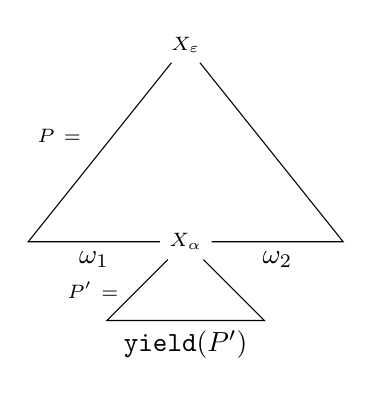
\begin{tikzpicture}
          \node (A) at (0,0) {${\scriptstyle X_\varepsilon}$};
          \coordinate (B) at (-2,-2.5);
          \coordinate (C) at (2,-2.5);
          \node (D) at (0,-2.5) {${\scriptstyle X_\alpha}$};
          \coordinate (E) at (-1,-3.5);
          \coordinate (F) at (1,-3.5);
          
          \draw (A) -- node[above left]{${\scriptstyle P\ =\ }$} (B) -- node[below]{$\omega_1$}(D) -- node[below]{$\omega_2$}(C) -- (A);
          \draw (D) -- node[left]{${\scriptstyle P'\ =\ }$}(E) -- node[below]{$\texttt{yield}(P')$}(F) -- (D);
          
          % \draw [photon] (A) -- node[left]{$\alpha$} (D);
        \end{tikzpicture}
        \caption{$P'' = P \odot P'$}
      \end{subfigure}
      \caption{Конкатенация на дървета}
    \end{figure}
  \end{problem}
  
  Сега да разгледаме частния случай, когато разгледаме $P$ вместо $P'$ в горните условия. Тогава имаме, че $X_\varepsilon = X_\alpha$.
  Дефинираме $n$-тата степен на дървото $P$ по следния начин:
  \begin{itemize}
\item
  $P^{(0)} \df (T_0,\lambda_0)$, където $T_0 = \{\varepsilon\}$ и $\lambda_0(\varepsilon) = \texttt{root}(P)$;
\item
  $P^{(n+1)} \df P^{(n)} \odot P$.
\end{itemize}

\begin{problem}
  Докажете, че $P \odot (P \odot P) = (P \odot P) \odot P$.
\end{problem}


\begin{problem}
  Докажете, че $P^{(n+k)} = P^{(n)} \odot P^{(k)}$.
\end{problem}

\begin{framed}
  \begin{problem}
    \label{prob:tree:iteration}
    Нека $\texttt{yield}(P) = \omega_1 \cdot \texttt{root}(P) \cdot \omega_2$, за някои думи $\omega_1, \omega_2 \in \Sigma^\star$.
    Докажете, че за всяко естествено число $i$ е изпълнено, че:
    \[\texttt{yield}(P^{(i)}) = \omega^i_1 \cdot \texttt{root}(P) \cdot \omega^i_2.\]
  \end{problem}
\end{framed}
\begin{hint}
  Картинката за $i = 2$ изглежда така:

  \begin{figure}[H]
    \begin{subfigure}[t]{0.5\textwidth}
      \centering
      \begin{tikzpicture}
        \coordinate (A) at (0,0);
        \coordinate (B) at (-2,-2.5);
        \coordinate (C) at (2,-2.5);
        \coordinate (D) at (0,-2.5);
        \coordinate (E) at (-2,-5);
        \coordinate (F) at (2,-5);
        \coordinate (G) at (0,-5);
        
        \draw (A) -- node[above left]{$T$} (B) -- (C) -- (A);
        \draw (D) -- node[left]{$T$} (E) -- (F) -- (D);
        
        \draw [photon] (A) -- node[left]{$\alpha$} (D);
        \draw [photon] (D) -- node[left]{$\alpha$} (G);
      \end{tikzpicture}
      \caption{}
    \end{subfigure}
    $\stackrel{\lambda}{\Rightarrow}$
    \begin{subfigure}[t]{0.5\textwidth}
      \centering
      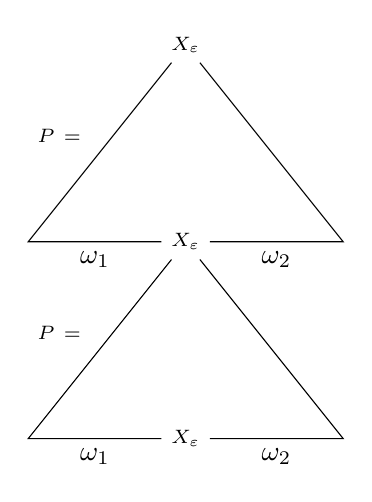
\begin{tikzpicture}
        \node (A) at (0,0) {${\scriptstyle X_\varepsilon}$};
        \coordinate (B) at (-2,-2.5);
        \coordinate (C) at (2,-2.5);
        \node (D) at (0,-2.5) {${\scriptstyle X_\varepsilon}$};
        \coordinate (E) at (-2,-5);
        \coordinate (F) at (2,-5);
        \node (G) at (0,-5) {${\scriptstyle X_\varepsilon}$};
        
        \draw (A) -- node[above left]{${\scriptstyle P\ =\ }$} (B) -- node[below]{$\omega_1$}(D) -- node[below]{$\omega_2$}(C) -- (A);
        \draw (D) -- node[above left]{${\scriptstyle P\ =\ }$}(E) -- node[below]{$\omega_1$} (G) -- node[below]{$\omega_2$} (F) -- (D);
      \end{tikzpicture}
      \caption{$\texttt{yield}(P^{(2)}) = \omega^2_1 \cdot \texttt{root}(P) \cdot \omega^2_2$}
    \end{subfigure}
    \caption{Степенуване на $P$.}
  \end{figure}
\end{hint}

\begin{problem}
  Нека $P = (T,\lambda)$ е дърво на извод съвместимо с граматиката $G$ и нека разгледаме думата $\alpha \in T$.
  % Дефинираме $P \setminus P_\alpha = (T',\lambda')$ по следния начин:
  Дефинираме $\uppercut{P}{\alpha} = (T',\lambda')$ по следния начин:
  \begin{itemize}
  \item
    \mynote{Съобразете, че $\alpha \in \texttt{front}(T')$.}
    $T' = T \setminus \{ \gamma \in T\mid \alpha \prec \gamma\}$, т.е. махаме от $T$ същинските разширения на $\alpha$
  \item
    $\lambda'(\gamma) = \lambda(\gamma)$ за $\gamma \in T'$.
  \end{itemize}
  Докажете, че $\uppercut{P}{\alpha}$ е дърво на извод съвместимо с граматиката $G$ и 
  \[P = (\uppercut{P}{\alpha}) \odot (\lowercut{P}{\alpha}).\]
\end{problem}
\begin{hint}
  Имаме следната картинка:

  \begin{figure}[H]
    \begin{subfigure}[t]{0.5\textwidth}
      \centering
      \begin{tikzpicture}
        \coordinate (A) at (0,0);
        \coordinate (B) at (-2,-2.5);
        \coordinate (C) at (2,-2.5);
        \coordinate (D) at (-0.9,-2.5);
        \coordinate (E) at (0.9,-2.5);
        \coordinate (F) at (0,-1.5);
        
        \coordinate (G) at (0,-2.3);
        \coordinate (H) at (-0.9,-3.3);
        \coordinate (I) at (0.9,-3.3);
        
        \draw (A) -- node[above left]{${\scriptstyle T'\ =\ }$}(B) -- (D) -- (F) -- (E) -- (C) -- (A);
        \draw (G) -- node[left]{${\scriptstyle T_\alpha\ =\ }$} (H) -- (I) -- (G);
        
        \draw [photon] (A) -- node[left]{$\alpha$} (F);
      \end{tikzpicture}
      \caption{$T_\alpha = \alpha^{-1}(T)$}
    \end{subfigure}
    $\stackrel{\lambda}{\Rightarrow}$
    \begin{subfigure}[t]{0.5\textwidth}
      \centering
      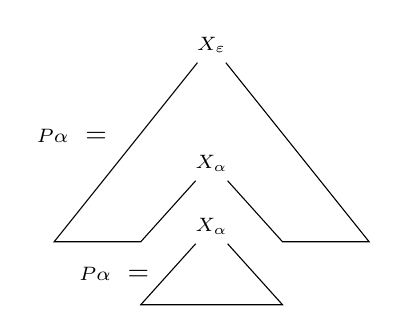
\begin{tikzpicture}
        \node (A) at (0,0) {${\scriptstyle X_\varepsilon}$};
        \coordinate (B) at (-2,-2.5);
        \coordinate (C) at (2,-2.5);
        \coordinate (D) at (-0.9,-2.5);
        \coordinate (E) at (0.9,-2.5);
        \node (F) at (0,-1.5) {${\scriptstyle X_\alpha}$};
        
        \node (G) at (0,-2.3) {${\scriptstyle X_\alpha}$};
        \coordinate (H) at (-0.9,-3.3);
        \coordinate (I) at (0.9,-3.3);
        
        \draw (A) -- node[above left]{${\scriptstyle \uppercut{P}{\alpha}}\ =\ $}(B) -- (D) -- (F) -- (E) -- (C) -- (A);
        \draw (G) -- node[left]{${\scriptstyle \lowercut{P}{\alpha}}\ =\ $} (H) -- (I) -- (G);
      \end{tikzpicture}
      \caption{$\texttt{yield}(\uppercut{P}{\alpha}) = \omega_1 \cdot \texttt{root}(\lowercut{P}{\alpha}) \cdot \omega_2$}
    \end{subfigure}
  \end{figure}
\end{hint}

%%% Local Variables:
%%% mode: latex
%%% TeX-master: "../eai"
%%% End:

\section{Извод върху синтактично дърво}

\mynote{Не знам да има учебник, в който формално да е въведена тази релация. Тя е удобна най-вече за решаване на задачи, както и за доказателството на лемата за покачването.}
\begin{definition}
  За произволна безконтекстна граматика $G$, дефинираме релацията $X \yield{\ell} \alpha$, където $X \in V \cup \Sigma$ и $\alpha \in (V\cup\Sigma)^\star$, по следния начин:
  \begin{important}
    \begin{prooftree}
      \AxiomC{}
      \RightLabel{\scriptsize{правило (0)}}
      \UnaryInfC{$X \yield{0} X$}
    \end{prooftree}
    
    \begin{prooftree}
      \AxiomC{$X \to_G X_1\cdots X_n$}
      \AxiomC{$X_1 \yield{\ell_1} \gamma_1$}
      \AxiomC{$\cdots$}
      \AxiomC{$X_n \yield{\ell_n} \gamma_n$}
      \LeftLabel{\scriptsize{($\ell = \max\{\ell_1,\dots,\ell_n\})$}}
      \RightLabel{\scriptsize{правило (1)}}
      \QuaternaryInfC{$X \yield{\ell+1} \gamma_1\cdots\gamma_n$}
    \end{prooftree}
  \end{important}
\end{definition}

\mynote{ Съобразете, че имаме:
\begin{prooftree}
  \AxiomC{$X \to_G \gamma$}
  \UnaryInfC{$X \yield{1} \gamma$.}
\end{prooftree}
Обърнете внимание също, че тази релация е рефликсивна, но не е транзитивна!}

Да дефинираме $\yield{\star}$ по следния начин:
\[X \yield{\star} \gamma \dff (\exists \ell\in\Nat)[X \yield{\ell} \gamma].\]

\begin{lemma}
  Нека $G$ е безконтекстна граматика, $X \in V \cup \Sigma$ и $\beta \in (V \cup \Sigma)^\star$.
  Тогава ако $X \derive{\star} \beta$, то $X \yield{\star} \beta$.
\end{lemma}  
\begin{proof}
  С пълна индукция по $\ell$ ще докажем, че ако $X \derive{\ell} \beta$, то $X \yield{\star} \beta$.
  \begin{itemize}
  \item
    $\ell = 0$, т.е. $X \derive{0} X$.
    Тогава е ясно, че $X \yield{\star} X$.
  \item
    Нека $\ell > 0$ и $X \derive{\ell} \beta$.
    Според правилата на извод в граматика имаме извода

    \begin{prooftree}
      \AxiomC{$X \to_G X_0X_1\cdots X_k$}
      \AxiomC{$X_0X_1\cdots X_k \derive{\ell-1} \beta$}
      \RightLabel{\scriptsize{правило (1)}}
      \BinaryInfC{$X \derive{\ell} \beta$}
    \end{prooftree}

    \mynote{Естествено, че е възможно някои $X_i$ да са букви от $\Sigma$. Тогава $\beta_i = X_i$ и $X_i \derive{0}_G \beta_i$.}
    Щом имаме, че $X_0X_1\cdots X_k \derive{\ell-1} \beta$, от \Proposition{grammar:divide} знаем, че съществува разбиване на $\beta$ на $k+1$ части, така че:
    \begin{itemize}
    \item
      $\beta = \beta_0 \cdots \beta_{k}$;
    \item
      $X_i \derive{\ell_i} \beta_i$, за всяко $i = 0,\dots,k$;
    \item
      $\ell-1 = \sum^k_{i=1} \ell_i$.
    \end{itemize}
    Понеже $\ell_i < \ell$ за всяко $i = 1,\dots,k$, получаваме следното:
    \begin{prooftree}
      \AxiomC{$X \to_G X_0\cdots X_k$}
      \AxiomC{$X_0 \derive{\ell_0} \beta_0$}
      \RightLabel{\scriptsize{\IndHyp}}
      \UnaryInfC{$X_0 \yield{\star} \beta_0$}
      \AxiomC{$\cdots$}
      \AxiomC{$X_k \derive{\ell_k} \beta_k$}
      \RightLabel{\scriptsize{\IndHyp}}
      \UnaryInfC{$X_k \yield{\star} \beta_k$}
      \RightLabel{\scriptsize{правило (1)}}
      \QuaternaryInfC{$X \yield{\star} \underbrace{\beta_0\cdots\beta_k}_{\beta}$}
    \end{prooftree}
  \end{itemize}
\end{proof}

\begin{lemma}
  Нека $G$ е безконтекстна граматика, $X \in V \cup \Sigma$ и $\gamma \in (V \cup \Sigma)^\star$.
  Тогава ако $X \yield{\star} \gamma$, то $X \derive{\star} \gamma$.
\end{lemma}
\begin{proof}
  С пълна индукция по $\ell$ ще докажем, че ако $X \yield{\ell} \gamma$, то $X \derive{\star} \gamma$.
  \begin{itemize}
  \item
    Нека $\ell = 0$. Това означава, че $X \yield{0} X$. Ясно е, че $X \derive{\star} X$.
  \item
    Нека $\ell > 0$. Тогава имаме следното:
    \begin{prooftree}
      \AxiomC{$X \to_G X_0\cdots X_n$}
      \AxiomC{$X_0 \yield{\ell_0} \gamma_0$}
      \AxiomC{$\cdots$}
      \AxiomC{$X_n \yield{\ell_n} \gamma_n$}
      \RightLabel{\scriptsize{($\ell = 1 + \max\{\ell_0,\dots,\ell_n\})$}}
      \QuaternaryInfC{$X \yield{\ell} \underbrace{\gamma_0\cdots\gamma_n}_{\gamma}$}
    \end{prooftree}
    Понеже $\ell_i < \ell$ за всяко $i = 0,\dots,n$, получаваме следното:
    \begin{prooftree}
      \AxiomC{$X \to_G X_0 \cdots X_{n}$}
      \AxiomC{$X_0 \yield{\ell_0} \gamma_0$}
      \RightLabel{\scriptsize{\IndHyp}}
      \UnaryInfC{$X_0 \derive{\star} \gamma_0$}
      \AxiomC{$\cdots$}
      \AxiomC{$X_n \yield{\ell_n} \gamma_n$}
      \RightLabel{\scriptsize{\IndHyp}}
      \UnaryInfC{$X_n \derive{\star} \gamma_n$}
      \RightLabel{\scriptsize{(\Proposition{unrestricted-grammar:concat})}}
      \TrinaryInfC{$X_0 \cdots X_{n} \derive{\star} \gamma_0\cdots\gamma_{n}$}
      \RightLabel{\scriptsize{правило (1)}}
      \BinaryInfC{$X \derive{\star} \underbrace{\gamma_0\cdots\gamma_{n}}_{\gamma}$}
    \end{prooftree}
  \end{itemize}
\end{proof}

Комбинирайки предишните две леми получаваме следната теорема.
\begin{framed}
  \begin{theorem}\label{th:grammar:yield-derive-equivalent}
    Нека $G$ е безконтекстна граматика, $X \in V \cup \Sigma$ и $\gamma \in (V \cup \Sigma)^\star$.
    Тогава $X \yield{\star} \gamma$ точно тогава, когато $X \derive{\star} \gamma$.
    В частност,
    \[\L(G) = \{\alpha \in \Sigma^\star \mid S \yield{\star}\alpha\}.\]
  \end{theorem}  
\end{framed}

Следващото твърдение ни казва, че има пряка връзка между релацията $\yield{\star}$ и синтактичните дървета.

\begin{important}
  \begin{proposition}\label{pr:yield-relation:parse-tree}
    Нека $G$ е безконтекстна граматика. Тогава
    $X \yield{\ell} \gamma$ точно тогава, когато съществува дърво на извод $P$ съвместимо с $G$, за което
    $\texttt{root}(P) = X$, $\texttt{yield}(P) = \gamma$ и $\texttt{height}(P) = \ell$.
  \end{proposition}
\end{important}
\begin{hint}
  Индукция по $\ell$.
\end{hint}

\begin{extra}
  
  Добре е да обърнем внимание, че е възможно, ако $A \yield{\ell} \alpha$, то да има няколко синтактични дървета с корен променливата $A$,
  които да извеждат думата $\alpha$ и да имат височина $\ell$.
  \begin{example}
    Да разгледаме граматика $G_0$ с правила
    \begin{align*}
      & S \to S + S\ |\ S * S\ |\ (S)\\
      & N \to 0\ |\ 1\ |\ \dots\ |\ 9
    \end{align*}

    В тази граматика нямаме приоритет между $+$ или $*$. Например,
    думата $5 * 6 + 2$ има две различни синтактични дървета $P_1$ и $P_2$, като и двете имат височина $4$ и
    $\texttt{yield}(P_1) = \texttt{yield}(P_2) = 5*6+2$.
    
    \begin{figure}[H]
      \centering
      \qtreecenterfalse
      \Tree [.$S$ [.$S$ [.$N$ $5$ ] ] $*$ [.$S$ [.$S$ [.$N$ $6$ ] ] $+$ [.$S$ [.$N$ $2$ ] ] ] ]
      \hskip 0.6in
      \Tree [.$S$ [.$S$ [.$S$ [.$N$ $5$ ] ] $*$ [.$S$ [.$N$ $6$ ] ] ]  $+$  [.$S$ [.$N$ $2$ ] ] ]
      \caption{Две синтактични дървета в граматиката $G_0$ за думата $5 * 6 + 2$.}
    \end{figure}

    Искаме да модифицираме $G_0$, така че $*$ да има по-висок приоритет спрямо $+$.
    За целта ще разгледаме граматиката $G_1$, която ще поражда същия език като $G_0$, със следните правила:
    \begin{align*}
      & S \to E + S\ |\ E\\
      & E \to N * E\ |\ N\ |\ (S) * E\ |\ (S)\\
      & N \to 0\ |\ 1\ |\ \dots\ |\ 9
    \end{align*}
    Сега думата $5 * 6 + 2$ има само едно дърво на извод.
    \mynote{$*$ има по-висок приоритет от $+$, защото $*$ се среща по-близо до листата.}
    Тук операцията $*$ е с по-висок приоритет в сравнение с операцията $+$.
    \begin{figure}[H]
      \centering
      \Tree [.$S$ [.$E$ [.$N$ $5$ ] $*$ [.$E$ [.$N$ $6$ ] ] ] $+$ [.$S$ [.$E$ [.$N$ $2$ ] ] ] ]
      \caption{Единствено синтактично дърво в граматиката $G_1$ за думата $5 * 6 + 2$.}
    \end{figure}

  \end{example}

% \begin{example}
%   \mynote{Тези примери трябва да се обяснят по-подробно.}
%   Да разгледаме следната граматика:
%   \begin{align*}
%     & S \to \texttt{if } S \texttt{ then } S \texttt{ else }S\ |\ \texttt{ if }S \texttt{ then }S\ |\ C\\
%     & C \to E < E\ |\ E > E\ |\ E == E\ |\ E\\
%     & E \to F + E\ |\ F\\
%     & F \to N * F\ |\ N\ |\ (E) * F\ |\ (E)\\
%     & N \to 0\ |\ 1\ |\ \cdots\ |\ 9
%     \end{align*}

%   Да разгледаме думата
%   \[\texttt{if } x \texttt{ then } \texttt{ if }y \texttt{ then }u\ \texttt{ else }z.\]
%   Имаме многозначност. 
%   Ние искаме следната граматика:
%   \begin{align*}
%     & S \to M\ |\ U\\
%     & M \to \texttt{if } S \texttt{ then } M \texttt{ else }M\ |\ X\\
%     & U \to \texttt{if } S \texttt{ then } S\ |\ \texttt{if } S \texttt{ then } M \texttt{ else }U
%   \end{align*}
% \end{example}

% \begin{example}
%   Да разгледаме граматика с правила
%   \begin{align*}
%     & S \to E\\
%     & E \to E + P\ |\ P\\
%     & P \to P * N\ |\ N\\
%     & N \to (E)\ |\ a.
%   \end{align*}
% \end{example}

\end{extra}

%%% Local Variables:
%%% mode: latex
%%% TeX-master: "../eai"
%%% End:

\newpage
\subsection{Примерни задачи}

\begin{example}
  Езикът $L = \{a^mb^nc^k\mid m+n \geq k\}$ е безконтекстен.
\end{example}  
\begin{proof}
  Да разгледаме граматиката $G$ с правила
  \begin{align*}
    S& \rightarrow aSc\ |\ aS\ |\ B\\
    B& \rightarrow bBc\ |\  bB\ |\ \varepsilon.
  \end{align*}

  От \Proposition{grammar:yield-approximation} имаме, че:
  \begin{align*}
    \L^{\ell+1}_G(S) & = \{a\} \cdot \L^\ell_G(S) \cdot \{c\} \cup \{a\}\cdot \L^\ell_G(S) \cup \L^\ell_G(B)\\
    \L^{\ell+1}_G(B) & = \{b\} \cdot \L^\ell_G(B) \cdot \{c\} \cup \{b\} \cdot \L^\ell_G(B) \cup \{\varepsilon\}.
  \end{align*}

  Да сметнем първите няколко члена на редицата от апроксимации:
  \begin{align*}
    \L^0_G(S) & = \emptyset\\
    \L^0_G(B) & = \emptyset\\
    \L^1_G(S) & = \{a\} \cdot \emptyset \cdot \{c\} \cup \{a\}\cdot\emptyset \cup \emptyset \\
              & = \emptyset\\
    \L^1_G(B) & = \{b\} \cdot \emptyset \cdot \{c\} \cup \{b\} \cdot \emptyset \cup \{\varepsilon\} \\
              & = \{\varepsilon\}\\
    \L^2_G(S) & = \{a\} \cdot \emptyset \cdot \{c\} \cup \{a\}\cdot\emptyset \cup \{\varepsilon\} \\
              & = \{\varepsilon\}\\
    \L^2_G(B) & = \{b\} \cdot \{\varepsilon\} \cdot \{c\} \cup \{b\}\cdot \{\varepsilon\} \cup \{\varepsilon\} \\
              & = \{\varepsilon,b,bc\}\\
    \L^3_G(S) & = \{a\} \cdot \{\varepsilon\} \cdot \{c\} \cup \{a\}\cdot\{\varepsilon\} \cup \{\varepsilon,bc,b\} \\
              & = \{\varepsilon, a, b, ac, bc\}\\
              & = \{a^nb^mc^k \mid 2 > n+m \geq k\}\\
    \L^3_G(B) & = \{b\} \cdot \{\varepsilon,b,bc\} \cdot \{c\} \cup \{b\}\cdot \{\varepsilon,b,bc\} \cup \{\varepsilon,b,bc\} \\
              & = \{\varepsilon,b,bc,bc,bbc,bbcc,bb\}\\
              & = \{ b^mc^k \mid 2 \geq m \geq k\}
  \end{align*}

  Да предположим, че за произволно естествено число $\ell$ е изпълнено следното:
  \begin{align*}
    \L^\ell_G(S) & = \{a^nb^mc^k \mid \ell - 1 > n+m \geq k\}\\
    \L^\ell_G(B)  & = \{ b^mc^k \mid \ell -1 \geq m \geq k\}.
  \end{align*}
  Ще докажем, че
  \begin{align*}
    \L^{\ell+1}_G(S) & = \{a^nb^mc^k \mid \ell > n+m \geq k\}\\
    \L^{\ell+1}_G(B)  & = \{ b^mc^k \mid \ell \geq m \geq k\}.
  \end{align*}

  \begin{itemize}
  \item
    Първо ще докажем, че
    \[\{a^nb^mc^k \mid \ell > n+m \geq k\} \subseteq \L^{\ell+1}_G(S).\]
    Да разгледаме думата $\alpha = a^nb^mc^k$ и $\ell > n+m \geq k$.
    \begin{itemize}
    \item
      Ако $\ell - 1 > n+m$, то от И.П. имаме, че
      \[\alpha \in \L^{\ell}_G(S) \subseteq \L^{\ell+1}_G(S).\]
    \item
      Нека сега $\ell-1 = n+m \geq k$.
      \begin{itemize}
      \item
        Ако $n = 0$, то $\alpha = b^mc^k$ и $\ell-1 = m \geq k$. Тогава от И.П. имаме, че
        \[\alpha \in \L^{\ell}_G(B) \subseteq \L^{\ell+1}_G(S).\]
      \item
        Нека сега $n > 0$. Тогава имаме следните два случая:
        \begin{itemize}
        \item 
          Ако $n + m > k$, то е ясно, че $(n-1) + m \geq k$. От И.П. имаме, че
          \[\alpha \in \{a\} \cdot \L^\ell_G(S) \subseteq \L^{\ell+1}_G(S).\]
        \item
          \mynote{Понеже $n > 0$, то и $k > 0$.}
          Ако $n + m = k$, то е ясно, че $(n-1) + m = k-1$. От И.П. имаме, че
          \[\alpha \in \{a\} \cdot \L^\ell_G(S) \cdot \{c\} \subseteq \L^{\ell+1}_G(S).\]
        \end{itemize}
      \end{itemize}
    \end{itemize}
  \item
    Сега да разгледаме включването
    \[\L^{\ell+1}_G(S) \subseteq \{a^nb^mc^k \mid \ell > n+m \geq k\}.\]
    Да разгледаме произволна дума $\alpha \in \L^{\ell+1}_G(S)$. Имаме четири случая:
    \begin{itemize}
    % \item
    %   Ако $\alpha \in \L^\ell_G(S)$, то от И.П. е ясно, че
    %   \[\alpha \in \{a^nb^mc^k \mid \ell > n+m \geq k\}.\]
    \item
      Ако $\alpha \in \L^\ell_G(B)$, то от И.П. имаме, че
      \[\alpha \in \{b^mc^k \mid \ell > m \geq k\} \subseteq \{a^nb^mc^k \mid \ell > n+m \geq k\}.\]
    \item
      Ако $\alpha \in \{a\} \cdot \L^{\ell}_G(S)$, то от И.П. имаме, че
      \[\alpha \in \{a^{n+1}b^mc^k \mid \ell - 1 > n+m \geq k\} \subseteq \{a^nb^mc^k \mid \ell > n+m \geq k\}.\]
    \item
      Ако $\alpha \in \{a\} \cdot \L^{\ell}_G(S) \cdot \{c\}$, то от И.П. имаме, че
      \[\alpha \in \{a^{n+1}b^mc^{k+1} \mid \ell - 1 > n+m \geq k\} \subseteq \{a^nb^mc^k \mid \ell > n+m \geq k\}.\]
    \end{itemize}
  \end{itemize}

  Сега преминаваме към второто равенство.
  % \[\L^{\ell+1}_G(B) = \L^\ell_G(B) \cup \{b\} \cdot \L^\ell_G(B) \cdot \{c\} \cup \{b\} \cdot \L^\ell_G(B).\]  
  \begin{itemize}
  \item
    Първо ще докажем, че
    \[\{b^mc^k \mid \ell \geq m \geq k\} \subseteq \L^{\ell+1}_G(B).\]
    Да разгледаме думата $\alpha = b^mc^k$ и $\ell \geq m \geq k$.
    \begin{itemize}
    \item
      Ако $m = 0$, то $\alpha = \varepsilon$ и е ясно, че:
      \[\alpha \in \L^{1}_G(B) \subseteq \L^{\ell+1}_G(B).\]
    \item
      Ако $\ell > m$, то от И.П. имаме, че:
      \[\alpha \in \L^{\ell}_G(B) \subseteq \L^{\ell+1}_G(B).\]
    \item
      Нека сега $\ell = m \geq k$.
      \begin{itemize}
      \item
        Ако $\ell = m = k$, то от И.П. имаме, че:
        \[\alpha \in \{a\} \cdot \L^\ell_G(B) \cdot \{c\} \subseteq \L^{\ell+1}_G(B).\]
      \item
        Ако $\ell = m > k$, то от И.П. имаме, че:
        \[\alpha \in \{a\} \cdot \L^\ell_G(B) \subseteq \L^{\ell+1}_G(B).\]
      \end{itemize}
    \end{itemize}
  \item
    Сега да разгледаме включването
    \[\L^{\ell+1}_G(B) \subseteq \{b^mc^k \mid \ell \geq m \geq k\}.\]
    Нека $\alpha \in \L^{\ell+1}_G(B)$. Имаме три случая за $\alpha$.
    \begin{itemize}
    % \item
    %   Нека $\alpha = \L^\ell_G(B)$. Тогава от И.П. е ясно, че:
    %   \[\alpha \in \{b^mc^k \mid \ell-1 \geq m \geq k\} \subseteq \{b^mc^k \mid \ell \geq m \geq k\}.\]
    \item
      Нека $\alpha \in \{b\} \cdot \L^\ell_G(B) \cdot \{c\}$. Тогава от И.П. имаме, че:
      \[\alpha \in \{b^{m+1}c^{k+1} \mid \ell-1\geq m \geq k\} \subseteq \{b^mc^k \mid \ell \geq m \geq k\}.\]
    \item
      Нека $\alpha \in \{b\} \cdot \L^\ell_G(B)$. Тогава от И.П. имаме, че:
      \[\alpha \in \{b^{m+1}c^{k} \mid \ell-1\geq m \geq k\} \subseteq \{b^mc^k \mid \ell \geq m \geq k\}.\]
    \item
      Нека $\alpha \in \{\varepsilon\}$. Тогава е ясно, че имаме:
      \[\alpha \in \{b^mc^l \mid \ell \geq m \geq k\}.\]
    \end{itemize}
  \end{itemize}
  
  
  
  % Лесно се вижда с индукция по $n$, че за всяко $n$ имаме свойствата:
  % % \mynote{\writedown Докажете!}
  % \begin{itemize}
  % \item 
  %   $S \rightarrow^\star_G a^nSc^n$,
  % \item
  %   $S \rightarrow^\star_G a^nS$,
  % \item
  %   $B \rightarrow^\star_G b^nBc^n$,
  % \item
  %   $B \rightarrow^\star_G b^nB$.
  % \end{itemize}
  % Комбинирайки горните свойства, можем да видим, че за всяко $n \geq k$,
  % \begin{itemize}
  % \item 
  %   $S \rightarrow^\star_G a^nSc^k$,
  % \item
  %   $B \rightarrow^\star_G b^nBc^k$.
  % \end{itemize}
  % За да докажем, че $L \subseteq \L(G)$, 
  % да разгледаме една дума $\omega \in L$, т.е. $\omega = a^mb^nc^k$, където $m+n \geq k$.
  % Имаме два случая:
  % \begin{itemize}
  % \item 
  %   $k \leq m$, т.е. $m = k+\ell$ и $m+n = k+\ell+n$.
  %   Тогава имаме изводите:
  %   \[S \rightarrow^\star a^kSc^k,\ S \rightarrow^\star a^\ell S,\ S \rightarrow B,\ B \rightarrow^\star b^nB,\ B \rightarrow \varepsilon.\]
  %   Обединявайки всичко това, получаваме:
  %   \[S \rightarrow^\star a^mb^nc^k.\]
  % \item
  %   $k > m$, т.е. $k = m+\ell$, за някое $\ell > 0$, и $m+n = k+r = m+\ell+r$, за някое $r$.
  %   Тогава имаме изводите:
  %   \[S \rightarrow^\star a^mSc^m,\ S\rightarrow B,\ B\rightarrow^\star b^\ell Bc^\ell,\ B\rightarrow b^rB,\ B\rightarrow\varepsilon,\]
  %   и отново получаваме $S \rightarrow^\star a^mb^nc^k$.
  % \end{itemize}
  % Така доказахме, че $\omega \in \L(G)$.
  
  % Сега ще докажем, че $\L(G) \subseteq L$.
  % С индукция по дължината на извода $l$,
  % ще докажем, че ако $S \stackrel{\ell}{\rightarrow}\omega$, то $\omega \in M$, където
  % \[M = \{a^nSc^k\mid n\geq k\}\cup\{a^nb^mBc^k\mid n+m\geq k\}\cup\{a^nb^mc^k\mid n+m\geq k\}.\]
  
  % Ако $\ell = 0$, то е ясно, че $S \stackrel{0}{\rightarrow} S$ и $S \in M$.

  % Нека $\ell > 0$ и $S \stackrel{\ell-1}{\rightarrow} \alpha \rightarrow \omega$.
  % От {\bf И.П.} имаме, че $\alpha \in M$. Нека $\omega$ се получава от $\alpha$ с прилагане на правилото $C \rightarrow \gamma$.
  % Разглеждаме всички варианти за думата $\alpha \in M$ и за някое правило в граматиката $G$
  % за да докажем, че  $\omega \in M$.
  % Удобно е да представим всички случаи в таблица.
  % \begin{center}
  %   \begin{tabular}{| c | c | c |}
  %     \hline
  %     $\alpha\in M$ & правило в граматиката & $\omega \in M?$ \\ \hline
  %     $a^nSc^k$ & $S \rightarrow aSc$ & $a^{n+1}Sc^{k+1}$ \\ \hline
  %     $a^nSc^k$ & $S \rightarrow aS$ & $a^{n+1}Sc^{k}$ \\ \hline
  %     $a^nSc^k$ & $S \rightarrow B$ & $a^{n}Bc^{k}$ \\ \hline
  %     $a^nb^mBc^k$ & $B \rightarrow bBc$ & $a^nb^{m+1}Bc^{k+1}$\\ \hline
  %     $a^nb^mBc^k$ & $B \rightarrow bB$ & $a^nb^{m+1}Bc^{k}$\\ \hline
  %     $a^nb^mBc^k$ & $B \rightarrow \varepsilon$ & $a^nb^{m}c^{k}$\\ \hline
  %   \end{tabular}
  % \end{center}
  % Във всички случаи се установява, че $\omega \in M$.
  % Сега, за всяка дума $\omega \in L(G)$ следва, че
  % \[\omega \in \Sigma^\star \cap M = \{a^mb^nc^k\mid m+n \geq k\}.\]
\end{proof}

\begin{example}
  Езикът 
  \[L = \{a^nb^mc^kd^\ell \mid n+k = m + \ell\}\]
  е безконтекстен.
\end{example}
\begin{hint}
  Нека $G_1$ е безконтекстна граматика за езика
  \[L_1 = \{a^nb^mc^k \mid m = n+k\},\]
  където правилата на $G_1$ са
  \[S_1 \to AC,\quad  A \to aAb\ |\ \varepsilon,\quad C \to bCc\ |\ \varepsilon.\]
  Нека $G_2$ е безконтекстна граматика за езика 
  \[L_2 = \{b^mc^kd^\ell \mid k = m+\ell\},\]
  където правилата на $G_2$ са
  \[S_2 \to BD,\quad B \to bBc\ |\ \varepsilon,\quad D \to cCd\ |\ \varepsilon.\]
  Тогава граматиката $G$ за $L$ 
  съдържа правилата на граматиките $G_1$ и $G_2$, а също и правилата
  \[S \to aSd\ |\ S_1\ |\ S_2.\]
\end{hint}

\begin{problem}
  \label{prob:equal-but-different}
  \mynote{Ние вече знаем, че този език не е регулярен}
  Езикът
  \[L = \{\alpha\beta \in \{a,b\}^\star \mid\ |\alpha| = |\beta|\ \&\ \alpha \neq \beta\}\]
  е безконтекстен.
\end{problem}
\begin{hint}
  Разгледайте граматиката:
  \begin{align*}
    & S \to AB\ |\ BA\\
    & A \to XAX\ |\ a\\
    & B \to XBX\ |\ b\\
    & X \to a\ |\ b.
  \end{align*}
\end{hint}

\begin{problem}
 Докажете, че езикът
 \[L = \{\alpha \sharp \beta \mid \alpha,\beta \in \{a,b\}^\star\ \&\ \alpha \neq \beta \}\]
 е безконтекстен.
\end{problem}
\begin{hint}
  Разгледайте граматиката:
  \begin{align*}
    & S \to AaR\ |\ BbR\ |\ E\\
    & A \to XAX\ |\ bR\sharp\\
    & B \to XBX\ |\ aR\sharp\\
    & E \to XEX\ |\ XR\sharp\ |\ \sharp XR\\
    & R \to XR\ |\ \varepsilon\\
    & X \to a\ |\ b.
  \end{align*}
  Имаме, че за произволни думи $\alpha,\beta,\gamma,\delta \in \{a,b\}^\star$,
  \begin{align*}
    & S \to^\star \alpha b \gamma \sharp \beta a \delta\ \&\ |\alpha| = |\beta|,\\
    & S \to^\star \alpha a \gamma \sharp \beta b \delta\ \&\ |\alpha| = |\beta|, \text{ или}\\
    & S \to^\star \alpha \sharp \beta\ \&\ |\alpha| \neq |\beta|.
  \end{align*}      
\end{hint}






\begin{problem}
  Докажете, че езикът 
  \[L = \{a^nb^mc^kd^\ell \mid n+k \geq m + \ell\}\]
  е безконтекстен.
\end{problem}

\begin{problem}
  \mynote{
    $S \to aS \mid aSc \mid aB \mid bB$\\
    $B \to bB \mid bBc \mid \varepsilon$
  }
  Докажете, че езикът 
  \[L = \{a^mb^nc^k\mid m+n \geq k + 1\}\]
  е безконтекстен.  
\end{problem}

\begin{problem}
  Докажете, че езикът
  \[L = \{\alpha \sharp \beta \mid \alpha,\beta \in \{a,b\}^\star\ \&\ |\alpha| \neq |\beta| \}\]
  е безконтекстен.
\end{problem}

\begin{problem}
  Да разгледаме граматиката $G$ с правила
  \[S \to AA\ |\ B,\ A \to B\ |\ bb,\ B \to aa\ |\ aB.\]
  Да се намери езика на тази граматика и да се докаже, че граматиката разпознава точно този език.
\end{problem}

%%% Local Variables:
%%% mode: latex
%%% TeX-master: "../eai"
%%% End:

\newpage
\section{Лема за покачването}

\begin{lemma}[за покачването (безконтекстни езици)]
  \index{лема за покачването!безконтекстни езици}
  \label{lem:pumping-context} 
  \marginpar{\cite[стр. 123]{sipser1}, \cite[стр. 125]{hopcroft1}, \cite[стр. 148]{kozen}}
  За всеки безконтекстен език $L$ съществува $p>0$, такова
  че ако $\alpha\in L$, за която $\abs{\alpha} \geq p$, то съществува разбиване на думата на пет части, $\alpha=xyuvw$,
  \marginpar{Ще казваме, че $p$ е константа на покачването}
  за което е изпълнено:
  \begin{enumerate}[1)]
  \item
    $\abs{yv}\geq 1$,
  \item
    $\abs{yuv}\leq p$, и
  \item
    $(\forall i\geq 0)[xy^iuv^iw\in L]$.
\end{enumerate}
\end{lemma}
\begin{proof}
  Нека $G$ е граматиката за езика $L$. Да положим
  \[b = \max\{\ |\gamma| \mid A \to \gamma \text{ е правило в }G\ \}.\]
  Нека
  \[p = b^{\abs{V} + 1}.\]
  Ще покажем, че $p$ е константа на покачването за граматиката $G$.
  
  Да разгледаме произволна дума $\alpha \in \L(G)$, за която $\abs{\alpha} \geq p$.
  Понеже $\L(G)$ е безкраен език, то такива думи съществуват.
  Тогава от \Cor{tree:upper-bound} следва, че ако $P = (T,\lambda)$ е дърво на извод за $\alpha$ в $G$, за което $X_\varepsilon = S$, то
  \[b^{|V| + 1}\leq |\alpha| \leq b^{\texttt{height}(T)}.\]
  Оттук следва, че
  \[|V| + 1 \leq \texttt{height}(T).\]
  Нека измежду всички дървета на извод $P = (T,\lambda)$ за $\alpha$ в граматиката $G$ сме избрали такова с минимална мнощност на $T$.
  Да фиксираме максимален път $\pi$ в $T$, т.е. дума $\pi \in T$ и $|\pi| = \texttt{height}(T)$.
  Ясно е, че
  \marginpar{Броят на върховете по пътя $\pi$ е 1 + броя на ребрата.}
  \[|V| + 1 \leq |\{ X_\gamma \mid \gamma \prec \pi\}| = \texttt{height}(T).\]
  Тук нарочно не броим $X_\pi$, защото $X_\pi \in \Sigma$, а ние се интересуваме само от променливите.
  От принципа на Дирихле следва, че съществува $\beta \prec \pi$, за което
  \begin{equation}
    \label{eq:10}
    X_\beta \in \{X_\gamma \mid \beta \prec \gamma \prec \pi\}.
  \end{equation}
  Нека $\beta$ е най-дългата дума, за която е изпълнено свойството (\ref{eq:10}).
  Да означим с $\gamma$ една от думите, за която $\beta \prec \gamma \prec \pi$ и $X_\gamma = X_\beta$.
  От избора на $\beta$ следва, че
  \begin{equation}
    \label{eq:11}
    \texttt{height}(T_\beta) = |\{ X_\gamma \mid \beta \preceq \gamma \prec \pi\}| \leq |V| + 1,
  \end{equation}
  защото ако допуснем противното, то ще следва, че $|\{ X_\gamma \mid \beta \prec \gamma \prec \pi\}| \geq |V| + 1$ и от принципа на Дирихле ще следва, че
  съществува по-дълга от $\beta$ дума, за която е изпълнено свойството (\ref{eq:10}).
  
  Нека $u = \texttt{yield}(P_\gamma)$. Тогава $yuv = \texttt{yield}(P_\beta)$, за някои думи $y,v \in \Sigma^\star$.
  Това означава, че думата $\alpha$ може да се запише като $\alpha = xyuvw$, за някои $x, w \in \Sigma^\star$.
  % \marginpar{По пътя $\pi$ е възможно да срещнем много различни двойки повтарящи се променливи, ние избрахме възможно най-долната.}
  Освен това имаме свойствата:
  \begin{enumerate}[1)]
  \item
    Да видим първо защо $\abs{yv}\geq 1$.
    Ако допуснем, че $|yv| = 0$, то това означава, че $\alpha = xuw$ и тази дума
    би имала дърво на извод $(P \setminus P_\beta) \odot P_\gamma$, защото:
    \begin{itemize}
    \item 
      $\texttt{yield}(P_\gamma) = u$;
    \item
      $\texttt{yield}(P \setminus P_\beta) = x X_\beta w$;
    \item
      $X_\alpha = X_\beta$.
    \end{itemize}
    Но това противоречи на избора на $P$ като дървото на извод за думата $\alpha$ с минимален брой елементи в $T$.
  \item
    $\abs{yuv} \leq p$, защото $yuv = \texttt{yield}(T_\beta)$ и оттук следва, че:
    \begin{align*}
      \abs{yuv} & \leq b^{\texttt{height}(T_\beta)} & \comment\text{от \Cor{tree:upper-bound}}\\
                & \leq b^{|V|+1} & \comment\text{от (\ref{eq:11})}\\
                & = p
    \end{align*}
  \item
    Остана само да видим защо за всяко естествено число $i$ е изпълнено, че $xy^iuv^iw \in L$.
    Това е най-сложното разсъждение в лемата, затова нека да го разгледаме внимателно.
    Понеже $\beta \prec \gamma$, нека $\rho$ е тази дума, за която $\gamma = \beta \cdot \rho$.
    Ясно е, че $P_\beta\setminus P_\gamma = (P\setminus P_\gamma)_\beta$.
    \begin{itemize}
    \item
      Нека $i = 0$. Тогава $xy^0uv^0w = xuv$ има дърво на извод $(P \setminus P_\beta ) \odot P_\gamma$,
      защото от избора на $\gamma$ и $\beta$ имаме, че:
      \begin{itemize}
      \item 
        $\texttt{yield}(P_\gamma) = u$;
      \item
        $\texttt{yield}(P \setminus P_\beta) = x X_\beta w$;
      \item
        $X_\alpha = X_\beta$.
      \end{itemize}
    \item
      Нека $i = 1$.
      Ясно е от условието, че $xyuvw \in L$, но нека да направим наблюдението, че дървото на извод $P$ за думата $\alpha$ в $G$
      може да се запише и така:
      \[P = (P \setminus P_\beta) \odot (P_\beta \setminus P_\rho) \odot P_\gamma, \]
      защото:
      \begin{itemize}
      \item
        $\texttt{yield}(P\setminus P_\beta) = x X_\beta w$;
      \item
        $\texttt{yield}(P_\beta \setminus P_\rho) = y X_\gamma v$;
      \item
        $\texttt{yield}(P_\gamma) = u$;
      \item
        $X_\beta = X_\gamma$.
      \end{itemize}
      Сега вече имаме идея как да обобщим горната конструкция за $i > 1$.
    \item
      Нека $i > 1$. Тогава $xy^iuv^iw$ има дърво на извод
      \[(P \setminus P_\beta) \odot (P_\beta \setminus P_\rho)^{(i)} \odot P_\gamma,\]
      защото:
      \begin{itemize}
      \item
        $\texttt{yield}(P\setminus P_\beta) = x X_\beta w$;
      \item
        $\texttt{yield}((P_\beta \setminus P_\rho)^{(i)}) = y^i X_\gamma v^i$ от \Prob{tree:iteration};
      \item
        $\texttt{yield}(P_\gamma) = u$;
      \item
        $X_\beta = X_\gamma$.
      \end{itemize}
    \end{itemize}

  \end{enumerate}
\end{proof}

\begin{cor}
  \label{cor:pumping-context-free}
  \marginpar{Ако $L$ е краен език, то е ясно, че $L$ е безконтекстен.}
  Нека $L$ е произволен {\bf безкраен} език. Нека също така е изпълнено, че:
  \begin{description}
  \item[($\forall$)]
    за {\em всяко} естествено число $p \geq 1$,
  \item[($\exists$)]
    можем да намерим дума $\alpha \in L$, $\abs{\alpha}\geq p$, такава че
  \item[($\forall$)]
    за {\em всяко} разбиване на думата на пет части, $\alpha = xyuvw$, със свойствата $\abs{yv} \geq 1$ и $\abs{yuv} \leq p$,
  \item[($\exists$)]
    можем да посочим $i \in \Nat$, за което е изпълнено, че $xy^iuv^iw \not\in L$.
  \end{description}  
  \marginpar{\writedown Докажете! Аналогично е на \Cor{pumping-reg}}
  Тогава $L$ {\bf не} е безконтекстен език.
\end{cor}

\begin{cor}
  \marginpar{\writedown Докажете!}
  Нека $G$ е безконтекстна граматика и $p$ е константата на покачването за $G$.
  Тогава $\abs{\L(G)} = \infty$ точно тогава, когато съществува $\alpha \in \L(G)$, за която $p \leq \abs{\alpha} < 2p$.
\end{cor}
% \begin{proof}
%   Ако съществува дума $\alpha \in L$, за която $\abs{\alpha} \geq p$, то от \Lem{pumping-context} следва,
%   че $\abs{L} = \infty$, защото $\alpha = xyuvw$ и $xy^iuv^iw \in L$, за всяко $i\in\Nat$.

%   За другата посока, нека сега $\abs{L} = \infty$.
%   Да изберем най-късата дума $\alpha \in L$, за която $\abs{\alpha} \geq p$.
%   Ще докажем, че $p \leq \abs{\alpha} < 2p$. За целта да допуснем, че $\abs{\alpha} \geq 2p$.
%   Тогава от \Lem{pumping-context} следва, че $\alpha = xyuvw$, $\abs{yv} \geq 1$, $\abs{yuv} \leq p$, $xy^0uv^0w = xuw \in L$.
%   Ако $\abs{xuw} < p$, то $\abs{yv} > p$, защото $\abs{yv} + \abs{xuw} = \abs{\alpha} \geq 2p$, и следователно $\abs{yuv} > p$, което е противоречие.
%   Следва, че $\abs{\alpha} > \abs{xuw} \geq p$.
%   Получихме, че думата $xuw\in L$ и $\abs{xuw} \geq p$. Това е противоречие с минималността на $\alpha$.
% \end{proof}

% \begin{framed}
%   \Lem{pumping-context} е полезна, когато искаме да докажем, че даден език $L$ {\bf не} е безконтекстен.
%   За целта, доказваме отрицанието на свойствата от \Lem{pumping-context} за $L$, т.е.
%   за всяка константа $p$, ние намираме дума $\alpha \in L$, $\abs{\alpha}\geq p$, такава че за всяко разбиване на думата на пет части, $\alpha = xyuvw$,
%   със свойствата $\abs{yv} \geq 1$ и $\abs{yuv} \leq p$, е изпълнено, че $(\exists i)[xy^iuv^iw \not\in L]$.
% \end{framed}

\begin{remark}
  Алгоритъм за проверка дали един безконтекстен език е безкраен следвайки горния критерий би 
  имал експоненциална сложност относно $|G|$.
\end{remark}

\begin{problem}
  \label{prob:anbncn}
  Докажете, че езикът 
  \[L = \{a^nb^nc^n\ \mid\ n\in\Nat\}\]
  не е безконтекстен.
\end{problem}
\begin{proof}
  \begin{description}
  \item[$(\forall)$]
    Разглеждаме произволна константа $p \geq 1$.
  \item[$(\exists)$]
    Избираме дума $\alpha \in L$, $\abs{\alpha} \geq p$.
    В случая, нека $\alpha = a^pb^pc^p$.
  \item[$(\forall)$]
    Разглеждаме произволно разбиване $xyuvw = \alpha$, за което $\abs{yuv} \leq p$ и $1 \leq \abs{yv}$.
  \item[$(\exists)$]
    Ще изберем $i$, за което $xy^iuv^iw \not\in L$.
    Знаем, че поне едно от $y$ и $v$ не е празната дума.
    Имаме няколко случая за $y$ и $v$.
    \begin{itemize}
    \item
      $y$ и $v$ са думи съставени от една буква.
      В този случай получаваме, че $xy^2uv^2w$ има различен брой букви $a$, $b$ и $c$.
    \item
      $y$ или $v$ е съставена от две букви.
      Тогава е възможно да се окаже, че $xy^2uv^2w$ да има равен брой $a$, $b$ и $c$,
      но тогава редът на буквите е нарушен.
    \item
      понеже $\abs{yuv} \leq p$, то не е възможно в $y$ или $v$ да се срещат и трите букви.
    \end{itemize}  
    Оказа се, че във всички възможни случаи за $y$ и $v$, 
    $xy^2uv^2w \not\in L$.
  \end{description}
  Така от \Cor{pumping-context-free} следва, че езикът $L$ не е безконтекстен.
\end{proof}

\begin{problem}
  Докажете, че езикът
  \[\L(a^\star b^\star c^\star) \setminus \{a^nb^nc^n \mid n \in \Nat\}\]
  е безконтекстен.
\end{problem}

\begin{problem}
  Докажете, че езикът
  \[L = \{a^ib^jc^k\ \mid\ 0 \leq i \leq j \leq k\}\]
  не е безконтекстен.
\end{problem}
\begin{proof}
  \begin{description}
  \item[$(\forall)$]
     Разглеждаме произволна константа $p \geq 1$.
   \item[$(\exists)$]
     Избираме дума $\alpha \in L$, $\abs{\alpha} \geq p$.
     В случая, нека $\alpha = a^pb^pc^p$.
   \item[$(\forall)$]
     Разглеждаме произволно разбиване $xyuvw = \alpha$, за което $\abs{yuv} \leq p$ и $1 \leq \abs{yv}$.
     Знаем, че поне една от $y$ и $v$ не е празната дума.
   \item[$(\exists)$] Ще намерим $i \in \Nat$, за което $xy^iuv^iw \not\in L$.
    \begin{itemize}
    \item
      $y$ и $v$ са съставени от една буква.
      Имаме три случая.
      \begin{enumerate}[i)]
      \item
        $a$ не се среща в $y$ и $v$.
        Тогава $xy^0vu^0w$ съдържа повече $a$ от $b$ или $c$.
      \item
        $b$ не се среща в $y$ и $v$.
        \begin{itemize}
        \item 
          Ако $a$ се среща в $y$ или $v$, тогава $xy^2uv^2w$ съдържа повече $a$ от $b$.
        \item
          Ако $c$ се среща в $y$ или $v$, тогава $xy^0uv^0w$ съдържа по-малко $c$ от $b$.
        \end{itemize}
      \item
        $c$ не се среща в $y$ и $v$.
        Тогава $xy^2uv^2w$ съдържа повече $a$ или $b$ от $c$.
      \end{enumerate}      
     \item
       $y$ или $v$ е съставена от две букви.
       Тук разглеждаме $xy^2uv^2w$ и съобразяваме, че редът на буквите е нарушен.
     \end{itemize}    
   \end{description}
\end{proof}

\begin{problem}
  Докажете, че езикът 
  \[L = \{\ \alpha\alpha\mid \alpha\in \{a,b\}^\star\ \}\]
  не е безконтекстен.
\end{problem}
\begin{hint}
  \begin{itemize}
  \item 
    Защо $\omega = a^pba^pb$ не става ?
  \item
    Защо $\omega = a^pb^{2p}a^p$ не става ?
  \item
    Разгледайте $\omega = a^pb^pa^pb^p$.
  \end{itemize}
\end{hint}

\begin{framed}
  \begin{prop}
    Безконтекстните езици {\bf не} са затворени относно сечение и допълнение.
  \end{prop}
\end{framed}
\begin{hint}
  Да разгледаме езика
  \[L_0 = \{a^nb^nc^n\mid n\in\Nat\},\] за който вече знаем от \Prob{anbncn}, че не е безконтекстен.
  Да вземем също така и безконтекстните езици 
  \marginpar{\writedown Защо са безконтекстни?}
  \[L_1 = \{a^nb^nc^m\mid n,m\in\Nat\},\ L_2 = \{a^mb^nc^n\mid n,m\in\Nat\},\]
  \begin{itemize}
  \item 
    Понеже $L_0 = L_1\cap L_2$, то заключаваме, че безконтекстните езици не са затворени 
    относно операцията сечение.
  \item
    \marginpar{Озн. $\ov{L} = \Sigma^\star \setminus L$}
    Да допуснем, че безконтекстните езици са затворени относно операцията допълнение.
    Тогава  $\ov{L}_1$ и $\ov{L}_2$ са безконтекстни.
    Знаем, че безконтекстните езици са затворени относно обединение. 
    Следователно, езикът $L_3 = \ov{L}_1 \cup \ov{L}_2$ също е безконтекстен.
    Понеже допуснахме, че безконтекстните са затворени относно допълнение, то $\ov{L}_3$ също е безконтекстен.
    Но тогава получаваме, че езикът
    \[L_0 = L_1 \cap L_2 = \ov{\ov{L}_1 \cup \ov{L}_2} = \ov{L}_3\]
    е безконтекстен, което е противоречие.
  \end{itemize}

  Друг пример, с който може да се види, че безконтекстните езици не са затворени относно допълнение е 
  като се докаже, че езикът
  \[\{a,b\}^\star \setminus \{\alpha\alpha\mid \alpha\in \{a,b\}^\star\}\]
  е безконтекстен.
  Това следва лесно като се използва \Prob{equal-but-different}.
\end{hint}

\begin{problem}
  Докажете, че езикът 
  \[L = \{\alpha\beta\alpha^{rev} \mid \alpha,\beta \in \{a,b\}^\star\ \&\ |\alpha| = |\beta|\}\]
  не е безконтекстен.
\end{problem}
\begin{hint}
  \begin{itemize}
  \item
    Защо не става ако разгледаме думата $\alpha = a^pb^pa^p$ ?
  \item 
    Защо не става ако разгледаме думата $\alpha = a^p b^p a^{2p} b^p a^p$ ?
  \item
    Разгледайте $\alpha = a^p b^p a^p b^p b^p a^p$.
    Покачване с повече от $p$ би трябвало да свърши работа.
  \end{itemize}
\end{hint}


\begin{problem}
  Докажете, че езикът 
  \[L = \{\alpha\beta\alpha \mid \alpha,\beta \in \{a,b\}^\star\}\]
  не е безконтекстен.
\end{problem}
\begin{hint}
  \begin{itemize}
  \item 
    Защо не става с $\omega = a^pba^pb$ ?
  \item
    Защо не става с $\omega = ab^pab^p$ ?
  \item
    Пробвайте с $\omega = a^pb^pa^pb^p$.
  \end{itemize}
\end{hint}

% \begin{framed}
%   \begin{prop}
%     Безконтекстните езици {\bf не} са затворени относно сечение и допълнение.
%   \end{prop}
% \end{framed}
% \begin{proof}
%   Да разгледаме езика
%   \[L_0 = \{a^nb^nc^n\mid n\in\Nat\},\] за който вече знаем от \Prob{anbncn}, че не е безконтекстен.
%   Да вземем също така и безконтекстните езици 
%   \marginpar{\writedown Защо са безконтекстни?}
%   \[L_1 = \{a^nb^nc^m\mid n,m\in\Nat\},\ L_2 = \{a^mb^nc^n\mid n,m\in\Nat\},\]
%   \begin{itemize}
%   \item 
%     Понеже $L_0 = L_1\cap L_2$, то заключаваме, че безконтекстните езици не са затворени 
%     относно операцията сечение.
%   \item
%     \marginpar{Озн. $\ov{L} = \Sigma^\star \setminus L$}
%     Да допуснем, че безконтекстните езици са затворени относно операцията допълнение.
%     Тогава  $\ov{L}_1$ и $\ov{L}_2$ са безконтекстни.
%     Знаем, че безконтекстните езици са затворени относно обединение. 
%     Следователно, езикът $L_3 = \ov{L}_1 \cup \ov{L}_2$ също е безконтекстен.
%     Ние допуснахме, че безконтекстните са затворени относно допълнение, следователно $\ov{L}_3$
%     също е безконтекстен.
%     Но тогава получаваме, че езикът
%     \[L_0 = L_1 \cap L_2 = \ov{\ov{L}_1 \cup \ov{L}_2} = \ov{L}_3\]
%     е безконтекстен, което е противоречие.
%   \end{itemize}
% \end{proof}


\begin{problem}
  Докажете, че езикът
  \[L = \{\alpha\sharp\beta \mid \alpha\text{ е подниз на }\beta\}\]
  не е безконтекстен.
\end{problem}
\begin{hint}
  \begin{itemize}
  \item 
    Защо не става ако вземем $\omega = a^p \sharp a^p$ ?
  \item 
    Защо не става ако вземем $\omega = a^pb \sharp a^pb$ ?
  \item
    Разгледайте $\omega = a^pb^p\sharp a^pb^p$.
  \end{itemize}
\end{hint}


\begin{problem}
  Вярно ли е, че следните езици са безконтекстни:
  \begin{enumerate}[a)]
  \item 
    $L = \{\alpha\sharp\beta \mid \alpha,\beta \in \{0,1\}^\star\ \&\ \ov{\alpha}_{(2)} + 1 = \ov{\beta}_{(2)} \}$;
  \item
    $L = \{\alpha\sharp\beta^{rev} \mid \alpha,\beta \in \{0,1\}^\star\ \&\ \ov{\alpha}_{(2)} + 1 = \ov{\beta}_{(2)} \}$ ?
  \end{enumerate}
\end{problem}


%%% Local Variables: 
%%% mode: latex
%%% TeX-master: "../eai"
%%% End: 

\newpage
\subsection{Примерни задачи}

\begin{problem}
  Докажете, че езикът $L = \{a^ib^jc^k\ \mid\ 0 \leq i \leq j \leq k\}$ не е безконтекстен.
\end{problem}
\begin{proof}
  \begin{description}
  \item[$(\forall)$]
     Разглеждаме произволна константа $p \geq 1$.
   \item[$(\exists)$]
     Избираме дума $\alpha \in L$, $\abs{\alpha} \geq p$.
     В случая, нека $\alpha = a^pb^pc^p$.
   \item[$(\forall)$]
     Разглеждаме произволно разбиване $xyuvw = \alpha$, за което $\abs{yuv} \leq p$ и $1 \leq \abs{yv}$.
     Знаем, че поне една от $y$ и $v$ не е празната дума.
   \item[$(\exists)$] Ще намерим $i \in \Nat$, за което $xy^iuv^iw \not\in L$.
    \begin{itemize}
    \item
      $y$ и $v$ са съставени от една буква.
      Имаме три случая.
      \begin{enumerate}[i)]
      \item
        $a$ не се среща в $y$ и $v$.
        Тогава $xy^0vu^0w$ съдържа повече $a$ от $b$ или $c$.
      \item
        $b$ не се среща в $y$ и $v$.
        \begin{itemize}
        \item 
          Ако $a$ се среща в $y$ или $v$, тогава $xy^2uv^2w$ съдържа повече $a$ от $b$.
        \item
          Ако $c$ се среща в $y$ или $v$, тогава $xy^0uv^0w$ съдържа по-малко $c$ от $b$.
        \end{itemize}
      \item
        $c$ не се среща в $y$ и $v$.
        Тогава $xy^2uv^2w$ съдържа повече $a$ или $b$ от $c$.
      \end{enumerate}      
     \item
       $y$ или $v$ е съставена от две букви.
       Тук разглеждаме $xy^2uv^2w$ и съобразяваме, че редът на буквите е нарушен.
     \end{itemize}    
   \end{description}
\end{proof}

\begin{problem}
  Докажете, че езикът 
  \[L = \{\ \alpha\alpha\mid \alpha\in \{a,b\}^\star\ \}\]
  не е безконтекстен.
\end{problem}
\begin{hint}
  \begin{itemize}
  \item 
    Защо $\omega = a^pba^pb$ не става ?
  \item
    Защо $\omega = a^pb^{2p}a^p$ не става ?
  \item
    Разгледайте $\omega = a^pb^pa^pb^p$.
  \end{itemize}
\end{hint}


\begin{problem}
  Докажете, че езикът 
  \[L = \{\alpha\beta\alpha^{\rev} \mid \alpha,\beta \in \{a,b\}^\star\ \&\ |\alpha| = |\beta|\}\]
  не е безконтекстен.
\end{problem}
\begin{hint}
  \begin{itemize}
  \item
    Защо не става ако разгледаме думата $\alpha = a^pb^pa^p$ ?
  \item 
    Защо не става ако разгледаме думата $\alpha = a^p b^p a^{2p} b^p a^p$ ?
  \item
    Разгледайте $\alpha = a^p b^p a^p b^p b^p a^p$.
    Покачване с повече от $p$ би трябвало да свърши работа.
  \end{itemize}
\end{hint}


\begin{problem}
  Докажете, че езикът 
  \[L = \{\alpha\beta\alpha \mid \alpha,\beta \in \{a,b\}^\star\}\]
  не е безконтекстен.
\end{problem}
\begin{hint}
  \begin{itemize}
  \item 
    Защо не става с $\omega = a^pba^pb$ ?
  \item
    Защо не става с $\omega = ab^pab^p$ ?
  \item
    Пробвайте с $\omega = a^pb^pa^pb^p$.
  \end{itemize}
\end{hint}

\begin{problem}
  Докажете, че езикът
  \[L = \{\alpha\sharp\beta \mid \alpha\text{ е подниз на }\beta\}\]
  не е безконтекстен.
\end{problem}
\begin{hint}
  \begin{itemize}
  \item 
    Защо не става ако вземем $\omega = a^p \sharp a^p$ ?
  \item 
    Защо не става ако вземем $\omega = a^pb \sharp a^pb$ ?
  \item
    Разгледайте $\omega = a^pb^p\sharp a^pb^p$.
  \end{itemize}
\end{hint}


\begin{problem}
  Вярно ли е, че следните езици са безконтекстни:
  \begin{enumerate}[a)]
  \item 
    $L = \{\alpha\sharp\beta \mid \alpha,\beta \in \{0,1\}^\star\ \&\ \bin{\alpha} + 1 = \bin{\beta} \}$;
  \item
    $L = \{\alpha\sharp\beta^{\rev} \mid \alpha,\beta \in \{0,1\}^\star\ \&\ \bin{\alpha} + 1 = \bin{\beta} \}$ ?
  \end{enumerate}
\end{problem}

%%% Local Variables:
%%% mode: latex
%%% TeX-master: "../eai"
%%% End:

\newpage
\section{Алгоритми}

Тук ще докажем, че съществуват {\em полиномиални} алгоритми, които за дадена безконтекстна граматика $G$ проверяват:
\begin{itemize}
\item
  дали $\L(G) = \emptyset$;
\item
  дали $|\L(G)| = \infty$;
\item
  дали $|\L(G)| < \infty$;
\item
  по дадена дума $\alpha$ дали $\alpha \in \L(G)$.
\end{itemize}

\subsection{Опростяване на безконтекстни граматики}

\subsubsection*{Премахване на безполезните променливи}

Нека е дадена безконтекстната граматика $G = \CFG$.
\mynote{\cite[стр. 88]{hopcroft1}, \cite[стр. 256]{hopcroft2}.}
Една променлива $A$ се нарича {\bf полезна}, ако съществува извод от следния вид:
\[S \derive{\star}_G \alpha A \beta \derive{\star}_G \gamma,\]
където $\gamma \in \Sigma^\star$, а $\alpha,\beta \in (V \cup \Sigma)^\star$.
Това означава, че една променлива е полезна, ако участва в извода на някоя дума в езика на граматиката.
Една променлива се нарича {\bf безполезна}, ако не е полезна.
Целта ни е да получим еквивалентна граматика $G'$ без безполезни променливи.
Ще решим задачата като разгледаме две леми.

\begin{lemma}
  \label{lem:useless1}
  Нека е дадена безконтекстната граматика $G$ и $\L(G) \neq \emptyset$.
  Съществува алгоритъм, който намира граматика $G'$, за която
  $\L(G) = \L(G')$ и със свойството, че  за всяка променлива $A' \in V'$, съществува дума $\alpha \in \Sigma^\star$,
  за която $A' \derive{\star}_{G'} \alpha$.
\end{lemma}
\begin{hint}
  Целта ни е да намерим множеството $\texttt{Gen}$ от променливи, които генерират думи, т.е. търсим множеството
  \[\texttt{Gen} \df \{A \in V \mid A \yield{\star} \alpha\ \&\ \alpha \in \Sigma^\star \}.\]
  За целта ще построим редица от множества $\texttt{Gen[n]}$ по следния начин:
  \mynote{Всяка итерация на алгоритъма отнема $\mathcal{O}(|G|)$ време. Следователно, изпълнението на целия алгоритъм отнема $\mathcal{O}(|G|^2)$ време.}
  \begin{itemize}
  \item 
    $\texttt{Gen[0]} \df \emptyset$;
  \item
    $\texttt{Gen[n+1]} \df \{A\in V \mid (\exists \alpha \in (\Sigma \cup \texttt{Gen[n]})^\star)[A \to_G \alpha] \}$.
  \item
    Спираме, когато стигнем до такова $n$, за което $\texttt{Gen[n]} = \texttt{Gen[n+1]}$. Лесно се съобразява, че
    $(\forall k \geq n)[\texttt{Gen[n]} = \texttt{Gen[k]}]$.
  \end{itemize}
  Трябва да докажем, че $\texttt{Gen} = \texttt{Gen[n]}$.
  \mynote{\writedown Докажете сами!}
  Това ще направим като докажем, че за всяко $k$, е изпълнена еквивалентността:
  \[A \in \texttt{Gen[k]} \iff (\exists \alpha\in\Sigma^\star)[A \yield{\leq k} \alpha]\]
  Дефинираме $G'$ като $V' = \texttt{Gen[n]}$ и правилата на $G'$ са само тези правила на $G$, в които участват променливи от $V'$ и букви от $\Sigma$.
\end{hint}

\begin{framed}
  \begin{corollary}
    Съществува {\em полиномиален} алгоритъм, който определя за всяка безконтекстна граматика $G$ дали $\L(G) = \emptyset$.
  \end{corollary}  
\end{framed}
\begin{proof}
  Прилагаме алгоритъма от \Lemma{useless1} и намираме множеството от променливи $V'$.
  Тогава $\L(G) = \emptyset$ точно тогава, когато $S \not\in V'$.  
\end{proof}

\begin{lemma}
  \label{lem:useless2}
  Съществува алгоритъм, който по дадена безконтекстна граматика $G = \CFG$, намира $G' = \pair{V',\Sigma,S,R'}$, $\L(G') = \L(G)$,
  със свойството, че за всяко $X \in V'$ съществуват $\alpha, \beta \in (V'\cup\Sigma)^\star$,
  за които $S \derive{\star} \alpha X \beta$,
  т.е. всяка променлива в $G'$ е достижима от началната променлива $S$.
\end{lemma}
\begin{hint}
  Нашата цел е да намерим множеството
  \[\texttt{Reach} \df \{B \in V \mid S \yield{\star} \alpha B \beta\text{, за някои }\alpha,\beta \in (\Sigma \cup V)^\star\}.\]
  Новата граматика $G'$ ще има променливи $V' \df \texttt{Reach}$,
  като правилата на граматика $G'$ са същите като тези на $G$, но ограничени до $V'$.
  Лесно се доказава, че $\L(G) = \L(G')$.
  Остава да намерим множеството $\texttt{Reach}$.
  За да постигнем тази цел, ще започнем да строим множествата $\texttt{Reach[i]} \subseteq V$ по следния начин:
  \begin{align*}
    \texttt{Reach[0]} \df & \{S\}\\
    % \texttt{Reach[i+1]}
    % \df & \{ B \in V \mid (\exists A \in \texttt{Reach[i]})[ A \to_G \alpha B \beta\text{, за някои }\alpha,\beta \in (V \cup \Sigma)^\star]\}\\
                        %   & \cup \texttt{Reach[i]}\\
                         % \df & \{ B \in V \mid (\exists A \in \texttt{Reach[i]})[ A \yield{\leq 1} \alpha B \beta\text{, за някои }\alpha,\beta \in (V \cup \Sigma)^\star]\},
  % \end{align*}
  % което може да се запише и така:
  % \begin{align*}
    \texttt{Reach[i+1]} \df & \{ B \in V \mid (\exists A \in \texttt{Reach[i]})[ A \to_G \alpha B \beta\text{, за някои }\alpha,\beta \in (V \cup \Sigma)^\star]\}\\
                            & \cup \texttt{Reach[i]}.    
  \end{align*}
  Докажете, че за всяко $i$ е изпълнено:
  \[\texttt{Reach[i]} = \{B \in V \mid S \yield{\leq i} \alpha B \beta\text{, за някои }\alpha,\beta \in (\Sigma \cup V)^\star\}.\]
  \mynote{\writedown Защо сме сигурни, че ще достигнем такава стъпка?}
  Спираме да строим тези множества, когато достигнем до стъпка $n$, за която
  \[\texttt{Reach[n]} = \texttt{Reach[n+1]}.\]
  Съобразете, че за това $n$ е изпълнено, че $\texttt{Reach[n]} = \texttt{Reach}$, т.е.
  \[\texttt{Reach[n]} = \{B \in V \mid S \yield{\star} \alpha B \beta\text{, за някои }\alpha,\beta \in (\Sigma \cup V)^\star\}.\]
\end{hint}

\begin{extra2}
  \begin{example}
    Да разгледаме безконтекстната граматика $G$ с правила:
    \begin{align*}
      & S \to AB\ |\ aA\\
      & A \to a\ |\ aAa\\
      & B \to SB\ |\ BC\\
      & C \to \varepsilon\ |\ cC.
    \end{align*}
    Първо да намерим променливите, от които се извеждат думи.
    \begin{itemize}
    \item
      $\texttt{Gen[0]} = \emptyset$;
    \item 
      $\texttt{Gen[1]} = \{A, C\}$, защото $A \to a$ и $C \to \varepsilon$;
    \item
      $\texttt{Gen[2]} = \{A, C, S\}$, защото $S \to aA$;
    \item
      не можем да добавим $B$ към $\texttt{Gen[3]}$, следователно $\texttt{Gen[3]} = \texttt{Gen[2]}$.
    \end{itemize}
    Получаваме граматиката $G'$:
    \begin{align*}
      & S \to aA\\
      & A \to a\ |\ aAa\\
      & C \to \varepsilon\ |\ cC.
    \end{align*}
    Сега премахваме променливите и буквите, които не са достижими от началната промелива $S$.
    \begin{itemize}
    \item
      $\texttt{Reach[0]} = \{S\}$;
    \item
      $\texttt{Reach[1]} = \{S,A\}$, защото $S \to aAa$;
    \item
      $\texttt{Reach[2]} = \{S,A\}$.
    \end{itemize}
    Така получаваме граматиката $G''$ със следните правила:
    \begin{align*}
      & S \to aA\\
      & A \to a\ |\ aAa.
    \end{align*}
  \end{example}
\end{extra2}

\begin{theorem}
  За всяка безконтекстна граматика $G$, за която $\L(G) \neq \emptyset$, съществува еквивалетнтна на нея безконтекстна граматика $G'$ без безполезни правила.
  Освен това, граматиката $G'$ може да се намери за полиномиално време.
\end{theorem}
\begin{hint}
  \mynote{\writedown Защо е важна последователността на прилагане? Например, да разгледаме граматиката
    \begin{align*}
      & S \to AB\ |\ ab\\
      & A \to aA\ |\ \varepsilon\\
      & B \to bB.      
    \end{align*}
    Ако първо приложим процедурата от \Lemma{useless2}, то нищо няма да премахнем, защото $A$ и $B$ са достижими от $S$.
    След това, ако приложим процедурата от \Lemma{useless1}, то ще премахнем всички правила, в които участва $B$.
    Така $A$ става недостижима от $S$ и трябва пак да приложим процедурата от \Lemma{useless2}.
    Алгоритъмът описан тук е квадратичен. Има и линеен такъв. Вижте \cite[стр. 296]{hopcroft2}}
  Прилагаме върху $G$ първо процедурата от \Lemma{useless1} и след това върху резултата прилагаме процедурата от \Lemma{useless2}.
\end{hint}

\begin{extra}
  \begin{problem}
    Проверете дали $\L(G) = \emptyset$, където правилата на $G$ са:
    \begin{align*}
      & S \to AS\ |\ BC\\
      & A \to a\ |\ BA\ |\ SB\\
      & B \to b\ |\ BC\ |\ AB\\
      & C \to CB\ |\ SC\ |\ AS.
    \end{align*}
  \end{problem}
  % \begin{hint}
  %   Лесно се проверява, че:
  %   \begin{align*}
  %     \texttt{Gen[1]} & = \{A,B\}\\
  %     \texttt{Gen[2]} & = \{A,B\}.
  %   \end{align*}
  % \end{hint}
\end{extra}

%%% Local Variables:
%%% mode: latex
%%% TeX-master: "../eai"
%%% End:


\subsubsection*{Премахване на $\varepsilon$-правила}
\index{$\varepsilon$-правила}

\begin{lemma}
  Съществува {\em експоненциален} алгоритъм, такъв че превръща всяка безконтекстна граматика $G$ в безконтекстна граматика $G'$ без правила от вида $A \to \varepsilon$,
  и $\L(G') = \L(G) \setminus \{\varepsilon\}$.
\end{lemma}
\begin{hint}
  За да премахнем правилата от вида $A \to \varepsilon$ от граматиката, първо трябва да намерим множеството
  от променливи
  \[\texttt{E} = \{A \in V \mid A \yield{\star} \varepsilon\}.\]
  За да направим това, следваме процедурата:
  \begin{enumerate}[1)]
  \item 
    \mynote{На всяка стъпка трябва да обходим цялата граматика, следователно всяка итерация отнема $\mathcal{O}(|G|)$ време.}
    Първо % трябва да намерим множеството
    % \[\texttt{E} = \{A \in V \mid A \yield{\star}_G \varepsilon\}.\]
    % Това правим като
    строим множествата $\texttt{E[n]}$ по следния начин:
    \begin{itemize}[-]
    \item
      $\texttt{E[0]} \df \emptyset$;
    \item
      \mynote{Обърнете внимание, че имаме $\texttt{E[n]}^\star$, а
        не просто $\texttt{E[n]}$. Също така да напомним, че $\emptyset^\star = \{\varepsilon\}$.}
      $\texttt{E[n+1]} \df \{ B \in V \mid (\exists \alpha \in \texttt{E[n]}^\star)[B \to_G \alpha ]\}$.
    \item
      Докажете, че за всяко $n$ е изпълнено, че
      \[\texttt{E[n]} = \{A \in V \mid A \yield{\leq n} \varepsilon\}.\]
    %   $A \in \texttt{E[n]}$ точно тогава, когато съществува дърво на извод $P$, за което
    % $A = \texttt{root}(P)$, $\texttt{yield}(P) = \varepsilon$ и $\texttt{height}(P) \leq n$.
    \item
      \mynote{Намираме $\texttt{E}$ за време $\mathcal{O}(|G|^2)$.}
      Спираме на първото $n$, за което $\texttt{E[n]} = \texttt{E[n+1]}$.
      Лесно се съобразява, че за това $n$ е изпълнено, че
      \[\texttt{E[n]} = \{A \in V \mid A \yield{\star} \varepsilon\}.\]
    \end{itemize}
  \item
    Строим множеството от правила $R'$, в което няма $\varepsilon$-правила по следния начин.
    За всяко правило $A \to_G X_1\cdots X_k$,
    добавяме към $R'$ всички правила от вида $A \to_G Y_1\cdots Y_k$, където:
    \mynote{Броят на правилата може да се увеличи експоненциално, защото в най-лошия случай извеждаме всички подмножества на дадено множество от променливи}
    \begin{itemize}[-]
    \item 
      ако $X_i \not\in \texttt{E}$, то $Y_i = X_i$;
    \item
      ако $X_i \in \texttt{E}$, то $Y_i = X_i$ или $Y_i = \varepsilon$;
    \item
      не всички $Y_i$ са $\varepsilon$.
    \end{itemize}
    \mynote{\writedown Докажете сами!}
    Лесно се съобразява, че $\L(G') = \L(G) \setminus \{\varepsilon\}$.
    % \begin{itemize}
    % \item
    %   Нека $A \stackrel{l}{\to_G} \omega$ за $\omega \neq \varepsilon$. Тогава $A \to^\star_{G'} \omega$.
    % \item
    %   Нека $A \stackrel{l}{\to_{G'}} \omega$ за $\omega \neq \varepsilon$. Тогава $A \to^\star_{G} \omega$.
    % \end{itemize}
  \end{enumerate}
\end{hint}

\begin{extra2}
  \begin{example}
  Нека е дадена граматиката $G$ с правила
  \begin{align*}
    & S \to D\\
    & D \to AD\ |\ b\\
    & A \to AB\ |\ BC\ |\ a\\
    & B \to AA\ |\ UC\\
    & C \to \varepsilon\ |\ CA\ |\ a\\
    & U \to \varepsilon\ |\ aUb.
  \end{align*}

  Тогава
  \begin{itemize}[-]
  \item
    $\texttt{E[0]} = \emptyset$;
  \item
    $\texttt{E[1]} = \{C,U\}$;
  \item
    $\texttt{E[2]} = \{C,U,B\}$;
  \item
    $\texttt{E[3]} = \{C,U,B,A\}$;
  \item
    $\texttt{E[4]} = \texttt{E[3]}$. Следователно,
    \[\texttt{E} = \{X \in V \mid X \yield{\star} \varepsilon\} = \{C,U,B,A\}.\]
  \end{itemize}
  
  Това означава, че $\varepsilon \not\in \L(G)$.
  Граматиката $G'$ без $\varepsilon$-правила, за която $\L(G') = \L(G)$ има следните правила
  \begin{align*}
    & S \to D \\
    & D\to AD\ |\ D\ |\ b \\
    & A \to A\ |\ B\ |\ C\ |\ AB\ |\ BC\ |\ a \\
    & B\to A\ |\ C\ |\ AA\ |\ U\ |\ UC\\
    & C \to C\ |\ A\ |\ CA\ |\ a\\
    & U \to aUb\ |\ ab.
  \end{align*}
\end{example}  
\end{extra2}

%%% Local Variables:
%%% mode: latex
%%% TeX-master: "../eai"
%%% End:


\subsubsection*{Премахване на преименуващи правила}
\index{преименуващи правила}
\mynote{В \cite[стр. 263]{hopcroft2} преименуващите правила се наричат \emph{unit productions}.}
Едно правило в граматиката $G$ се нарича {\bf преименуващо}, ако е от вида $A \to B$.
Нека е дадена граматика $G = \CFG$.
Ще построим еквивалентна граматика $G'$ без преименуващи правила.
В началото нека в $G'$ да добавим всички правила от $G$, които не са преименуващи.
След това, за всякa променлива $A$, за която $A \derive{\star}_G B$,
ако $B \to \alpha$ е правило в граматиката $G$, което не е преименуващо,
то добавяме към $G'$ правилото $A \to \alpha$.

\begin{lemma}
  Нека $G$ е безконтекстна граматика без $\varepsilon$-правила.
  Съществува {\em полиномиален} алгоритъм, такъв че превръща всяка безконтекстна граматика $G$ в безконтекстна граматика $G'$ без преименуващи правила
  и $\L(G') = \L(G) \setminus \{\varepsilon\}$.
\end{lemma}
\begin{hint}
  Първо намираме множеството от двойки
  \[\texttt{Ren} = \{(A,B) \in V\times V \mid A \derive{\star} B\}\]
  като строим множествата по такъв начин, че да е изпълнено свойството:
  \[\texttt{Ren[n]} = \{(A,B) \in V\times V \mid A \derive{\leq n} B\}\]

  \begin{align*}
    & \texttt{Ren[0]} \df \{(A,A) \mid A \in V\}\\
    & \texttt{Ren[n+1]} \df \texttt{Ren[n]} \cup \{(A,B) \mid (\exists C)[ A \to_G C\ \&\ (C,B) \in \texttt{Ren[n]}]\}.
  \end{align*}
  
  % \begin{itemize}
  % \item
  %   % Ясно е, че $\texttt{Ren[0]} \df \{(A,A) \mid A \in V\}$.
  %   $
  % \item
  %   Нека имаме $\texttt{Ren[n]}$. Тогава дефинираме
  %   \mynote{Всяка итерация отнема $\mathcal{O}(|G|)$ време.}
  %   \[\texttt{Ren[n+1]} \df \texttt{Ren[n]} \cup \{(A,B) \mid (\exists C)[ A \to_G C\ \&\ (C,B) \in \texttt{Ren[n]}]\}.\]
  % \item
  \mynote{$|\texttt{Ren}|$ има големина $\mathcal{O}(|G|^2)$.}
  Спираме на първото $n$, за което $\texttt{Ren[n]} = \texttt{Ren[n+1]}$. Тогава $\texttt{Ren} = \texttt{Ren[n]}$.
  % \end{itemize}
  
  Нека $R'_0 \df R \setminus (V\times V)$ са правилата на $R$, които не са преименуващи. Тогава
  \[R' \df  \{\ (A,\alpha) \in V \times (V\cup\Sigma)^\star \mid (\exists B)[(A,B) \in \texttt{Ren}\ \&\ (B,\alpha) \in R'_0]\ \}.\]
\end{hint}

% \ExtraMaterial{
\begin{extra}
\begin{multicols}{2}
    \begin{example}
      Нека е дадена граматиката $G$ с правила  
      \begin{align*}
        & S \to B\ |\ CC\ |\ b\\
        & A \to S\ |\ SB\\
        & B \to C\ |\ BC\\
        & C \to AB\ |\ a\ |\ b.
      \end{align*}
      Да намерим първо множеството $\texttt{Ren}$.
      \begin{align*}
        \texttt{Ren[0]} = \{ & (S,S), (A,A), (B,B), (C,C)\};\\
        \texttt{Ren[1]} = \{ & (S,S), (S,B), (A,A), (A,S),\\
                             & (B,B), (B,C), (C,C)\};\\
        \texttt{Ren[2]} = \{ & (S,S),(S,B), (S,C), (B,B),\\
                             & (B,C), (C,C), (A,A), (A,S),\\
                             & (A,B)\};\\
        \texttt{Ren[3]} = \{ & (S,S),(S,B), (S,C), (B,B),\\
                             & (B,C), (C,C), (A,A), (A,S),\\
                             & (A,B), (A,C)\};\\
        \texttt{Ren[4]} = \{ & (S,S),(S,B), (S,C), (B,B),\\
                             & (B,C), (C,C), (A,A), (A,S),\\
                             & (A,B), (A,C)\}.
      \end{align*}
      
      Получихме, че $\texttt{Ren[3]} = \texttt{Ren[4]}$.
      Оттук можем да заключим следното:
      \begin{align*}
        & A \derive{\star} A,B,S,C\\
        & B \derive{\star} B,C\\
        & S \derive{\star} S,B,C\\
        & C \derive{\star} C.          
      \end{align*}
      % \end{itemize}
      
      Първо добавяме към $R'$ правилата, които не са преименуващи, а именно:
      \begin{align*}
        & A \to SB\\
        & B \to BC\\
        & C \to AB\ |\ a\ |\ b\\
        & S \to CC\ |\ b.
      \end{align*}
      \begin{itemize}
      \item 
        Понеже имаме,че $A \derive{\star} B,S,C$, то добавяме към $R'$ правилата:
        \[A \to BC\ |\ AB\ |\ a\ |\ b\ |\ CC.\]
      \item
        Понеже имаме,че $B \derive{\star}_G C$, то добавяме към $R'$ правилата:
        \[B \to AB\ |\ a\ |\ b.\]
      \item
        Понеже имаме, че $S \derive{\star}_G B,C$, то добавяме към $R'$ правилата:
        \[S \to BC\ |\ AB\ |\ a\ |\ b.\]
      \end{itemize}
      Накрая получаваме, че граматиката $G'$ има правила
      \begin{align*}
        & S \to BC\ |\ AB\ |\ CC\ |\ a\ |\ b\\
        & A \to BS\ |\ BC\ |\ AB\ |\ a\ |\ b\ |\ CC\\
        & B \to AB\ |\ a\ |\ b\ |\ BC\\
        & C \to AB\ |\ a\ |\ b.
      \end{align*}
    \end{example}
  \end{multicols}
\end{extra}

\begin{extra}
\begin{problem}
  Премахнете преименуващите правила от граматиката $G$, като запазите езика, ако $G$ има следните правила:
    \begin{align*}
      & S \to C\ |\ CC\ |\ b\\
      & A \to B\\
      & B \to S\ |\ C\ |\ BC\\
      & C \to a\ |\ AB;
    \end{align*}
\end{problem}
\end{extra}

%%% Local Variables:
%%% mode: latex
%%% TeX-master: "../eai"
%%% End:


\subsubsection*{Премахване на дългите правила}

Едно правило се нарича дълго, ако е от вида $A \to \beta$, където $|\beta| \geq 3$.
Да разгледаме едно дълго правило в граматиката от вида $A \to x_1x_2\cdots x_k$, 
където $k \geq 3$ и $x_i \in V \cup \Sigma$. За да получим еквивалентна граматика без това дълго правило,
добавяме нови променливи $A_1,\dots, A_{k-2}$, и правила
\[A \to x_1A_1,\ A_1 \to x_2A_2, \dots,\ A_{k-2} \to x_{k-1}x_k.\]


\begin{problem}
  Нека е дадена граматиката  $G = \pair{\{S,A,B,C\}, \{a,b\}, S, R}$.
  Използвайте обща конструкция, за да премахнете ,,дългите'' правила от $ G$ като при това получите 
  безконтестна граматика $G_1$ с език $\L(G) = \L(G_1)$, където правилата на граматиката са:
  % \begin{enumerate}[a)]
  % \item
  %   \begin{align*}
  %     & S \to \varepsilon\ |\ ab\ |\ aAba\\
  %     & A\to aBCb\\
  %     & B\to bbb\\
  %     & C\to aC\ |\ aCaC;
  %   \end{align*}
  % \item
    \begin{align*}
      & S\to CC\ |\ b\\
      & A\to BSB\ |\ a\\
      & B\to ba\ |\ BC\\
      & C\to BaSA\ |\ a\ |\ b.
    \end{align*}
  % \end{enumerate}
\end{problem}

%%% Local Variables:
%%% mode: latex
%%% TeX-master: "../eai"
%%% End:


\subsection{Нормална Форма на Чомски}
\index{Чомски}
%[стр. 99 от \cite{sipser}]
\index{нормална форма на Чомски}
Една безконтекстна граматика е в {\bf нормална форма на Чомски}, ако
всяко правило е от вида
\[A \rightarrow BC\mbox{ и }A \rightarrow a,\]
като $A, B, C$.
\mynote{Ако искаме $\varepsilon$ да бъде в езика на граматиката, то добавяме нова начална променлива $S_0$ и правило $S_0 \to_G \varepsilon$.}
% Освен това, позволяваме правилото $S\to\varepsilon$.
% \footnote{В \cite[стр. 151]{papadimitriou} дефиницията е малко по-различна.
% Там дефинират $G$ да бъде в нормална форма на Чомски ако $R \subseteq V\times(V\cup\Sigma)^2$.
% В този случай губим езиците $\{\varepsilon\}$ и $\{a\}$, за $a\in\Sigma$.}

\begin{framed}
  \begin{theorem}
    Всеки безконтекстен език $L$, който не съдържа $\varepsilon$, се поражда от безконтекстна граматика в нормална форма на Чомски.
  \end{theorem}
\end{framed}
\begin{proof}
%  \marginpar{Броят на правилата може да се увеличи експоненциално.}
  Нека имаме безконтекстна граматика $G$, за която $L = \L(G)$.
  Ще построим безконтекстна граматика $G^\prime$ в нормална форма на Чомски, $L = \L(G^\prime)$.
  % [стр. 99 от \cite{sipser}]
  Следваме следната процедура:
  \begin{itemize}
  % \item
  %   Добавяме нов начален символ $S_0$ и правило $S_0 \to S$.
  \item
    Премахваме дългите правила.
    Това можем да направим за време $\mathcal{O}(|G|)$
    като новата граматика ще има дължина $\mathcal{O}(|G|)$.
  \item
    \mynote{Важно е, че преди това сме премахнали дългите правила. Вижте \cite[стр. 296]{hopcroft2}.}
    Премахваме $\varepsilon$-правилата.
    Това можем да направим за време $\mathcal{O}(|G|^2)$
    като новата граматика ще има дължина $\mathcal{O}(|G|)$.
  \item
    Премахваме преименуващите правила.
    Това можем да направим за време $\mathcal{O}(|G|^2)$
    като новата граматика ще има дължина $\mathcal{O}(|G|^2)$.
  \item
    За правила от вида $A\to u_1 u_2$, където $u_1, u_2 \in V \cup \Sigma$, 
    заменяме всяка буква $u_i$ с новата променлива $U_i$
    и добавяме правилото $U_i\to u_i$.
    Например, правилото $A \to aB$ се заменя с правилото $A \to XB$ и добавяме правилото $X \to a$,
    където $X$ е нова променлива.
    Това можем да направим за време $\mathcal{O}(|G|)$ и новата граматика ще има дължина $\mathcal{O}(|G|)$.
  \item
    Ако искаме $\varepsilon$ да бъде в езика на граматиката, то добавяме нова начална променлива $S_0$
    и правило $S_0 \to_G \varepsilon$.
  \end{itemize}
\end{proof}

\begin{theorem}
  При дадена безконтекстна граматика $G$, можем да намерим еквивалентна
  на нея граматика $G'$ в нормална форма на Чомски за време $\mathcal{O}(|G|^2)$,
  като получената граматика е с дължина $\mathcal{O}(|G|^2)$.
\end{theorem}

\begin{theorem}
  \mynote{\cite[стр. 137]{hopcroft1}. Важно е, че алгоритмите са полиномиални. От \Lemma{pumping-context} имаме експоненциални алгоритми.}
  Съществуват \emph{полиномиални} алгоритми, които определят по дадена безконтекстна граматика $G$ дали:
  \begin{enumerate}[a)]
  \item
    $\abs{\L(G)} < \infty$;
  \item
    $\abs{\L(G)} = \infty$.
  \end{enumerate}
\end{theorem}
\begin{proof}
  Нека е дадена една безконтекстна граматика $G$.
  Нека да разгледаме граматиката $G'$ в НФЧ {\em без безполезни променливи}, за която $\L(G) = \L(G')$.
  От граматиката $G' = \pair{V',\Sigma,S,R'}$ строим граф с възли променливите от $V'$ като
  за $A,B \in V'$ имаме ребро $A \to B$ точно тогава, когато съществува $C \in V'$,
  за което $A \to BC$ или $A \to CB$ е правило в $R'$.
  Сега ще съобразим, че ако в получения граф имаме цикъл, то $\L(G') = \infty$.

  Да разгледаме един такъв цикъл в графа:
  \[A_0 \to A_1 \to A_2 \to \cdots \to A_n \to A_0.\]
  Това означава, че 
  \[A_0 \derive{1}_G \alpha_1 A_1 \beta_1 \derive{1}_G \alpha_2 A_2 \beta_2 \derive{1}_G \cdots \derive{1}_G \alpha_n A_n \beta_n \derive{1}_G \alpha_{n+1} A_0 \beta_{n+1}.\]
  Понеже граматиката е в НФЧ имаме, че $|\alpha_i\beta_i| = i$.
  Понеже няма безполезни символи в граматика и тя е в НФЧ следва, че съществуват думи $\omega,\rho \in \Sigma^\star$, за които $\alpha_{n+1} \derive{\star} \omega$ и $\beta_{n+1} \derive{\star} \rho$,
  където $|\omega\rho| \geq n+1$, защото $|\alpha_{n+1}\beta_{n+1}| = n+1$.
  Понеже няма безполезни символи в граматиката, то съществуват $\delta, \gamma \in \Sigma^\star$, за които
  $S \derive{\star} \delta  A_0 \gamma$. Получаваме:
  \[ S \derive{\star}_G \delta A_0 \gamma \derive{\star}_G \delta \alpha_{n+1} A_0 \beta_{n+1} \gamma \derive{\star}_G \delta \omega A_0 \rho\gamma \derive{\star}_G \cdots \derive{\star}_G \delta \omega^i A_0 \rho^i \gamma \derive{\star}_G \delta\omega^i\alpha\rho^i\gamma,\]
  където $A_0 \derive{\star}_G \alpha$, за някое $\alpha \in \Sigma^\star$.

  Ако в графът няма цикли, то езикът $\L(G)$ е краен, защото ако от променливата $A$ най-дългият път има дължина $k+1$,
  то за променливите $B$ и $C$, за които имаме правилото $A\to BC$, най-дългият път от $B$ и $C$ има дължина най-много $k$.

  Ако най-дългият път от $A$ има дължина $k$, то всяко дърво на извод $P$, за което $\texttt{root}(P) = A$ и $\texttt{yield}(P) \in \Sigma^\star$,
  е такова, че $\texttt{height}(P) \leq k$. От \Corollary{tree:upper-bound} следва, че всички думи, които се извеждат от $A$ са най-много $2^{k}$ на брой,
  защото всяко такова дърво на извод е двоично и $\texttt{yield}(P) \leq 2^k$.
\end{proof}

%%% Local Variables:
%%% mode: latex
%%% TeX-master: "../eai"
%%% End:


\subsection{Проблемът за принадлежност}

\begin{theorem}
  Съществува {\em полиномиален} алгоритъм относно дължината на входната дума, който проверява дали дадена дума принадлежни на граматиката $G$.
\end{theorem}
% \begin{proof}[стр. 154 от \cite{papadimitriou}]
Можем да приемем, че $G = \CFG$ е граматика в нормална форма на Чомски.
% Нека $\alpha = a_0a_1\dots a_{n-1}$ е дума, за която искаме да проверим дали $\alpha \in \L(G)$.
\mynote{Това е алгоритъм на Cocke, Younger и Kasami (CYK), които откриват идеята за този алгоритъм независимо един от друг. Той е пример за динамично
  програмиране \cite[стр. 192]{kozen}, \cite[стр. 141]{shallit}. При вход дума $\alpha$, алгоритъмът работи за време $\mathcal{O}(\abs{\alpha}^3)$.}
\begin{algorithm}[H]
  \caption{Проверка дали $\alpha \in \L(G)$}
  \label{alg:belongs-to-grammar}
  \begin{algorithmic}[1]
    \State $n = \texttt{len}(\alpha)$ \Comment{Вход дума $\alpha = a_0a_1\cdots a_{n-1}$}
    \ForAll{$i < n$}
    \State $\texttt{V[i][i]} := \{A \in V \mid A\to_G \alpha\slice{i}\}$ \label{alg:cyk:initial}
    \ForAll{$j \in (i,n)$}
    % \If{$i = j$}
    % \State $\texttt{V[i][i]} = \{A \in V \mid A\to_G \alpha\slice{i}\}$ \label{alg:cyk:initial}
    % \Else
    \State{$\texttt{V[i][j]} := \emptyset$}
    % \EndIf
    \EndFor
    \EndFor
    \ForAll{$s \in [1, n)$} \Comment{Дължина на интервала} \label{alg:cyk:first-loop}
    \ForAll{$i < n-s$}\Comment{Начало на интервала}
    \ForAll{$k \in [i, i + s)$}\Comment{Разделяне на интервала}
    \If{$\exists A\to BC \in R\ \&\ B \in \texttt{V[i][k]}\ \&\ C\in \texttt{V[k+1][i+s]}$}
    \State $\texttt{V[i][i+s]} := \texttt{V[i][i+s]} \cup \{A\}$ \label{alg:cyk:add-variable}
    \EndIf
    \EndFor
    \EndFor
    \EndFor
    \If{$S \in \texttt{V[0][n-1]}$}
    \State \Return \texttt{True}\Comment{Има извод на думата от $S$}
    \Else
    \State \Return \texttt{False}
    \EndIf
  \end{algorithmic}
\end{algorithm}

\begin{lemma}
  \mynote{Да напомним, че според нашата нотация,
  \[\alpha\slice{i:j} = a_i\cdots a_{j-1}.\]}
  Нека е дадена безконтекстната граматика $G$ в нормална форма на Чомски и думата $\alpha$.
  Всеки път, точно преди да изпълни ред (\ref{alg:cyk:first-loop}) от програмата описана в Алгоритъм \ref{alg:belongs-to-grammar},
  е изпълнено, че за всяко $i < n-s$,
  \[\texttt{V[i][i+s]} = \{A \in V \mid A \derive{\star}_G \alpha\slice{i:i+s+1}\}.\]
\end{lemma}
\begin{proof}
  Пълна индукция по $s$.
  За $s = 0$ е ясно, защото от ред (\ref{alg:cyk:initial}) и от факта, че граматиката е в нормална форма на Чомски следва, че за всяко $i < n$, 
  \[\texttt{V[i][i]} = \{A \in V \mid A \to_G \alpha\slice{i}\} = \{A \in V \mid A \derive{\star}_G \alpha\slice{i:i+1}\}.\]
  
  Сега ще докажем твърдението за $s > 0$, т.е. ще докажем, че за всяко $i < n-s$ е изпълнено, че:
  \[\texttt{V[i][i+s]} = \{A \in V \mid A \derive{\star}_G \alpha\slice{i:i+s+1}\}.\]
  Да разгледаме двете посоки на това равенство.
  \begin{description}
  \item[($\subseteq$)]
    Нека $A \in \texttt{V[i][i+s]}$.
    Единствената стъпка на алгоритъма, при която може да сме добавили променливата $A$ към множеството $\texttt{V[i][i+s]}$ е ред (\ref{alg:cyk:add-variable}).
    Тогава имаме, че съществува $k$, което $i \leq k < i+s$, и 
    \begin{align*}
      & B \in \texttt{V[i][k]}, & \comment k = i + \overbrace{(k - i)}^{s'}\\
      & C \in \texttt{V[k+1][i+s]}, & \comment i + s = (k+1)+\underbrace{(i+s-k-1)}_{s''}\\
      & A\to_G BC.
    \end{align*}
    Понеже $s' < s$ и $s'' < s$, от \IndHyp имаме, че
    \begin{align*}
      & B \derive{\star}_G \alpha\slice{i:k+1} \\
      & C \derive{\star}_G \alpha\slice{k+1:i+s+1}. 
    \end{align*}
    Заключаваме веднага, че $A \derive{\star}_G \alpha\slice{i:i+s+1}$.
  \item[($\supseteq$)]
    Нека $A \derive{\star}_G \alpha\slice{i:i+s+1}$ и да разгледаме първото правило, което сме приложили в този извод.
    Понеже $G$ е в нормална форма на Чомски, правилото е от вида $A \to_G BC$ и тогава, според \Proposition{grammar:divide-2}, съществува $k$, за което $i \leq k < i+s$, и
    \begin{align*}
      & B \derive{\star} \alpha\slice{i:k+1} \\
      & C \derive{\star} \alpha\slice{k+1:i+s+1}.
    \end{align*}
    От \IndHyp получаваме, че $B \in \texttt{V[i][k]}$ и $C \in \texttt{V[k+1][i+s]}$.
    Тогава от ред (\ref{alg:cyk:add-variable}) на алгоритъма е ясно, че $A \in \texttt{V[i][i+s]}$.
  \end{description}
\end{proof}

{\scriptsize

\begin{multicols}{2}
  
\begin{example}
  Нека е дадена граматиката $G$ в нормална форма на Чомски с правила 
  \begin{align*}
    & S\rightarrow a\ |\ AB\ |\ AC\\
    & A\rightarrow a\\
    & B\rightarrow b\\
    & C\rightarrow SB\ |\ AS.
  \end{align*}
  Ще приложим CYK алгоритъма за да проверим дали $aaabb \in \L(G)$.
  
  \begin{itemize}
  \item 
    За $s = 0$ имаме, че:
    \begin{itemize}
    \item 
      $\texttt{V[0][0]} = \texttt{V[1][1]} = \texttt{V[2][2]} = \{S,A\}$;
    \item
      $\texttt{V[3][3]} = \texttt{V[4][4]} = \{B\}$.
    \end{itemize}
  \item
    За $s = 1$ имаме, че:
    \begin{itemize}
    \item
      $\texttt{V[0][1]} = \texttt{V[1][2]} = \{C\}$;
    \item
      $\texttt{V[2][3]} = \{S,C\}$;
    \item
      $\texttt{V[3][4]} = \emptyset$.
    \end{itemize}
  \item
    За $s = 2$ имаме, че:
    \begin{itemize}
    \item
      $\texttt{V[0][2]} = \{S\} \cup \emptyset$;
    \item
      $\texttt{V[1][3]} = \{S,C\} \cup \emptyset$;
    \item
      $\texttt{V[2][4]} = \emptyset \cup \{C\}$.
    \end{itemize}
  \item
    За $s = 3$ имаме, че:
    \begin{itemize}
    \item
      $\texttt{V[0][3]} = \{S,C\} \cup \emptyset \cup \emptyset = \{S,C\}$;
    \item
      $\texttt{V[1][4]} = \{S\} \cup \emptyset \cup \{C\} = \{S,C\}$.
    \end{itemize}
  \item
    За $s = 4$ имаме, че:
    \begin{itemize}
    \item 
      $\texttt{V[0][4]} = \{S,C\} \cup \emptyset \cup \emptyset \cup \{C\}= \{S,C\}$.
    \end{itemize}
  \end{itemize}
  Понеже $S \in \texttt{V[0][4]}$, то $aaabb \in \L(G)$.
\end{example}
\end{multicols}

}


%%% Local Variables:
%%% mode: latex
%%% TeX-master: "../eai"
%%% End:


%%% Local Variables: 
%%% mode: latex
%%% TeX-master: "../eai"
%%% End: 

\newpage
\section{Най-ляв извод в граматика}
\index{граматика!най-ляв извод}
\mynote{Най-левият извод ще бъде важен за нас, когато разгледаме стековите автомати.}
В нашата дефиниция на извод, изборът върху коя променлива да приложим правило от граматиката е недетерминистичен.
В някои случаи, за нас ще бъде важно винаги да правим детерминистичен избор на това върху коя променлива прилагаме правило.

За две думи $\alpha,\beta \in (V\cup\Sigma)^\star$, дефинираме {\bf най-ляв извод} в граматиката $G$, $\alpha \lderive{\ell} \beta$, по следния начин:
\begin{prooftree}
  \AxiomC{}
  \RightLabel{\scriptsize{правило (0)}}
  \UnaryInfC{$\alpha \lderive{0} \alpha$}
\end{prooftree}

\begin{prooftree}
  \AxiomC{$A \to_G \alpha$}
  \AxiomC{$\alpha \lderive{\ell} \beta$}
  \RightLabel{\scriptsize{правило (1)}}
  \BinaryInfC{$A \lderive{\ell+1} \beta$}
\end{prooftree}

\mynote{Единствената разлика между дефиницията на $\lderive{\star}$ и тази на $\derive{\star}$ е, че тук изискваме $\beta_1 \in \Sigma^\star$.}
\begin{prooftree}
  \AxiomC{$\alpha_1 \lderive{\ell_1} \beta_1$}
  \AxiomC{$\beta_1 \in \Sigma^\star$}
  \AxiomC{$\alpha_2 \lderive{\ell_2} \beta_2$}
  \RightLabel{\scriptsize{правило (2)}}
  \TrinaryInfC{$\alpha_1\alpha_2 \lderive{\ell_1+\ell_2}\beta_1\beta_2$}
\end{prooftree}

\mynote{Интуитивно, $\yield{\star}$ е аналог на BFS, докато $\lderive{\star}$ е аналог на DFS като винаги се избира най-левия необходен клон.}

Удобно ще бъде да разгледаме следния аналог на \Proposition{unrestricted-grammar:context-general-step}.
\begin{proposition}\label{pr:grammar:context-left-step}
  Имаме извода:
  \begin{prooftree}
    \AxiomC{$A \lderive{\ell_1} \alpha B \gamma$}
    \AxiomC{$\alpha \in \Sigma^\star$}
    \AxiomC{$B \lderive{\ell_2}\beta$}
    \TrinaryInfC{$A \lderive{\ell_1+\ell_2}\alpha\beta\gamma$}
  \end{prooftree}
\end{proposition}

\begin{important}
  \begin{lemma}
    За всяка безконтекстна граматика $G$, променлива $A$ и дума $\alpha \in \Sigma^\star$,
    \[A \lderive{\star} \alpha\text{ точно тогава, когато } A \derive{\star} \alpha.\]
    В частност,
    \[\L(G) = \{\alpha\in\Sigma^\star \mid S \lderive{\star} \alpha\}.\]
  \end{lemma}
\end{important}
\begin{proof}
  От правилата за извод е видно, че ако $A \lderive{\star} \alpha$, то $A \derive{\star} \alpha$.
  За другата посока, достатъчно е да се докаже, че ако $A \yield{\star} \alpha$ то $A \lderive{\star} \alpha$.

  % Пълна индукция по $\ell$, където $A \yield{\ell}\alpha$.
  % Щом $A \in V$, а $\alpha \in \Sigma^\star$ е ясно, че $\ell > 0$.
  За другата посока ще използваме \Theorem{grammar:yield-derive-equivalent}.
  Ще докажем с пълна индукция по $\ell$, че ако $A \yield{\ell}\alpha$, то $A \lderive{\star}\alpha$.
  Да отбележим, че щом $A \in V$, а $\alpha \in \Sigma^\star$ е ясно, че $\ell > 0$.
  Имаме следното:
  \begin{prooftree}
    \AxiomC{$A \to_G \alpha_1B_1\cdots\alpha_n B_n\alpha_{n+1}$}
    \AxiomC{$B_1 \yield{< \ell} \beta_1$}
    \AxiomC{$\cdots$}
    \AxiomC{$B_n \yield{< \ell} \beta_n$}
    \QuaternaryInfC{$A \yield{\ell} \underbrace{\alpha_1\beta_1\cdots\alpha_n\beta_n\alpha_{n+1}}_{\alpha}$}
  \end{prooftree}
  Започваме така:
  \begin{prooftree}
    \AxiomC{$A \to_G \alpha_1B_1\cdots\alpha_n B_n\alpha_{n+1}$}
    \AxiomC{$B_1 \yield{< \ell} \beta_1$}
    \RightLabel{\scriptsize{\IndHyp}}
    \UnaryInfC{$B_1 \lderive{^\star}\beta_1$}
    \LeftLabel{\scriptsize{(\Proposition{grammar:context-left-step})}}
    \BinaryInfC{$A \lderive{^\star}\alpha_1\beta_1\alpha_2B_2\cdots\alpha_n B_n \alpha_{n+1}$}
  \end{prooftree}
  Продължаваме последователно за всяко $i < n$ правим да правим извода:
  \begin{prooftree}
    \AxiomC{$A \to_G \overbrace{\alpha_1\beta_1\cdots\alpha_i}^{\in\Sigma^\star}B_i\cdots\alpha_n B_n\alpha_{n+1}$}
    \AxiomC{$B_i \yield{< \ell} \beta_i$}
    \RightLabel{\scriptsize{\IndHyp}}
    \UnaryInfC{$B_i \lderive{^\star}\beta_i$}
    \LeftLabel{\scriptsize{(\Proposition{grammar:context-left-step})}}
    \BinaryInfC{$A \lderive{^\star}\alpha_1\beta_1\cdots\alpha_i\beta_i\cdots\alpha_n B_n \alpha_{n+1}$}
  \end{prooftree}
  Завършваме със следния извод:
  \begin{prooftree}
    \AxiomC{$A \to_G \overbrace{\alpha_1\beta_1\cdots\alpha_i\beta_i\cdots\alpha_n}^{\in\Sigma^\star} B_n\alpha_{n+1}$}
    \AxiomC{$B_n \yield{< \ell} \beta_n$}
    \RightLabel{\scriptsize{\IndHyp}}
    \UnaryInfC{$B_n \lderive{^\star}\beta_n$}
    \LeftLabel{\scriptsize{(\Proposition{grammar:context-left-step})}}
    \BinaryInfC{$A \lderive{^\star}\underbrace{\alpha_1\beta_1\cdots\alpha_i\beta_i\cdots\alpha_n \beta_n \alpha_{n+1}}_{\alpha}$}
  \end{prooftree}
\end{proof}


%%% Local Variables:
%%% mode: latex
%%% TeX-master: "../eai"
%%% End:

\newpage
\section{Недетерминирани стекови автомати}

\index{автомат!недетерминиран стеков}
\mynote{На англ. {\em Push-down automaton}. В този курс няма да разглеждаме детерминирани стекови автомати. Когато кажем стеков автомат, ще имаме предвид недетерминиран стеков автомат.
  Означаваме $\Sigma_\varepsilon \df \Sigma \cup \{\varepsilon\}$ и $\Gamma^{\leq 2} \df \{\varepsilon\} \cup \Gamma \cup \Gamma^2$.}
{\bf Недетерминиран стеков автомат} е седморка от вида
\[P = \PDA,\] където:
\begin{itemize}
\item
  $Q$ е крайно множество от състояния;
\item  
  $\Sigma$ е крайна входна азбука;
\item
  $\Gamma$ е крайна стекова азбука;
\item
  $\sharp \in \Gamma$ е символ за дъно на стека;
\item
  \mynote{Дефиницията на стеков автомат има много вариации, всички еквивалентни помежду си.}
  $\Delta:Q\times\Sigma_\varepsilon\times \Gamma \rightarrow \Ps(Q\times\Gamma^{\leq 2})$ 
  е функция на преходите;    
\item
  $\qstart \in Q$ е начално състояние;
\item
  $\qaccept \in Q$ е заключителното състояние.
\end{itemize}

\mynote{На англ. Instanteneous description}
{\em Моментно описание} (или конфигурация) на изчислението със стеков автомат представлява тройка от вида $(q,\alpha,\gamma) \in Q\times\Sigma^\star\times\Gamma^\star$,
т.е. автоматът се намира в състояние $q$, думата, която остава да се прочете е $\alpha$,
а съдържанието на стека е думата $\gamma$.
Удобно е да въведем бинарната релация $\vdash_P$ над $Q\times\Sigma^\star\times\Gamma^\star$,
която ще ни казва как моментното описание на автомата $P$ се променя след изпълнение на една стъпка:

\begin{figure}[H]
  \begin{subfigure}[b]{0.5\textwidth}
    \begin{prooftree}
      \AxiomC{$\Delta(q,b,A) \ni (p,\beta)$}
      \AxiomC{$b \in \Sigma$}
      \BinaryInfC{$(q,b\alpha,A\gamma) \vdash_P (p,\alpha,\beta\gamma)$}
    \end{prooftree}
  \end{subfigure}
  ~
  \begin{subfigure}[b]{0.5\textwidth}
    \begin{prooftree}
      \AxiomC{$\Delta(q,\varepsilon,A) \ni (p,\beta)$}
      \UnaryInfC{$(q,\alpha,A\gamma) \vdash_P (p,\alpha,\beta\gamma)$}
    \end{prooftree}
  \end{subfigure}
\end{figure}

% \begin{align*}
%   (p,\varepsilon) \in \Delta(q,x,A) & \implies (q,x\alpha,A\gamma) \vdash_P (p,\alpha,\gamma)\\
%   (p,\beta) \in \Delta(q,\varepsilon,Y) & \implies (q,\alpha,Y\gamma) \vdash_P (p,\alpha,\beta\gamma).
% \end{align*}
Рефлексивното и транзитивно затваряне на $\vdash_P$ ще означаваме с $\vdash^\star_P$.
Сега вече можем да дадем дефиниция на език, разпознаван от стеков автомат $P$.
\mynote{Възможно е да се даде и друга еквивалентна дефиниция - разпознаване с празен стек.}
Езикът $\L(P)$, който се разпознава от $P$, има следната дефиниция:
\[\L(P) = \{\ \omega \in \Sigma^\star \mid (\qstart,\omega,\sharp) \vdash^\star_P (\qaccept,\varepsilon,\varepsilon)\ \}.\]

\subsection{Примери}

\begin{extra}
\begin{example}
  \label{ex:anbn}
  За езика $L = \{a^nb^n\mid n\in\Nat\}$, да разгледаме $P = \PDA$, където
  \begin{itemize}
  \item
    $Q \df \{q,p,f\}$;
  \item
    $\qstart \df q$ и $\qaccept \df f$;
  \item
    $\Sigma \df \{a,b\}$ и $\Gamma \df \{\sharp,a\}$;
  \item
    \mynote{Тук получаваме детерминистичен стеков автомат.}
    Релацията на преходите $\Delta$ има следната дефиниция:
    \begin{enumerate}[(1)]
    \item
      $\Delta(q,a,\sharp) \df \{(q, a\sharp)\}$;
    \item
      $\Delta(q,a,a) \df \{(q, aa)\}$; \quad \comment{трупаме $a$-та в стека}
    \item 
      $\Delta(q,\varepsilon,\sharp) \df \{(f,\varepsilon)\}$;\quad \comment{трябва да разпознаем и думата $\varepsilon$}
    \item 
      $\Delta(q, b, a) \df \{(p,\varepsilon)\}$; \quad \comment{Започваме да четем само $b$-та}
    \item 
      $\Delta(p, b, a) \df \{(p,\varepsilon)\}$; \quad \comment{Чистим $a$-тата от стека}
    \item
      $\Delta(p, \varepsilon, \sharp) \df \{(f, \varepsilon)\}$.
    \item
      За всички останали тройки $(r,x,y)$, нека $\Delta(r,x,y) \df \emptyset$.
    \end{enumerate}
  \end{itemize}
  
  Да видим как думата $a^2b^2$ се разпознава от стековия автомат $P$:
  \begin{align*}
    (q, a^2b^2, \sharp) & \vdash_P (q, ab^2, a\sharp) & \comment{\text{правило }(1)}\\
                        & \vdash_P (q, b^2, aa\sharp) & \comment{\text{правило }(2)}\\
                        & \vdash_P (p, b, a\sharp) & \comment{\text{правило }(4)}\\
                        & \vdash_P (p, \varepsilon, \sharp) & \comment{\text{правило }(5)}\\
                        & \vdash_P (f, \varepsilon, \varepsilon) & \comment{\text{правило }(6)}
  \end{align*}
  % \mynote{\writedown Докажете, че $L = \L(P)$!}
  Получихме, че $(\qstart, a^2b^2, \sharp) \vdash^\star_P (\qaccept, \varepsilon, \varepsilon)$, откъдето следва, че $a^2b^2 \in \L(P)$.

  \begin{enumerate}[a)]
  \item
    Докажете с индукция по $n$, че за всяко естествено число $n$ са изпълнени свойствата:
    \begin{align}
      & (q, a^n\beta, \sharp) \vdash^n_P (q, \beta, a^n\sharp) \label{eq:anbn:1}\\
      & (p, b^n, a^n\sharp) \vdash^n_P (p, \varepsilon,\sharp). \label{eq:anbn:2}
    \end{align}
    Заключете, че $L \subseteq \L(P)$.
  \item
    Докажете, че с индукция по $n$, че за всяко естествено число $n$ са изпълнени свойствата:
    \begin{align}
      (q, \alpha\beta, \sharp) \vdash^n_P (q, \beta, \gamma\sharp)  & \implies \alpha = \gamma = a^n \label{eq:anbn:3}\\
      (p, \beta, \gamma\sharp) \vdash^n_P (p, \varepsilon, \sharp) & \implies \beta = b^n\ \&\ \gamma = a^n. \label{eq:anbn:4}
    \end{align}
    Оттук заключете, че $\L(P) \subseteq L$.    
  \end{enumerate}
\end{example}

\begin{example}
  \label{ex:omega-omega-r}
  Езикът $L = \{\ \omega\omega^{\rev} \mid \omega \in \{a,b\}^\star\ \}$ се разпознава от стеков автомат
  \[P = \PDA,\] където:
  \begin{itemize}
  \item 
    $Q \df \{q,p,f\}$ и $\qstart \df q$, $\qaccept \df f$;
  \item
    $\Sigma \df \{a,b\}$, $\Gamma \df \{a, b, \sharp\}$;
  \item
    Функцията на преходите $\Delta$ има следната дефиниция:
    \mynote{За всички липсващи твойки  в дефиницията на $\Delta$ приемаме, че $\Delta$ връща $\emptyset$}
    \begin{enumerate}[(1)]
    \item
     $\Delta(q, x, \sharp) \df \{(q, x\sharp)\}$, където $x \in \{a,b\}$;
    % \item 
    %   $\Delta(q, a, \sharp) \df \{(q, a\sharp)\}$;
    % \item 
    %   $\Delta(q, b, \sharp) \df \{(q, b\sharp)\}$;
    \item
      $\Delta(q, \varepsilon, \sharp) \df \{(q,\varepsilon)\}$;
    \item
      $\Delta(q, x, x) \df \{(q, xx), (p, \varepsilon)\}$, където $x \in \{a,b\}$;
    \item
      $\Delta(q, a, b) \df \{(q, ab)\}$;
    \item
      $\Delta(q, b, a) \df \{(q, ba)\}$;
    % \item
      % $\Delta(q, b, b) \df \{(q, bb), (p, \varepsilon)\}$;
    \item
      $\Delta(p, x, x) \df \{(p,\varepsilon)\}$, където $x \in \{a,b\}$;
    % \item
    %   $\Delta(p, b, b) \df \{(p,\varepsilon)\}$;
    \item
      $\Delta(p, \varepsilon, \sharp) \df \{(f,\varepsilon)\}$;
    \end{enumerate}
  \end{itemize}
  Основното наблюдение, което трябва да направим за да разберем конструкцията на автомата е, че
  всяка дума от вида $\omega\omega^{\texttt{rev}}$ може да се запише като $\omega_1aa\omega^{\texttt{rev}}_1$ или $\omega_1bb\omega^{\texttt{rev}}_1$.
  Да видим защо $P$ разпознава думата $abaaba$ с празен стек.
  Започваме по следния начин:
  \begin{align*}
    (q, abaaba,\sharp) & \vdash_P (q, baaba, a\sharp)   & \comment{\text{правило }(1)}\\
                       & \vdash_P (q, aaba, ba\sharp)   & \comment{\text{правило }(5)}\\
                       & \vdash_P (q, aba,  aba\sharp). & \comment{\text{правило }(4)}
  \end{align*}
  Сега можем да направим два избора как да продължим. Състоянието $p$ служи за маркер, което ни казва, че вече сме започнали 
  да четем $\omega^{\texttt{rev}}$. Поради тази причина, продължаваме така:
  \begin{align*}
    (q, aba, aba\sharp) & \vdash_P (p, ba, ba\sharp) & \comment{\text{правило }(3)}\\
                        & \vdash_P (p, a, a\sharp) & \comment{\text{правило }(6)}\\
                        & \vdash_P (p, \varepsilon, \sharp) & \comment{\text{правило }(6)}\\
                        & \vdash_P (f,\varepsilon,\varepsilon). & \comment{\text{правило }(7)}
  \end{align*}
  Да проиграем още един пример. Да видим защо думата $aba$ не се извежда от автомата.
  \begin{align*}
    (q, aba, \sharp) & \vdash_P (q, ba, a\sharp) & \comment{\text{правило }(1)}\\
                     & \vdash_P (q, a, ba\sharp) & \comment{\text{правило }(5)}\\
                     & \vdash_P (q, \varepsilon, aba\sharp). & \comment{\text{правило }(4)}
  \end{align*}
  От последното моментно описание на автомата нямаме нито един преход, следователно
  думата $aba$ не се разпознава от $P$.
  \mynote{\writedown Докажете, че $L = \L(P)$!}
  \begin{enumerate}[a)]
  \item
    \mynote{За (\ref{eq:omega-omega-r:1}) приложете индукция по дължината на думата $\alpha$. За индукционната стъпка разгледайте $\alpha$ като $\alpha = \alpha' x$.}
    Докажете с индукция пo $n$, за всяко естествено число $n$ са изпълнени свойствата:
    \begin{align}
      & |\alpha| = n\ \implies\ (q, \alpha\beta, \sharp) \vdash^n_P (q, \beta, \alpha^{\texttt{rev}}\sharp) \label{eq:omega-omega-r:1}\\
      & |\beta| = n\ \implies\ (p, \beta, \beta\sharp) \vdash^n_P (p, \varepsilon, \sharp). \label{eq:omega-omega-r:2}
    \end{align}
    Оттук заключете, че $L \subseteq \L(P)$.
  \item
    Докажете с индукця по $n$, че за всяко естествено число $n$ са изпълнени свойствата:
    \begin{align}
      (q, \alpha\beta, \sharp) \vdash^n_P (q, \beta, \gamma\sharp) & \implies \gamma = \alpha^{\rev}\ \&\ |\alpha| = n \label{eq:omega-omega-r:3}\\
      (p, \beta, \gamma\sharp) \vdash^n_P (p, \varepsilon, \sharp) & \implies \gamma = \beta\ \&\ |\beta| = n. \label{eq:omega-omega-r:4}
    \end{align}
    Оттук заключете, че $\L(P) \subseteq L$.
  \end{enumerate}
\end{example}

% \begin{problem}
%   Постройте \emph{детерминистичен} стеков автомат за езика $L = \{\omega \$ \omega^{\rev} \mid \omega \in \{a,b\}^\star \}$.
% \end{problem}

\begin{example}
  \mynote{От \Problem{equal-number-parentheses} знаем, че този език е безконтекстен.}
  Езикът $L = \{\ \omega \in \{a,b\}^\star \mid \abs{\omega}_a = \abs{\omega}_b\}$
  се разпознава от стековия автомат $P = \PDA$, където:
  \begin{itemize}
  \item 
    $Q = \{q,f\}$;
  \item
    $\Sigma = \{a,b\}$;
  \item
    $\Gamma = \{a, b, \sharp\}$;
  \item
    $\qstart = q$ и $\qaccept = f$;
  \item
    Можем да дефинираме релацията на преходите $\Delta$ по следния начин:
    \begin{enumerate}[(1)]
    \item 
      $\Delta(q, \varepsilon, \sharp) = \{(f, \varepsilon)\}$;
    \item
      $\Delta(q, x, \sharp) = \{(q, x\sharp)\}$, където $x \in \{a,b\}$;
    \item
      $\Delta(q, x, x) = \{(q, xx)\}$, където $x \in \{a,b\}$;
    \item
      $\Delta(q, a, b) = \{(q, \varepsilon)\}$;
    \item
      $\Delta(q, b, a) = \{(q, \varepsilon)\}$.
    \end{enumerate}
  \end{itemize}
  Да видим защо думата $abbbaa \in \L(P)$.
  \begin{align*}
    (q, abbbaa, \sharp) & \vdash_P (q, bbbaa,\ a\sharp) & \comment{\text{правило }(2)}\\
                        & \vdash_P (q, bbaa,\ \sharp) & \comment{\text{правило }(5)}\\
                        & \vdash_P (q, baa,\ b\sharp) & \comment{\text{правило }(2)}\\
                        & \vdash_P (q, aa, bb\sharp) & \comment{\text{правило }(3)}\\
                        & \vdash_P (q, a,\ b\sharp) & \comment{\text{правило }(4)}\\
                        & \vdash_P (q, \varepsilon,\ \sharp) & \comment{\text{правило }(4)}\\
                        & \vdash_P (f, \varepsilon,\ \varepsilon). & \comment{\text{правило }(1)}
  \end{align*}

  \begin{enumerate}[a)]
  \item
    Докажете с пълна индукция по дължината на думата $\gamma$, че за произволна дума $\gamma \in \{a, b\}^\star$, е изпълнено, че:
    \begin{align}
      (\forall n)[a^n\gamma \in L & \implies (q, \gamma, a^n\sharp) \vdash^\star_P (q, \varepsilon, \sharp)] \label{eq:omega-ab:1}\\
      (\forall n)[b^n\gamma \in L & \implies (q, \gamma, b^n\sharp) \vdash^\star_P (q, \varepsilon, \sharp)]. \label{eq:omega-ab:2}
    \end{align}
    % Ще докажем едновременно \Property{eq:omega-ab:1} и \Property{eq:omega-ab:2} с пълна индукция по дължината на думата $\gamma$.

    % Да разгледаме произволна дума $\gamma$. Случаят, когато $\abs{\gamma} = 0$ е тривиален. 
    % Нека $\abs{\gamma} > 0$ и да приемем, че $a^n\gamma \in L$.
    % Ясно е, че можем да представим $\gamma$ като $\gamma = a^kb\gamma'$, за някое $k$.
    % \begin{itemize}
    % \item
    %   Ако $n+k = 0$, то $a^n\gamma = b\gamma' \in L$ и прилагаме \IndHyp за \Property{eq:omega-ab:2} с думата $\gamma'$ и получаваме, че:
    %   \begin{align*}
    %     (q, \overbrace{b\gamma'}^{\gamma},\sharp) & \vdash (q,\gamma',b\sharp) & \comment{\text{правило (2)}}\\
    %                          & \vdash^\star (q, \varepsilon,\sharp) & \comment\text{\IndHyp}
    %   \end{align*}
    % \item
    %   Ако $n+k>0$, то $a^{n+k-1}\gamma' \in L$ и прилагаме \IndHyp за \Property{eq:omega-ab:1} с думата $\gamma'$ и получаваме, че:
    %   \begin{align*}
    %     (q, \overbrace{a^{k}b\gamma'}^{\gamma}, a^n\sharp) & \vdash^\star_P (q, b\gamma', a^{n+k}\sharp) & \comment{\text{правило (3)}}\\
    %                                                         & \vdash^\star_P (q, \gamma', a^{n+k-1}\sharp) & \comment\text{правило (5)}\\
    %                                                         & \vdash^\star_P (q, \varepsilon, \sharp). & \comment\text{\IndHyp}
    %   \end{align*}
    % \end{itemize}
    % Аналогично се доказва и \Property{eq:omega-ab:2}.
    
    Оттук заключете, че $L \subseteq \L(P)$.
  \item
    Докажете с пълна индукция по дължината на думата $\gamma$, че за произволна дума $\gamma \in \{a, b\}^\star$ е изпълнено, че:
    \begin{align}
      (\forall n)[(q, \gamma, a^n\sharp) \vdash^\star_P (q, \varepsilon, \sharp) & \implies a^n\gamma \in L] \label{eq:omega-ab:3}\\
      (\forall n)[(q, \gamma, b^n\sharp) \vdash^\star_P (q, \varepsilon, \sharp) & \implies b^n\gamma \in L]. \label{eq:omega-ab:4}
    \end{align}

    % Нека имаме изчислението $(q, \gamma, a^n\sharp) \vdash^\star_P (q, \varepsilon, \sharp)$.
    % Да представим думата $\gamma$ като $\gamma = a^kb\gamma'$.
    
    % \begin{itemize}
    % \item
    %   Ако $n+k = 0$, то можем да разбием изчислението по следния начин:
    %   \begin{align*}
    %     (q, b\gamma', \sharp) & \vdash_P (q, \gamma',b\sharp) \\
    %                           & \vdash^{\star} (q,\varepsilon,\sharp).
    %   \end{align*}
    %   Тогава от \IndHyp за \Property{eq:omega-ab:4} следва, че $a^n\gamma = b\gamma' \in L$.
    % \item
    %   Ако $n+k > 0$, то можем да разбием изчислението по следния начин:
    %   \begin{align*}
    %     (q, a^kb\gamma', a^n\sharp) & \vdash^\star_P (q, b\gamma',a^{n+k}\sharp) \\
    %                                 & \vdash_P (q, \gamma',a^{n+k-1}\sharp) \\
    %                                 & \vdash^{\star} (q,\varepsilon,\sharp).
    %   \end{align*}
    %   Тогава от \IndHyp за \Property{eq:omega-ab:3} следва, че $a^{n+k-1}\gamma' \in L$, но оттук
    %   веднага получаваме, че $a^na^kb\gamma' \in L$.
    % \end{itemize}
    % Аналогично се доказва и \Property{eq:omega-ab:4}.
    
    Оттук заключете, че $\L(P) \subseteq L$.
  \end{enumerate}
\end{example}

\begin{example}
  \mynote{От \Problem{balanced-parentheses} знаем, че този език е безконтекстен.}
  Езикът $L = \{\ \omega \in \{a,b\}^\star \mid \omega\text{ е балансирана дума}\ \}$
  се разпознава от стековия автомат $P = \PDA$, където:
  \begin{itemize}
  \item 
    $Q = \{q,f\}$;
  \item
    $\qstart = q$ и $\qaccept = f$;
  \item
    $\Sigma = \{a,b\}$ и $\Gamma = \{a, \sharp\}$;
  \item
    Можем да дефинираме релацията на преходите $\Delta$ по следния начин:
    \mynote{\writedown Докажете, че $L = \L(P)$!}
    \begin{enumerate}[(1)]
    \item 
      $\Delta(q, \varepsilon, \sharp) = \{(f, \varepsilon)\}$;
    \item
      $\Delta(q, a, \sharp) = \{(q, a\sharp)\}$;
    \item
      $\Delta(q, a, a) = \{(q, aa)\}$;
    \item
      $\Delta(q, b, a) = \{(q, \varepsilon)\}$;
    \end{enumerate}
  \end{itemize}  
  \begin{enumerate}[(a)]
  \item
    \mynote{Индукция по дължината на думата $\beta$.}
    Докажете, че за произволно естествено число $n$ и произволна дума $\beta \in \{a, b\}^\star$, 
    е изпълнено, че:
    \[a^n\beta \in L\ \implies (q, \beta, a^n\sharp) \vdash^\star_P (q, \varepsilon, \sharp).\]
    Оттук заключете, че $L \subseteq \L(P)$.
  \item
    \mynote{Индукция по броя на стъпките в изчислението на стековия автомат.}
    Докажете, че за произволно естествено число $n$ и произволна дума $\beta \in \{a, b\}^\star$, е изпълнено, че:
    \[(q,\beta,a^n\sharp) \vdash^\star_P (q, \varepsilon, \sharp)\ \implies\ a^n\beta \in L.\]
    Оттук заключете, че $\L(P) \subseteq L$.
  \end{enumerate}
\end{example}
\end{extra}


%%% Local Variables:
%%% mode: latex
%%% TeX-master: "../eai"
%%% End:


\subsection{Теорема за еквивалентност}

\begin{important}
  \begin{lemma}
    \mynote{\cite[стр. 136]{papadimitriou}}
    За всяка безконтекстна граматика $G$,
    съществува стеков автомат $P$, такъв че $\L(G) = \L(P)$.
  \end{lemma}
\end{important}
\begin{proof}
  % \mynote{Доказателството в \cite[стр. 117]{sipser3} не ми харесва}
  \mynote{Тук е важно, че дефинирахме най-ляв извод в граматика.}
  Нека е дадена безконтекстната граматика $G = \CFG$ в нормална форма на Чомски.
  Нашата цел е да построим стеков автомат
  \[P = \PDA,\] който разпознава $\L(G)$.
  \begin{itemize}
  \item
    $Q = \{\qstart,p,\qaccept\}$;
  \item
    $\Gamma = \Sigma \cup V \cup \{\sharp\}$;
  \item
    Релацията на преходите $\Delta$ дефинираме по следния начин:
    \mynote{Понеже граматиката е в нормална форма на Чомски, то $|\alpha| \leq 2$ и удовлетворяваме дефиницията на $\Delta$.}
    \begin{enumerate}[(1)]
    \item 
      $\Delta(\qstart, \varepsilon, \sharp ) = \{(p,S\sharp)\}$;
    \item
      $\Delta(p,\varepsilon,A) = \{(p,\alpha)\mid A\to_G \alpha\}, \text{ за всяка променлива }A \in V$;
    \item
      $\Delta(p,a,a) = \{(p,\varepsilon)\}, \text{ за всяка буква } a \in \Sigma$;
    \item
      $\Delta(p,\varepsilon,\sharp) = \{(\qaccept, \varepsilon)\}$.
    \end{enumerate}
  \end{itemize}

  \mynote{Ако $\gamma$ не е празната дума, то $\gamma$ започва с променлива.}
  Ще докажем, че за всяка променлива $A \in V$, за всяка дума $\alpha \in \Sigma^\star$, $\gamma \in (V \cdot \Sigma^\star)^\star$ и $\delta \in (V \cup \Sigma)^\star$, то е изпълнено, че:
  \begin{enumerate}[(a)]
  \item
    ако $S \lderive{\star} \alpha \gamma$, то $(p, \alpha, S\sharp) \vdash^\star_P (p, \varepsilon, \gamma\sharp)$;
  \item
    ако $(p, \alpha, \delta\sharp) \vdash^\star_P (p, \varepsilon, \sharp)$, то $\delta \lderive{\star} \alpha$.
  \end{enumerate}
  Тогава, ако вземем $\delta = S$ и $\gamma = \varepsilon$, то ще получим, че
  \begin{align*}
    \alpha \in \L(G) & \iff S \lderive{\star} \alpha\\
                     & \iff (p,\alpha,S\sharp) \vdash^\star_P (p, \varepsilon, \sharp) & \comment{\text{от (а) и (б)}}\\
                     & \iff (\qstart,\alpha,\sharp) \vdash^\star_P (\qaccept, \varepsilon, \varepsilon) & \comment{\text{от деф. на }P}\\
                     & \iff \alpha \in \L(P).
  \end{align*}

  Сега преминаваме към доказателствата на двете твърдения.

  % \begin{enumerate}[(a)]
  % \item
  За (а), индукция по дължината $\ell$ на извода $S \lderive{\ell} \alpha\gamma$.
    % \begin{itemize}
    % \item

  Нека $\ell = 0$. Този случай е тривиален, защото тогава $\alpha = \varepsilon$ и $\gamma = S$.
  Ясно е, че $(p,\varepsilon,S\sharp) \vdash^0_P (p,\varepsilon,S\sharp)$.
      % \item
      
      Нека $\ell > 0$ и $S \lderive{\ell} \alpha\gamma$. Това означава, че този извод може да се запише по следния начин:
      \begin{prooftree}
        \AxiomC{$S\lderive{\ell-1} \alpha_1A\gamma_2$}
        \AxiomC{$\alpha_1 \in \Sigma^\star$}
        \AxiomC{$A \to_G \alpha_2\gamma_1$}
        \RightLabel{\scriptsize{(\Proposition{grammar:context-left-step})}}
        \TrinaryInfC{$S \lderive{\ell} \underbrace{\alpha_1\alpha_2}_{\alpha}\underbrace{\gamma_1\gamma_2}_{\gamma}$}
      \end{prooftree}
      Тогава от \IndHyp имаме, че
      \begin{equation}
        \label{eq:5}
        (p, \alpha_1, S\sharp) \vdash^\star_P (p, \varepsilon, A\gamma_2\sharp).
      \end{equation}
      Получаваме следното изчисление на стековия автомат:
      \begin{align*}
        (p, \overbrace{\alpha_1\alpha_2}^{\alpha}, S\sharp) & \vdash^\star_P (p, \alpha_2, A\gamma_2\sharp) & \comment{\text{от (\ref{eq:5})}}\\
                                                            & \vdash_P (p, \alpha_2, \alpha_2\gamma_1\gamma_2\sharp) & \comment{\text{ред (2) от деф. на }\Delta}\\
                                                            & \vdash^\star_P (p, \varepsilon, \underbrace{\gamma_1\gamma_2}_{\gamma}\sharp) & \comment{\text{ред (3) от деф. на }\Delta}.
      \end{align*}
    % \end{itemize}
  За (б), индукция по броя на стъпките $\ell$ в изчислението на стековия автомат.
    % \begin{itemize}
    % \item
    
      Нека $\ell = 0$. Тогава е ясно, че единствената възможност е $\alpha = \varepsilon$ и $\delta = \varepsilon$.
      Тогава $\varepsilon \derive{\star}_G \varepsilon$.
      % \item
      
      Нека $\ell > 0$ и $(p, \alpha, \delta \sharp) \vdash^{\ell}_P (p, \varepsilon, \sharp)$.      
      Имаме три избора за първата стъпка в това изчисление.
      
      Започваме със случая, когато $\Delta(p,a,a) \ni (p,\varepsilon)$. Това означава, че със сигурност можем да представим думите $\alpha$ и $\delta$ като
      $\alpha = a\beta$ и $\delta = a\rho$, за някои $\beta$ и $\rho$, и да разбием изчислението по следния начин:
      \[(p, \underbrace{a\beta}_{\alpha}, \underbrace{a\rho}_{\delta} \sharp) \vdash_P (p,\beta,\rho\sharp ) \vdash^{\ell-1}_P (p, \varepsilon, \sharp).\]
      Сега можем да приложим индукционното предположение и да получим извода:
      \begin{prooftree}
        \AxiomC{$a \in \Sigma$}
        \AxiomC{$(p,\beta,\rho\sharp ) \vdash^{\ell-1}_P (p, \varepsilon, \sharp)$}
        \RightLabel{\scriptsize{\IndHyp}}
        \UnaryInfC{$\rho \lderive{\star} \beta$}
        \RightLabel{\scriptsize{(\Proposition{left-derivation:padding})}}
        \BinaryInfC{$\underbrace{a \rho}_{\delta} \lderive{\star} \underbrace{a\beta}_{\alpha}$}
      \end{prooftree}
    % \item
      Вторият случай е за $\Delta(p,\varepsilon,A) \ni (p,a)$. Според конструкцията на стековия автомат, това означава, че със сигурност имаме правилото $A \to_G a$, а думата $\delta$
      може да се представи като $\delta = A\rho$, за някое $\rho$, и изчислението може да се разбие по следния начин:
      \[(p, \alpha, \underbrace{A\rho}_{\delta} \sharp) \vdash_P (p,\alpha,a\rho\sharp ) \vdash^{\ell-1}_P (p, \varepsilon, \sharp).\]
      Сега прилагаме индукционното предположение и получаваме извода:
      \begin{prooftree}
        \AxiomC{$A \to_G a$}
        \AxiomC{}
        \LeftLabel{\scriptsize{(0)}}
        \UnaryInfC{$a \lderive{0} a$}
        \LeftLabel{\scriptsize{(1)}}
        \BinaryInfC{$A \lderive{1} a$}
        \AxiomC{$\rho \in (V\cup\Sigma)^\star$}
        \LeftLabel{\scriptsize{(\Proposition{left-derivation:padding})}}
        \BinaryInfC{$A\rho \lderive{1} a\rho$}
        \AxiomC{$(p,\alpha,a\rho\sharp ) \vdash^{\ell-1}_P (p, \varepsilon, \sharp)$}
        \RightLabel{\scriptsize{\IndHyp}}
        \UnaryInfC{$a\rho \lderive{\star} \alpha$}
        \LeftLabel{\scriptsize{(\Proposition{left-derivation:context-step})}}
        \BinaryInfC{$\underbrace{A\rho}_{\delta} \lderive{\star} \alpha$}
      \end{prooftree}
    % \item
      Последният случай е ако $\Delta(p,\varepsilon,A) \ni (p,BC)$. Според конструкцията на стековия автомат, това означава, че имаме правилото $A \to_G BC$,
      думата $\delta$ може да се представи като $\delta = A\rho$ и изчислението може да се разбие по следния начин:
      \[(p, \alpha, \underbrace{A\rho}_{\delta} \sharp) \vdash_P (p,\alpha, BC\rho\sharp ) \vdash^{\ell-1}_P (p, \varepsilon, \sharp).\]
      Сега прилагаме индукционното предположение и получаваме извода:
      \begin{prooftree}
        \AxiomC{$A \to_G BC$}
        \AxiomC{}
        \RightLabel{\scriptsize{(0)}}
        \UnaryInfC{$BC \lderive{0} BC$}
        \LeftLabel{\scriptsize{(1)}}
        \BinaryInfC{$A \lderive{1} BC$}
        \AxiomC{$\rho \in (V\cup\Sigma)^\star$}
        \LeftLabel{\scriptsize{(\Proposition{left-derivation:padding})}}
        \BinaryInfC{$A\rho \lderive{1} BC\rho$}
        \AxiomC{$(p,\alpha, BC\rho\sharp ) \vdash^{\ell-1}_P (p, \varepsilon, \sharp)$}
        \RightLabel{\scriptsize{\IndHyp}}
        \UnaryInfC{$BC\rho \lderive{\star} \alpha$}
        \LeftLabel{\scriptsize{(\Proposition{left-derivation:context-step})}}
        \BinaryInfC{$\underbrace{A\rho}_{\delta} \lderive{\star} \alpha$}
      \end{prooftree}
    % \end{itemize}
  % \end{itemize}
% \end{enumerate}
\end{proof}

\begin{important}
  \begin{lemma}
    За всеки стеков автомат $P$, съществува безконтекстна граматика $G$, такава че $\L(P) = \L(G)$.
  \end{lemma}
\end{important}
\begin{proof}
  Нека е даден стековия автомат
  \[P = \PDA.\]
  \mynote{Граматиката, която ще получим няма да бъде в нормална форма на Чомски.}
  Ще дефинираме безконтекстна граматика $G$, за която $\L(P) = \L(G)$.
  Променливите на граматика са 
  \[V = \{[q,A,p] \mid q,p \in Q\ \&\ A \in \Gamma\}.\]
  Правилата на $G$ са следните:
  \begin{itemize}
  \item
    Началната променлива е $S \df [\qstart,\sharp,\qaccept]$;
  \item
    Нека имаме $(r,BC) \in \Delta(q, a, A)$, където $a \in \Sigma_\varepsilon$.
    Тогава добавяме правилата:
    \[[q,A,p] \to_G a[r,B,q'][q',C,p],\]
    за всеки две състояния $q'$ и $p$.
  \item
    Нека имаме $(r,B) \in \Delta(q, a, A)$, където $a \in \Sigma_\varepsilon$.
    Тогава добавяме правилата:
    \[[q,A,p] \to_G a[r,B,p],\]
    за всяко състояние $p \in Q$.
  \item
    Нека имаме $(p,\varepsilon) \in \Delta(q,a,A)$, където $a \in \Sigma_\varepsilon$.
    Тогава добавяме правилата:
    \[[q,A,p] \to_G a.\]
  \end{itemize}
  След като вече сме обяснили какви правила включва граматиката $G$,
  трябва да докажем, че за произволна дума $\alpha \in \Sigma^\star$, произволни състояния $q$ и $p$,
  и произволен символ $A \in \Gamma$, е изпълнено, че:
  \[[q,A,p] \lderive{\star} \alpha\ \text{точно тогава, когато}\ (q,\alpha,A) \vdash^\star_{P} (p,\varepsilon,\varepsilon).\]
  \begin{description}
  \item[$(\Rightarrow)$]
    С пълна индукция по броят на стъпките $\ell$ в изчислението на стековия автомат $P$ ще докажем, че за произволно $\ell \geq 1$,
    \[\text{ако }(q,\alpha,A) \vdash^\ell_P (p,\varepsilon,\varepsilon)\text{, то } [q,A,p] \lderive{\star} \alpha.\]
    Ако $\ell = 1$, то е лесно, защото $\alpha = a \in \Sigma_\varepsilon$.
    Тогава $(p,\varepsilon) \in \Delta(q,a,A)$ и според конструкцията на граматиката $G$ имаме правилото $[q,A,p] \to_G a$.
    
    Ако $\ell > 1$, то в зависимост от първата стъпка на изчислението, имаме два случая.
    Нека $\alpha = a\beta$, където $a \in \Sigma_\varepsilon$.
    \begin{itemize}
    \item 
      Ако $\Delta(q,a,A) \ni (r,B)$, то можем да разбием изчислението по следния начин:
      \[(q,a\beta,A) \vdash_P (r,\beta,B) \vdash^{\ell-1}_P (p, \varepsilon, \varepsilon).\]
      Сега можем да приложим индукционното предположение и да получим извода:
      \begin{prooftree}
        \AxiomC{$\Delta(q,a,A) \ni (r,B)$}
        \LeftLabel{\scriptsize{(деф.)}}
        \UnaryInfC{$[q,A,p] \to_G a[r,B,p]$}
        \AxiomC{$(r,\beta,B) \vdash^{\ell-1}_P (p, \varepsilon, \varepsilon)$}
        \RightLabel{\scriptsize{\IndHyp}}
        \UnaryInfC{$[r,B,p] \lderive{\star} \beta$}
        \AxiomC{$a \in \Sigma$}
        \RightLabel{\scriptsize{(\Proposition{left-derivation:padding})}}
        \BinaryInfC{$a[r,B,p] \lderive{\star} a\beta$}
        \RightLabel{\scriptsize{(1)}}
        \BinaryInfC{$[q,A,p] \lderive{\star} \underbrace{a\beta}_{\alpha}$}
      \end{prooftree}
    \item
      Ако $\Delta(q, a, A) \ni (r, BC)$, то можем да разбием изчислението по следния начин:
      \[(q, a\beta, A) \vdash_P (r, \beta, BC) \vdash^{\ell-1}_P (p, \varepsilon, \varepsilon).\]      
      За $\ell-1$ стъпки трябва да стигнем от стек с големина $2$ до празен стек.
      Това означава, че можем да разбием думата $\beta$ на две части, $\beta = \beta_1\beta_2$, със свойството, че след като прочетем $\beta_1$,
      то стекът има големина $1$ и след като прочетем $\beta_2$, то стекът е празен.
      \mynote{Да обърнем внимание, че в междинните стъпки от двете изчисления, стекът може да расте.}
      Това означава, че съществува състояние $q'$, за което можем да разбием изчислението на две части по следния начин:
      \begin{align*}
        & (r, \beta_1, B) \vdash^{\ell_1}_P (q',\varepsilon,\varepsilon)\\
        & (q', \beta_2, C) \vdash^{\ell_2}_P (p,\varepsilon,\varepsilon),\\
        & \ell_1 + \ell_2 = \ell - 1.
      \end{align*}
      Понеже $\ell_1 < \ell$ и $\ell_2 < \ell$, от \IndHyp имаме следното:
      \begin{align*}
        & (r, \beta_1, B) \vdash^{\ell_1}_P (q', \varepsilon, \varepsilon) \implies [r, B, q'] \lderive{\star} \beta_1\\
        & (q', \beta_2, C) \vdash^{\ell_2}_P (p, \varepsilon, \varepsilon) \implies [q', C, p] \lderive{\star} \beta_2.
      \end{align*}
      Понеже имаме, че $\Delta(q,a,A) \ni (r,BC)$, то според дефиницията на стековия автомат, в граматиката имаме правилото
      \[[q,A,p] \to_G a[r,B,q'][q',C,p].\]
      Обединявайки всичко, получаваме извода
      \begin{prooftree}
        \AxiomC{$\Delta(q,a,A) \ni (r,BC)$}
        \RightLabel{\scriptsize{(деф.)}}
        \UnaryInfC{$[q,A,p] \to_G a[r,B,q'][q',C,p]$}
        \AxiomC{$(r, \beta_1, B) \vdash^{\ell_1}_P (q', \varepsilon, \varepsilon)$}
        \LeftLabel{\scriptsize{\IndHyp}}
        \UnaryInfC{$[r, B, q'] \lderive{\star} \beta_1$}
        \AxiomC{$(q', \beta_2, C) \vdash^{\ell_2}_P (p, \varepsilon, \varepsilon)$}
        \LeftLabel{\scriptsize{\IndHyp}}
        \UnaryInfC{$[q', C, p] \lderive{\star} \beta_2$}
        \LeftLabel{\scriptsize{(\ref{pr:left-derivation:concat2})}}
        \BinaryInfC{$[r,B,q'][q',C,p] \lderive{\star} \beta_1\beta_2$}
        \LeftLabel{\scriptsize{(\ref{pr:left-derivation:padding})}}
        \UnaryInfC{$a[r,B,q'][q',C,p] \lderive{\star} a\beta_1\beta_2$}
        \BinaryInfC{$[q,A,p] \lderive{\star} \underbrace{a\beta_1\beta_2}_{\alpha}$}
      \end{prooftree}
    \end{itemize}
  \item[$(\Leftarrow)$]
    За тази посока, с пълна индукция по дължината на извода $\ell$ в граматиката $G$ ще докажем, че за произволна дължина на извода $\ell \geq 1$,
    \[\text{ако }[q,A,p] \lderive{\ell} \alpha\text{, то }(q,\alpha,A) \vdash^\star_P (p,\varepsilon,\varepsilon).\]
    \begin{itemize}
    \item
      Нека $\ell = 1$. Тогава $\alpha = a \in \Sigma_\varepsilon$ и $[q,A,p] \to_G a$.
      Според дефиницията на граматиката, правилото $[q,A,p] \to_G a$ е добавено към граматиката, защото в стековият автомат имаме $\Delta(q,a,A) \ni (p,\varepsilon)$
    \item
      Нека $\ell > 1$. Тогава думата $\alpha$ може да се представи като $\alpha = a \beta$, където $a \in \Sigma_\varepsilon$, и според правилата на граматиката $G$ имаме два случая.
      \mynote{Тук отново е възможно $a = \varepsilon$. Това не е проблем, защото правим индукция по дължината на извода, а не по дължината на думата $\alpha$.}
      Да приемем, че имаме следния извод:
      \begin{prooftree}
        \AxiomC{$[q,A,p] \to_G a[r,B,p]$}
        \AxiomC{$[r,B,p] \lderive{\ell-1} \beta$}
        \LeftLabel{\scriptsize{правило (1)}}
        \BinaryInfC{$[q,A,p] \lderive{\ell} \underbrace{a\beta}_{\alpha}$}
      \end{prooftree}
      Тогава директно прилагаме \IndHyp и получаваме, че
      $(r, \beta, B) \vdash^\star_P (p, \varepsilon, \varepsilon)$ и накрая получаваме, че $(q, a\beta, A) \vdash^\star_P (p, \varepsilon, \varepsilon)$.
      
      Сега да разгледаме втория случай:
      \begin{prooftree}
        \AxiomC{$[q,A,p] \to_G a[r,B,q'][q',C,p]$}
        \AxiomC{$[r,B,q'][q',C,p] \lderive{\ell-1} \beta$}
        \BinaryInfC{$[q,A,p] \lderive{\ell} \underbrace{a\beta}_{\alpha}$}
      \end{prooftree}
      \mynote{Важно е, че $\beta \in \Sigma^\star$. Иначе няма да можем да приложим \Proposition{grammar:divide-2}.}
      Понеже $\beta \in \Sigma^\star$, можем да приложим \Proposition{grammar:divide-2} за $\lderive{\star}$ и оттам следва,
      че имаме разбиване на думата $\beta$ като $\beta = \beta_1\beta_2$, където 
      \begin{align*}
        & [r,B,q'] \lderive{\ell_1} \beta_1\\
        & [q',C,p] \lderive{\ell_2} \beta_2,\\
        & \ell_1 + \ell_2 = \ell - 1.
      \end{align*}
      Понеже $\ell_1 < \ell$ и $\ell_2 < \ell$, от \IndHyp получаваме, че 
      \begin{align*}
        & [r,B,q'] \lderive{\ell_1} \beta_1 \implies (r,\beta_1,B) \vdash^\star_P (q',\varepsilon,\varepsilon) \\
        & [q',C,p] \lderive{\ell_2} \beta_2 \implies (q',\beta_2,C) \vdash^\star_P (p,\varepsilon,\varepsilon).
      \end{align*}
      Правилото $[q,A,p] \rightarrow_G a[r,B,q'][q',C,p]$ 
      е добавено в граматиката, защото $\Delta(q,a,A) \ni (r, BC)$. 
      Обединявайки всичко, което знаем, получаваме:
      \begin{align*}
        (q, a\beta, A) & \vdash_P (r, \beta_1\beta_2, BC)\\
                       & \vdash^\star_P (q', \beta_2, C)\\
                       & \vdash^\star_P (p, \varepsilon, \varepsilon).
      \end{align*}    
    \end{itemize}
  \end{description}
\end{proof}

Предишните две леми ни дават следната теорема.
\begin{important}
  \begin{theorem}
    \label{th:push-down-context-free}
    Класът на езиците, които се разпознават от недетерминиран стеков автомат съвпада с
    класа на безконтекстните езици.
  \end{theorem}
\end{important}

\begin{extra}
\begin{example}
  Нека е дадена граматиката $G$ с правила 
  \begin{align*}
    & S \to AS\ |\ BS\ |\ \varepsilon\\
    & A \to aA\ |\ a\\
    & B \to Bb\ |\ b.
  \end{align*}
  Ще построим стеков автомат $P = \PDA$, такъв че $\L(P) = \L(G)$.
  \begin{itemize}
  \item
    $\Sigma = \{a,b\}$;
  \item 
    $\Gamma = \{A,S,B,a,b,\sharp\}$;
  \item
    $Q = \{\qstart,q,\qaccept\}$;
  \item
    Дефинираме релацията на преходите, следвайки конструкцията от \Theorem{push-down-context-free}:
    \begin{itemize}
    \item
      $\Delta(\qstart, \varepsilon, \sharp) = \{(q, S\sharp)\}$;
    \item 
      $\Delta(q, \varepsilon, S) = \{(q, AS), (q, BS), (q, \varepsilon)\}$;
    \item
      $\Delta(q, \varepsilon, A) = \{(q, aA), (q, a)\}$;
    \item
      $\Delta(q, \varepsilon, B) = \{(q, Bb), (q, b)\}$;
    \item
      $\Delta(q, a, a) = \{(q, \varepsilon)\}$;
    \item
      $\Delta(q, b, b) = \{(q, \varepsilon)\}$;
    \item
      $\Delta(q, \varepsilon, \sharp) = \{(\qaccept,\varepsilon)\}$;
    \end{itemize}
  \end{itemize}
\end{example}
\end{extra}


От \Proposition{context-free:pumping:non-closure} знаем, че безконтекстните езици не
са затворени относно операцията сечение, т.е. възможно е $L_1$ и $L_2$ да са безконтекстни
езици, но $L_1 \cap L_2$ да не е безконтекстен.
Оказва се обаче, че безконтекстните езици са затворени относно сечение с регулярен език.

\begin{important}
  \begin{theorem}\label{th:intersection-context-reg}
    Нека $L$ e безконтекстен език и $R$ е регулярен език.
    Тогава тяхното сечение $L \cap R$ е безконтекстен език.
  \end{theorem}
\end{important}
\begin{hint}
  \mynote{\cite[стр. 144]{papadimitriou}}
  Нека имаме стеков автомат
  \[P = \pair{Q',\Sigma,\Gamma,\sharp, \Delta', \qstart', \qaccept'}, \text{ където } \L(P) = L,\]
  и детерминиран краен автомат 
  \[\A = \pair{Q'', \Sigma, \qstart'', \delta'', F''}, \text{ където } \L(\A) = R.\]
  \mynote{Сравнете с конструкцията от \Proposition{automata-cap}.}
  Ще определим нов стеков автомат $\M = \PDA$, където:
  \begin{itemize}
  \item 
    $Q \df Q' \times Q''$;
  \item
    $\qstart \df \pair{\qstart',\qstart''}$;
  \item
    $F \df \{\qaccept'\} \times F''$;
  \item 
    Функцията на преходите $\Delta$ е дефинирана както следва:
    \begin{itemize}
    \item 
      \mynote{Симулираме едновременно изчислението и на двата автомата.}
      Ако $(r_1,Z) \in \Delta'(q_1, a, Y)$, то
      \[(\pair{r_1,\delta''(q_2,a)}, Z) \in \Delta(\pair{q_1,q_2},a,Y).\]
    \item
      \mynote{Нищо не четем от входната дума, следователно правим празен ход на $\A$}
      Ако $(r_1,Z) \in \Delta'(q_1,\varepsilon,Y)$ и всяко $q_2 \in Q''$, то
      \[(\pair{r_1,q_2}, Z) \in \Delta(\pair{q_1,q_2},\varepsilon,Y).\]
    \item
      \mynote{\writedown Докажете, че $\L(\M) = \L(P) \cap \L(\A)$ !}
      $\Delta$ не съдържа други преходи;
    \end{itemize}
  \end{itemize}

  \begin{itemize}
  \item
    \mynote{Индукция по броя стъпки в изчислението на $\M$.}
    Докажете, че ако $(\pair{q_1,q_2},\alpha,\gamma) \vdash^\star_\M (\pair{p_1,p_2},\varepsilon,\varepsilon)$, то
    \[(q_1,\alpha,\gamma) \vdash^\star_P (p_1,\varepsilon,\varepsilon)\text{ и }(q_2,\alpha) \vdash^\star_\A (p_2,\varepsilon).\]
  \item
    \mynote{Индукция по броя стъпки в изчислението на $P$.}
    Докажете, че ако $(q_1,\alpha,\gamma) \vdash^\star_P (p_1,\varepsilon,\varepsilon)$ и $(q_2,\alpha) \vdash^\star_\A (p_2,\varepsilon)$, то
    \[(\pair{q_1,q_2},\alpha,\gamma) \vdash^\star_\M (\pair{p_1,p_2},\varepsilon,\varepsilon).\]
  \end{itemize}
  
\end{hint}

\Theorem{intersection-context-reg} е удобна, когато искаме да докажем, че даден език не е безконтекстен.
С нейна помощ можем да сведем езика до друг, за който вече знаем, че не е безконтекстен.

\begin{extra}
  \begin{example}
    Да разгледаме езика $L = \{\omega \in \{a,b,c\}^\star \mid \card{\omega}{a} = \card{\omega}{b} = \card{\omega}{c}\}$.
    Да допуснем, че $L$ е безконтекстен език. Тогава, според \Theorem{intersection-context-reg}, $L^\prime = L \cap \L(a^\star b^\star c^\star)$ също е безконтекстен език.
    Но $L^\prime = \{a^nb^nc^n \mid n \in \Nat\}$, за който знаем от \Example{context-free:pumping:anbncn}, че {\em не} е безконтекстен.
    Достигнахме до противоречие. Следователно, $L$ не е безконтекстен език.
  \end{example}
\end{extra}


%%% Local Variables:
%%% mode: latex
%%% TeX-master: "../eai"
%%% End:

\newpage
\section{Допълнителни задачи}

\begin{problem}
  Постройте регулярен израз за езика на следната граматика:
  \begin{align*}
    & S \to S + S\ |\ S * S\ |\ A\\
    & A \to KL\ |\ LK\\
    & K \to 0K\ |\ \varepsilon\\
    & L \to 1K\ |\ \varepsilon.
  \end{align*}
\end{problem}


\begin{problem}
  Докажете, че следните езици са безконтекстни.
  \begin{enumerate}[a)]
  \item
    \marginpar{$S \rightarrow aSa\ \vert\ bSb\ \vert\ \varepsilon$}
    $L = \{ww^R \mid w \in \{a,b\}^\star\}$;
  \item
    \marginpar{$S \rightarrow aSa\ \vert\ bSb\ \vert\ a\vert\ b\ \vert\ \varepsilon$}
    $L = \{w \in \{a,b\}^\star \mid w = w^R\}$;
  \item
    $L = \{a^nb^{2m}c^{n} \mid m,n \in \Nat\}$;
  \item
    $L = \{a^nb^{m}c^{m}d^n \mid m,n \in \Nat\}$;
  \item
    \marginpar{Обединение на два езика}
    $L = \{a^nb^{2k} \mid n,k \in \Nat\ \&\ n \neq k\}$;
  \item
    \marginpar{$S \rightarrow aSb | aS | a$}
    $L = \{a^nb^k \mid n > k\}$;
  \item
    $L = \{a^nb^k \mid n \geq 2k\}$;
  % \item
  %   \marginpar{$S \rightarrow aSc | B,\ B \rightarrow bBc | \varepsilon$}
  %   $L = \{a^nb^mc^{n+m}\mid n,m \in \Nat\}$;
  % \item
  %   \marginpar{$S \rightarrow aSc | aS | B$, $B\rightarrow bBc | bB | \varepsilon$}
  %   $L = \{a^nb^kc^m \mid n + k \geq m\}$;
  \item
    \marginpar{$S \rightarrow aSc | aS | aB | bB$,\\$B\rightarrow bBc | bB | \varepsilon$}
    $L = \{a^nb^kc^m \mid n + k \geq m+1\}$;
  \item
    $L = \{a^nb^kc^m \mid n + k \geq m+2\}$;
  \item
    \marginpar{$S \rightarrow aSc | aS | B | Bc$,\\$B\rightarrow bBc | bB | \varepsilon$}
    $L = \{a^nb^kc^m \mid n + k + 1 \geq m\}$;
  \item
    $L = \{a^nb^mc^{2k} \mid n \neq 2m\ \&\ k \geq 1\}$;
  \item
    $L = \{a^nb^kc^m \mid n + k \leq m\}$;
  \item
    $L = \{a^nb^kc^m \mid n + k \leq m+1\}$;
  \item
    \marginpar{Обединение на три езика}
    $L = \{a^nb^mc^k \mid n, m, k \text{ не са страни на триъгълник}\}$.
  \item
    $L = \{a,b\}^\star \setminus \{a^{2n}b^n \mid n\in\Nat\}$;
  \item
    $L = \{\alpha \in \{a,b\}^\star\mid N_a(\alpha) = N_b(\alpha) + 1\}$;
  \item
    $L = \{\alpha \in \{a,b\}^\star\mid N_a(\alpha) \geq N_b(\alpha)\}$;
  \item
    $L = \{\alpha \in \{a,b\}^\star\mid N_a(\alpha) > N_b(\alpha)\}$;
  \item
    $L = \{\alpha\sharp\beta \mid \alpha,\beta \in \{a,b\}^\star\ \&\ \alpha \neq \beta\}$;
  \item
    $L = \{\alpha\beta \in \{a,b\}^\star \mid\ |\alpha| = |\beta|\ \&\ \alpha \neq \beta\}$;
  \item
    $L = \{\alpha \in \{a,b\}^\star \mid \text{ във всеки префикс $\beta$ на $\alpha$, } N_b(\beta) \leq N_a(\beta)\}$;
  \item
    $L = \{\alpha \sharp \beta \mid \alpha,\beta \in \{a,b\}^\star\ \&\ \alpha^R\mbox{ е поддума на }\beta \}$.
  \item
    $L = \{\omega_1 \sharp \omega_2 \sharp \cdots \sharp \omega_n \mid n\geq 2\ \&\ \omega_1,\omega_2,\dots,\omega_n \in \{a,b\}^\star\ \&\ \abs{\omega_1} = \abs{\omega_2}\}$;
  \item
    $L = \{\omega_1 \sharp \omega_2 \sharp \cdots \sharp \omega_n \mid n\geq 2\ \&\ \omega_1,\dots,\omega_n \in \{a,b\}^\star\ \&\ (\exists i \neq j)[\abs{\omega_i} = \abs{\omega_j}]\}$;
  \item
    $L = \{\omega_1 \sharp \omega_2 \sharp \cdots \sharp \omega_n \mid n\geq 2\ \&\ (\forall i\in[1,n])[\omega_i \in \{a,b\}^\star\ \&\ \abs{\omega_i} = \abs{\omega_{n+1-i}}]\}$.
  \end{enumerate}
\end{problem}
\begin{hint}
  \begin{enumerate}
  \item[р)]
    $S\to EaE$, $E \to aEbE | bEaE | \varepsilon$.
  \item[с)]
    $S\to E | SaS$, $E \to aEbE | bEaE | \varepsilon$.
  \item[у)]
    Разгледайте граматиката:
    \begin{align*}
      & S \to AaR\ |\ BbR\ |\ E\\
      & A \to XAX\ |\ bR\sharp\\
      & B \to XBX\ |\ aR\sharp\\
      & E \to XEX\ |\ XR\sharp\ |\ \sharp XR\\
      & R \to XR\ |\ \varepsilon\\
      & X \to a\ |\ b.
    \end{align*}
    Имаме, че за произволни думи $\alpha,\beta,\gamma,\delta \in \{a,b\}^\star$,
    \begin{align*}
      & S \to^\star \alpha b \gamma \sharp \beta a \delta\ \&\ |\alpha| = |\beta|,\\
      & S \to^\star \alpha a \gamma \sharp \beta b \delta\ \&\ |\alpha| = |\beta|, \text{ или}\\
      & S \to^\star \alpha \sharp \beta\ \&\ |\alpha| \neq |\beta|\\
    \end{align*}
  \item[ф)]
    Разгледайте граматиката:
    \begin{align*}
      & S \to XSX\ |\ A\\
      & A \to aBb\ |\ bBa\\
      & B \to XBX\ |\ \varepsilon\\
      & X \to a\ |\ b.
    \end{align*}
    Тази граматика е по-хитра:
    \begin{align*}
      & S \to AB\ |\ BA\\
      & A \to XAX\ |\ a\\
      & B \to XBX\ |\ b\\
      & X \to a\ |\ b.
    \end{align*}
    
  \item[х)]
    $S \to aSbS\ |\ aS$.
  \end{enumerate}
\end{hint}

\begin{problem}
  Проверете дали следните езици са безконтекстни:
  \begin{enumerate}[a)]
  \item
    $\{a^nb^{2n}c^{3n}\ \mid\ n\in\Nat\}$;
  \item
    $\{a^nb^{2n}c^{n}\ \mid\ n\in\Nat\}$;
  \item
    $\{a^nb^kc^ka^n\mid\ k \leq n\}$;
  \item
    $\{a^nb^mc^k\mid n < m < k\}$;
  \item
    $\{a^nb^nc^k\mid n \leq k \leq 2n\}$;
  \item
    $\{a^nb^mc^k\mid k = \min\{n,m\}\}$;
  \item
    $\{a^nb^nc^m\mid m \leq n\}$;
  \item
    $\{a^nb^mc^k\mid k = n\cdot m\}$;
  \item
    $L^\star$, където
    $L = \{\alpha\alpha^R \mid \alpha \in \{a,b\}^\star\}$;
  \item
    $\{www\mid w\in \{a,b\}^\star\}$;
  % \item
  %   $\{ww^R\mid w\in \{a,b\}^\star\}$;
  \item
    $\{a^{n^2}b^n\ \mid n \in \Nat\}$;
  \item
    $\{a^p\ \mid\ p\mbox{ е просто }\}$;
  \item
    $\{\omega \in \{a,b\}^\star \mid \omega = \omega^R\}$;
  \item
    $\{\omega^n \mid \omega \in \{a,b\}^\star\ \&\ N_b(\omega) = 2\ \&\ n \in \Nat\}$;
  \item
    $\{\omega c^n \omega^R \mid \omega \in \{a,b\}^\star\ \&\ n = \abs{\omega}\}$;
  \item
    % Дефиниция на подниз
    $\{w c x\mid w,x\in \{a,b\}^\star\ \&\ w\mbox{ е подниз на }x\}$;
  \item
    $\{x_1 \sharp x_2 \sharp \dots \sharp x_k\mid k\geq 2\ \&\ x_i\in a^\star\ \&\ (\exists i,j)[i \neq j\ \&\ x_i = x_j]\}$;
  \item
    $\{x_1 \sharp x_2 \sharp \dots \sharp x_k\mid k\geq 2\ \&\ x_i\in a^\star\ \&\ (\forall i,j \leq k)[i \neq j \iff x_i \neq x_j]\}$;
  \item
    $\{a^ib^jc^k\mid i,j,k\geq 0\ \&\ (i = j \vee j = k)\}$;
  \item
    % \marginpar{Разгл. $L' = L \cap L(a^*b^*c^*)$.}
    $\{\alpha \in \{a,b,c\}^\star\mid N_a(\alpha) > N_b(\alpha) > N_c(\alpha)\}$;
  \item
    $\{a,b\}^\star \setminus \{a^nb^n\mid n\in \Nat\}$;
  \item
    $\{a^nb^mc^k \mid m^2 = 2nk\}$;

  \item
    $L = \{a^nb^mc^ma^n \mid m,n\in\Nat\ \&\ n = m+42\}$;
  \item
    $L = \{babaabaaab\cdots ba^{n-1}ba^nb \mid n \geq 1\}$;
  \item
    $\{a^mb^nc^k\mid m = n \vee n = k \vee m = k\}$;
  \item
    $\{a^mb^nc^k\mid m \neq n \vee n \neq k \vee m \neq k\}$;
  \item
    $\{a^mb^nc^k\mid m = n \wedge n = k \wedge m = k\}$;
  \item
    $\{w \in \{a,b,c\}^\star\mid N_a(w) \neq N_b(w) \vee N_a(w) \neq N_c(w) \vee N_b(w) \neq N_c(w)\}$.
  \end{enumerate}
\end{problem}

\begin{problem}
  Докажете, че ако $L$ е безконтекстен език, то $L^R = \{\omega^R \mid \omega \in L\}$ 
  също е безконтекстен.
\end{problem}

\begin{problem}
  Нека $\Sigma = \{a,b,c,d,f,e\}$.
  Докажете, че езикът $L$ е безконтекстен, където за думите $\omega \in L$ са изпълнени свойствата:
  \begin{itemize}[-]
  \item 
    за всяко $n\in\Nat$, след всяко срещане на $n$ последнователни $a$-та
    следват $n$ последователни $b$-та, и $b$-та не се срещат по друг повод в $\omega$, и
  \item
    за всяко $m\in\Nat$, след всяко срещане на $m$ последнователни $c$-та
    следват $m$ последователни $d$-та, и $d$-та не се срещат по друг повод в $\omega$, и
  \item
    за всяко $k\in\Nat$, след всяко срещане на $k$ последнователни $f$-а
    следват $k$ последователни $e$-та, и $e$-та не се срещат по друг повод в $\omega$.
  \end{itemize}
\end{problem}

\begin{problem}
  Да разгледаме езиците:
  \begin{align*}
    & P = \{\alpha\in\{a,b,c\}^*\,|\, \alpha \text{ е палиндром с четна дължина}\} \\
    & L =  \{\beta b^n\,|\, n\in\mathbb{N}, \beta\in P^n\}.
  \end{align*}
  Да се докаже, че:
  \begin{enumerate}[a)]
  \item 
    $L$ не е регулярен;
  \item 
    $L$ е безконтекстен.
  \end{enumerate}
\end{problem}

\begin{problem}
  Нека $L_1$ е произволен регулярен език над азбуката $\Sigma$, 
  а $L_2$ е езика от всички думи палиндроми над $\Sigma$.
  Докажете, че $L$ е безконтекстен език, където:
  \[L = \{\alpha_1\alpha_2\cdots\alpha_{3n}\beta_1\cdots\beta_m\gamma_1\cdots\gamma_n \mid \alpha_i,\gamma_j \in L_1, \beta_k\in L_2, m,n \in \Nat\}.\]
\end{problem}

\begin{problem}
  Нека $L = \{\omega\in\{a,b\}^\star \mid N_a(\omega) = 2\}$.
  Да се докаже, че езикът $L' = \{\alpha^n \mid \alpha\in L, n \geq 0\}$ не е безконтекстен.
\end{problem}


\begin{problem}
  Нека $\Sigma = \{a,b,c\}$ и $L \subseteq \Sigma^\star$ е безконтестен език. Ако имаме дума 
  $\alpha \in \Sigma^\star$, тогава \emph{L-вариант} на $\alpha$ ще наричаме думата, която се получава като в $\alpha$ всяко едно 
  срещане на символа $a$ заменим с (евентуално различна) дума от $L$.
  Тогава, ако $M \subseteq \Sigma^*$ е произволен безконтестен език, да се докаже че езикът
  \begin{equation*}
    M' = \{\beta\in\Sigma^\star |\ \beta \text{ е $L$-вариант на } \alpha \in M \}
  \end{equation*}
  също е безконтекстен.
\end{problem}

\begin{problem}
  Докажете, че всеки безконтекстен език над азбуката $\Sigma = \{a\}$
  е регулярен.
\end{problem}

\begin{problem}
%  \marginpar{\cite{papadimitriou} стр. 149}
  Да фиксираме азбуката $\Sigma$.
  Нека $L$ е безконтекстен език, а $R$ е регулярен език.
  Докажете, че езикът
  $L/R = \{\omega \in \Sigma^\star \mid (\exists u \in R)[\omega u \in L]\}$
  е безконтекстен.
\end{problem}


\begin{problem}
  Нека е дадена граматиката $G = \pair{\{a,b\}, \{S,A,B,C\},S,R}$.
  Използвайте CYK-алгоритъма, за да проверите дали
  думата $\alpha$ принадлежи на $\L(G)$, където правилата на граматиката $R$ и думата $\alpha$
  са зададени като:
  \begin{enumerate}[a)]
  \item
    $R = \{S\rightarrow BA| CA|a, C\rightarrow BS|SA,A\rightarrow a, B\rightarrow b\}$, $\alpha=bbaaa$;
  \item
    $R =\{S\rightarrow AB|BC, A\rightarrow BA|a,B\rightarrow CC|b, C\rightarrow AB|a\}$, $\alpha=baaba$;
  \item
    $R = \{S\rightarrow AB, A\rightarrow AC|a|b,B\rightarrow CB|a, C\rightarrow a\}$, $\alpha=babaa$;
  \end{enumerate}
\end{problem}

\begin{problem}
  \marginpar{Интересно е също да се направи и безконтекстна граматика за $L$}
  Постройте стеков автомат за езика над азбуката $\{a,b,\sharp\}$:
  \[L = \{\omega_1 \sharp \omega_2 \sharp \cdots \sharp \omega_{2n} \mid n\in\Nat\ \&\ \sum^n_{i=1}\abs{\omega_{2i}} = \sum^{n}_{i=1}\abs{\omega_{2i-1}}\}.\]
\end{problem}

\begin{problem}
  Нека с $\code{\A}$ да означим думата над азбуката $\{0,1\}$, която кодира крайния автомат $\A$.
  Посочете кои от следните езици са регулярни/безконтекстни/разрешими/полуразрешими, където:
  \begin{enumerate}[a)]
  \item
    $L = \{\code{\A} \mid \A\text{ е краен автомат}\}$;
  \item
    $L = \{\code{\A} \mid \A\text{ е краен автомат с пет състояния}\}$;
  \item
    $L = \{\code{\A} \mid \A\text{ е краен детерминиран автомат}\}$;
  \item
    $L = \{\code{\A} \mid \A\text{ е краен детерминиран тотален автомат}\}$;
  \item
    $L = \{\code{\A}\cdot\omega \mid \omega \in \Sigma^\star\ \&\ \omega \in \L(\A)\}$;
  \item
    $L = \{\code{\A}\cdot\omega \mid \omega \in \Sigma^\star\ \&\ \omega \not\in \L(\A)\}$;
  \item
    $L = \{\code{\A} \cdot \code{\B} \mid \A, \B \text{ са крайни автомати и } \L(\A) = \L(\B)\}$;
  \end{enumerate}
  Обосновете се!
\end{problem}

\begin{problem}
  Нека $G = \CFG$ е {\em регулярна} граматика, т.е.
  всички правила на $G$ са от вида $A \to bC$ и $A \to \varepsilon$.
  Посочете кои от следните езици са безконтекстни, където:
  \begin{enumerate}[a)]
  \item 
    $L = \{\alpha\sharp\beta^{rev} \mid \alpha,\beta \in (V \cup \Sigma)^\star\ \&\ \alpha \vdash_G \beta\}$;
  \item 
    $L = \{\alpha\sharp\beta^{rev} \mid \alpha,\beta \in (V \cup \Sigma)^\star\ \&\ \alpha \vdash^\star_G \beta\}$;
  \item
    $L = \{\alpha\sharp\beta^{rev} \mid \alpha,\beta \in (V \cup \Sigma)^\star\ \&\ \alpha \not\vdash_G \beta\}$;
  \item
    $L = \{\alpha\sharp\beta^{rev} \mid \alpha,\beta \in (V \cup \Sigma)^\star\ \&\ \alpha \not\vdash^\star_G \beta\}$.
  \end{enumerate}
  Обосновете се!
\end{problem}

\begin{problem}
  Да разгледаме една {\em безконтекстна} граматика $G = \CFG$.
  Посочете кои от следните езици са безконтекстни, където:
  \begin{enumerate}[a)]
  \item 
    $L = \{\alpha\sharp\beta^{rev} \mid \alpha,\beta \in (V \cup \Sigma)^\star\ \&\ \alpha \vdash_G \beta\}$;
  \item
    $L = \{\alpha_1\sharp\alpha^{rev}_2\sharp\alpha_3\sharp\alpha^{rev}_4\sharp \cdots \mid \alpha_i \in (V \cup \Sigma)^\star\ \&\ \alpha_i \vdash_G \alpha_{i+1} \text{ за }i<n\}$;
  \item 
    $L = \{\alpha\sharp\beta^{rev} \mid \alpha,\beta \in (V \cup \Sigma)^\star\ \&\ \alpha \vdash^\star_G \beta\}$;
  \item
    $L = \{\alpha\sharp\beta^{rev} \mid \alpha,\beta \in (V \cup \Sigma)^\star\ \&\ \alpha \not\vdash_G \beta\}$;
  \item
    $L = \{\alpha\sharp\beta^{rev} \mid \alpha,\beta \in (V \cup \Sigma)^\star\ \&\ \alpha \not\vdash^\star_G \beta\}$.
  \end{enumerate}
  Обосновете се!
\end{problem}

\begin{problem}
  Да разгледаме една {\em неограничена} граматика $G = \CFG$.
  Посочете кои от следните езици са безконтекстни, където:
  \begin{enumerate}[a)]
  \item 
    $L = \{\alpha\sharp\beta^{rev} \mid \alpha,\beta \in (V \cup \Sigma)^\star\ \&\ \alpha \vdash_G \beta\}$;
  \item 
    $L = \{\alpha\sharp\beta^{rev} \mid \alpha,\beta \in (V \cup \Sigma)^\star\ \&\ \alpha \vdash^\star_G \beta\}$;
  \item
    $L = \{\alpha\sharp\beta^{rev} \mid \alpha,\beta \in (V \cup \Sigma)^\star\ \&\ \alpha \not\vdash_G \beta\}$;
  \item
    $L = \{\alpha\sharp\beta^{rev} \mid \alpha,\beta \in (V \cup \Sigma)^\star\ \&\ \alpha \not\vdash^\star_G \beta\}$.
  \end{enumerate}
  Обосновете се!
\end{problem}



%%% Local Variables:
%%% mode: latex
%%% TeX-master: "../eai"
%%% End:



%%% Local Variables:
%%% mode: latex
%%% TeX-master: "../eai"
%%% End:
